\documentclass[aspectratio=169,11pt]{beamer}

% Shared style (ib-tutorials.sty at the repo root).
\makeatletter\def\input@path{{./}{../}}\makeatother
\usepackage{ib-tutorials}

\usepackage[utf8]{inputenc}
\usepackage{amsmath,amssymb}
\usepackage{booktabs}
\usepackage{array}
\usepackage{graphicx}
\usepackage{xcolor}
\usepackage{listings}
\usepackage{tikz}
\usetikzlibrary{arrows.meta,positioning,shapes.geometric,fit,calc}
\usepackage{hyperref}
\graphicspath{{pictures/archive/}{../pictures/archive/}}

\newcommand{\sourcecredit}[1]{\vfill\begin{flushright}\tiny\textcolor{DarkGray}{#1}\end{flushright}}
\newcolumntype{L}[1]{>{\raggedright\arraybackslash}p{#1}}

% Part X: every slide carries the legacy label.
\setbeamertemplate{background}{\begin{tikzpicture}[remember picture,overlay]
  \node[anchor=north east,font=\tiny\sffamily,text=DarkGray,fill=LightGray!50,rounded corners=1pt,inner sep=2pt]
    at ([xshift=-2mm,yshift=-1.2mm]current page.north east) {LEGACY \textbullet\ Part X, archive};
\end{tikzpicture}}

% The label above every historical listing: where it comes from, and that it is not to be run.
% Dashes and curly quotes where a command needs a hyphen or a straight quote: printed red and proportional, so that they cannot be mistaken.
\newcommand{\emdashmark}{\textcolor{RubineRed}{\rmfamily\textemdash}}
\newcommand{\ndashmark}{\textcolor{RubineRed}{\rmfamily\textendash}}
\newcommand{\curlyopen}{\textcolor{RubineRed}{\rmfamily\textquotedblleft}}
\newcommand{\curlyclose}{\textcolor{RubineRed}{\rmfamily\textquotedblright}}
\newcommand{\hist}[1]{{\tiny\sffamily\textcolor{DarkGray}{#1\ \textbullet\ historical, do not run}}\par\nointerlineskip\vspace{0.3mm}}

\lstset{
  basicstyle=\ttfamily\scriptsize\color{BlackGray},
  keywordstyle=\color{NavyBlue}\bfseries,
  commentstyle=\color{DarkGray}\itshape,
  stringstyle=\color{OliveGreen},
  showstringspaces=false,
  columns=fullflexible,
  keepspaces=true,
  frame=single,
  framerule=0.4pt,
  rulecolor=\color{LightGray},
  backgroundcolor=\color{LightGray!30},
  xleftmargin=0.25em,
  xrightmargin=0.25em,
  breaklines=true,
  breakatwhitespace=true,
  literate={—}{{\textcolor{RubineRed}{\rmfamily\textemdash}}}1 {–}{{\textcolor{RubineRed}{\rmfamily\textendash}}}1 {“}{{\textcolor{RubineRed}{\rmfamily\textquotedblleft}}}1 {”}{{\textcolor{RubineRed}{\rmfamily\textquotedblright}}}1 {’}{{\textquoteright}}1 {␣}{{\textvisiblespace}}1
}
% Historical commands: tiny type; a line too long for the column wraps with a hook, so a wrapped line is never read as a new command.
\lstdefinestyle{hist}{morecomment=[l]{\#},basicstyle=\ttfamily\tiny\color{BlackGray},breakatwhitespace=false,
  postbreak=\mbox{$\hookrightarrow$\space}}
\lstdefinestyle{shell}{morecomment=[l]{\#}}


\title[X1 Retired clusters and workflows]{X1. Retired clusters and workflows, 2012--2024}
\subtitle{How IBAMR and IB2d runs were done on the lab's own servers, UNC's Kure, KillDevil, Dogwood and Longleaf, and Arizona's Ocelote and El Gato: logins, storage, modules, schedulers and job scripts, each mapped to today's Puma; labelled legacy}
\author[Miller]{Laura A. Miller}
\institute[UArizona]{Department of Mathematics, University of Arizona}
\date{Using IB Software \textbullet\ Part X, archive \textbullet\ Chapter X1}

\begin{document}

% 1
\begin{frame}[plain]
\maketutorialtitlepanel{%
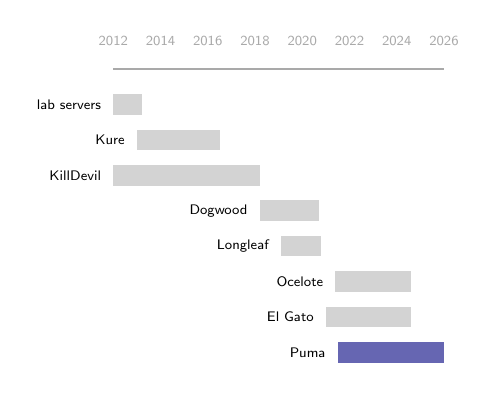
\begin{tikzpicture}[x=0.3cm, every node/.style={font=\tiny\sffamily}]
  \foreach \yr in {2012,2014,...,2026} \node[text=DarkGray] at (\yr-2012,0.35) {\yr};
  \draw[DarkGray] (0,0) -- (14,0);
  \foreach \n/\a/\b/\y in {lab servers/0/1.2/-0.45, Kure/1/4.5/-0.9, KillDevil/0/6.2/-1.35, Dogwood/6.2/8.7/-1.8, Longleaf/7.1/8.8/-2.25, Ocelote/9.4/12.6/-2.7, El Gato/9/12.6/-3.15}
    {\fill[LightGray] (\a,\y-0.13) rectangle (\b,\y+0.13); \node[anchor=east] at (\a-0.1,\y) {\n};}
  \fill[NavyBlue!60] (9.5,-3.6-0.13) rectangle (14,-3.6+0.13); \node[anchor=east] at (9.4,-3.6) {Puma};
\end{tikzpicture}}
\end{frame}

% 2
\begin{frame}{What this archive chapter is for}
\label{fr:why}
\begin{columns}[T,onlytextwidth]
\begin{column}{0.54\textwidth}
\footnotesize
\begin{itemize}\setlength{\itemsep}{3pt}
  \item \al{Reading old notes.} Twelve years of course notes, lab notes, job scripts and papers' methods sections refer to machines that no longer run: the lab's own Linux servers, UNC's Kure, KillDevil, Dogwood and Longleaf, and the University of Arizona's Ocelote and El Gato. This chapter keeps how they were used, so that an old note or script can be read and its run understood.
  \item \al{Legacy.} Every historical listing is marked ``historical, do not run'', and every slide carries the LEGACY label; a dash or curly quote that a shell would not accept is printed red. The host names, queues, modules and folders are gone; several commands carry slips that this chapter points out.
  \item \al{Most slides point to today's way}: chapters 1 (Puma, Slurm, storage), 2 (installing IBAMR), 3 (building and running) and 31 (VisIt on the cluster).
\end{itemize}
\end{column}
\begin{column}{0.43\textwidth}
\begin{punchbox}
\small Today the series runs on one cluster, Puma at the University of Arizona, with Slurm, IBAMR built by autoibamr, and a CMake build (chapters 1--3). Nothing in this chapter is needed to follow the rest of the series.
\end{punchbox}
\vspace{2mm}
\footnotesize Building the software on these machines is chapter X2; the code changes from one installed IBAMR to the next are chapter X3.
\end{column}
\end{columns}
\sourcecredit{The sources themselves, compared in October 2026.}
\end{frame}

% 3
\begin{frame}{Where these notes came from (1/2): 2012--2016}
\label{fr:sources1}
\tiny
\renewcommand{\arraystretch}{1.12}
\setlength{\tabcolsep}{3pt}
\begin{tabular}{@{}L{0.42\textwidth}L{0.08\textwidth}L{0.2\textwidth}L{0.25\textwidth}@{}}
\toprule
source & year & machines & author \\
\midrule
IBAMR ReadMe deck (lab) & 2012 & lab servers; KillDevil & the Miller lab (author not recorded) \\
``How to use the 3D IBAMR created by Boyce Griffith'' & 2012 & a lab server & Shannon Jones (``Tutorial by S. Jones'') \\
forces install deck & 2013 & lab servers; KillDevil & the Miller lab (author not verified) \\
``Install THLinux and IBAMR''; ``Running IBAMR on THLinux''; ``Running IBAMR on Killdevil'' & 2011--13 & the lab's servers; KillDevil & the instructor \\
MATH 564 homework 1 & 2013 & a lab server; KillDevil, Kure & the instructor \\
``IBAMR Killdevil Module'' (March 26, 2014) & 2014 & KillDevil & the instructor \\
``Using IBAMR Module on Kure - Instructions for Undergraduates'' & 2014 & Kure, KillDevil & not recorded \\
``The Joy of Immersed Boundary Methods with Adaptive Mesh Refinement'' (notes from the 2014 summer course) & 2014 & Kure & Dennis Evangelista (author line: ``People and Dennis Evangelista'') \\
``IBAMR Tutorial: UNC Edition'' (also MATH 769, Lecture 3, January 2015) & 2014--15 & Kure & not stated \\
``Party time in on super computers! (\ldots or how to run simulations on Kure/Kill Devil)'' & 2014 & Kure, KillDevil & Nick Battista \\
MATH 769, Lecture 1 (slide 11) & 2015 & Kure & the instructor \\
``Getting Running on IB2D and IBAMR'' (MATH 768) & 2016 & Kure, KillDevil & not stated \\
IB talk, 7 September 2016 & 2016 & Kure, KillDevil & Nick Battista and Laura A. Miller \\
\bottomrule
\end{tabular}
\sourcecredit{The sources themselves, compared in October 2026. Where a source does not state its author, it stays unattributed.}
\end{frame}

% 4
\begin{frame}{Where these notes came from (2/2): 2017--2024}
\label{fr:sources2}
\tiny
\renewcommand{\arraystretch}{1.12}
\setlength{\tabcolsep}{3pt}
\begin{tabular}{@{}L{0.42\textwidth}L{0.08\textwidth}L{0.2\textwidth}L{0.25\textwidth}@{}}
\toprule
source & year & machines & author \\
\midrule
``IBAMR Tutorial: Getting Started on UNC cluster'' & 2017--18 & KillDevil & not stated \\
TubeHeart ``Read me'' & 2017 & KillDevil & the instructor \\
``1 - Get killdevil account and software'' & 2018 & KillDevil & the instructor \\
``7-IBAMR- Running many simulations Part 2'' & 2018 & KillDevil & the instructor (two scripts by a student) \\
``Run your first IBAMR simulation'' & 2018 & KillDevil & Nick Battista (2014), adapted by the instructor \\
VisIt decks: ``Visit from command line and Python'', ``Analyzing your IBFE simulation'', ``Resampling AMR grids'' & 2017--18 & KillDevil & not stated; parts by Christopher Strickland and Lindsay Waldrop \\
IBFE ``Getting Started'' decks & 2014--18 & KillDevil & adapted from Alex Hoover's tutorial \\
``2-Run your IBAMR simulation on Dogwood''; ``Debugging Tips'' (2019) & 2018--20 & Dogwood & the instructor's course decks \\
Lecture 8: COMSOL workflow, export and run remotely & 2019--20 & Dogwood, Longleaf & the instructor \\
``Get dogwood account and run a simulation'' (Lecture 1) & 2020 & Dogwood & the instructor, adapted from Nick Battista (2014) \\
IBFE lecture 5 (``Plans for June''); Lecture 6 & 2020; 2025 & Dogwood; Puma & the instructor \\
VisIt on the cluster (Lecture 5 of the data course) & 2020 & Dogwood, Longleaf & G. Hobson \\
the course job scripts and Makefiles (\code{examples/legacy}) & 2014--24 & KillDevil, Dogwood, Ocelote, Puma & the course \\
UA cluster decks (``UAClusterIb2dIBAMR'', ``UA-HPC'') & 2021--22 & Puma, Ocelote, El Gato & the instructor \\
``Get HPC account and run a simulation'' (UA Lecture 1); Lecture 0 & 2024 & Puma, Ocelote, El Gato & the instructor (Lecture 1 adapted from Nick Battista, 2014) \\
\bottomrule
\end{tabular}
\sourcecredit{The sources themselves, compared in October 2026.}
\end{frame}

% 5
\begin{frame}{The machines, 2012--2026: a timeline}
\label{fr:timeline}
\begin{columns}[T,onlytextwidth]
\begin{column}{0.58\textwidth}
\centering
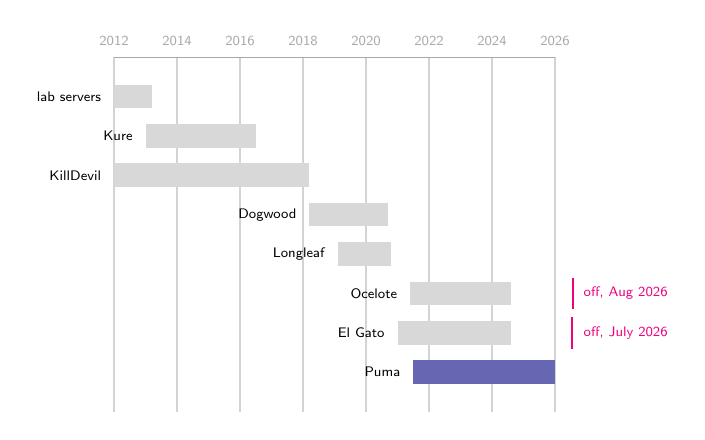
\begin{tikzpicture}[x=0.4cm, every node/.style={font=\tiny\sffamily}]
  \foreach \yr in {2012,2014,...,2026} {\node[text=DarkGray] at (\yr-2012,0.4) {\yr}; \draw[LightGray] (\yr-2012,0.2) -- (\yr-2012,-4.3);}
  \draw[DarkGray] (0,0.2) -- (14,0.2);
  \foreach \n/\a/\b/\y in {lab servers/0/1.2/-0.3, Kure/1/4.5/-0.8, KillDevil/0/6.2/-1.3, Dogwood/6.2/8.7/-1.8, Longleaf/7.1/8.8/-2.3, Ocelote/9.4/12.6/-2.8, El Gato/9/12.6/-3.3}
    {\fill[DarkGray!45] (\a,\y-0.15) rectangle (\b,\y+0.15); \node[anchor=east] at (\a-0.1,\y) {\n};}
  \fill[NavyBlue!60] (9.5,-3.8-0.15) rectangle (14,-3.8+0.15); \node[anchor=east] at (9.4,-3.8) {Puma};
  \draw[RubineRed,thick] (14.58,-2.8-0.2) -- (14.58,-2.8+0.2); \node[anchor=west,text=RubineRed] at (14.6,-2.8) {off, Aug 2026};
  \draw[RubineRed,thick] (14.55,-3.3-0.2) -- (14.55,-3.3+0.2); \node[anchor=west,text=RubineRed] at (14.6,-3.3) {off, July 2026};
\end{tikzpicture}
\end{column}
\begin{column}{0.39\textwidth}
\scriptsize
\begin{itemize}\setlength{\itemsep}{2pt}
  \item The bars mark the years in which the course's notes \al{used} each machine, not the machines' lifetimes. No source in the course's files states when Kure, KillDevil, Dogwood or Longleaf were retired.
  \item January 2018: ``the server used in most of the screenshots is kure. We now only use the server killdevil.''
  \item Ocelote moved to CentOS 7 and Slurm in June--July 2021 (an OnDemand banner: ``Ocelote downtime scheduled on 2021-06-01, 08:00 thru 2021-07-01, 08:00 for Upgrade to CentOS 7 and Slurm''; the deck of 11 July 2021: ``This cluster should be online July 12'').
  \item El Gato was shut down on 29 July 2026 and Ocelote on 17 August 2026 (chapter 1); Puma is the only UA cluster.
\end{itemize}
\end{column}
\end{columns}
\sourcecredit{The dates stated in the sources; chapter 1 for the 2026 shutdowns.}
\end{frame}

% 6
\begin{frame}[fragile]{Three ways a run was started, and today's}
\label{fr:threeways}
\begin{columns}[T,onlytextwidth]
\begin{column}{0.235\textwidth}
\scriptsize\al{Lab server, 2012}: no scheduler
\hist{2012 tutorial (fixed)}
\begin{lstlisting}[style=hist]
screen
mpirun -np 4 ./main3d input3d
# Ctrl+A Ctrl+D: detach
ps -u <user>
kill <pid>
\end{lstlisting}
\end{column}
\begin{column}{0.235\textwidth}
\scriptsize\al{LSF}: Kure, KillDevil, 2012--18
\hist{2014 notes}
\begin{lstlisting}[style=hist]
bsub -q week -n 8 mpirun ./main2d input2d
bjobs
bkill <jobid>
\end{lstlisting}
\end{column}
\begin{column}{0.235\textwidth}
\scriptsize\al{Slurm}: Dogwood 2018--20; Arizona 2021--24
\hist{after the 2020 notes; \code{<onyen>} for the user ID}
\begin{lstlisting}[style=hist]
sbatch script.sh
squeue -u <onyen>
scancel <jobid>
\end{lstlisting}
\end{column}
\begin{column}{0.235\textwidth}
\scriptsize\al{Today}: Puma (chapters 1 and 3)
\begin{lstlisting}[style=shell,basicstyle=\ttfamily\tiny\color{BlackGray}]
sbatch job.slurm
squeue --me
scancel <jobid>
\end{lstlisting}
\end{column}
\end{columns}
\vspace{2mm}
\small
\begin{itemize}\setlength{\itemsep}{2pt}
  \item On the lab's servers a run was started by hand and shared the machine with everyone else's; the users kept the peace by rules (slide \ref{fr:rules}).
  \item With LSF and Slurm a scheduler starts the run on compute nodes when the cores are free. On the UNC clusters the login node was for editing, building and submitting; on Puma it is for editing and submitting only, and builds run on a compute node too (chapters 1 and 3).
  \item Slurm's commands have barely changed since Dogwood; what changed is the job script around them (chapter 3).
\end{itemize}
\sourcecredit{Shannon Jones's 2012 tutorial (with the en dashes fixed); Nick Battista's 2014 notes; the 2020 Dogwood notes; chapter 3.}
\end{frame}

% 7
\begin{frame}{The lab's own Linux servers (2012)}
\label{fr:labservers}
\begin{columns}[T,onlytextwidth]
\begin{column}{0.55\textwidth}
\scriptsize
\begin{itemize}\setlength{\itemsep}{3pt}
  \item In 2012 the lab ran IBAMR on its own Ubuntu servers (Ubuntu 11.04 in the screenshots), shared by everyone in the lab. Their names are withheld here.
  \item The ReadMe deck began with ``Logging into a linux server'': download the SSH client that UNC's IT services offered, ``Open ssh, and click on Quick Connect'', and give the host name and your user name. Its slide also named a Unix tutorial on the web for newcomers.
  \item IBAMR was built in each user's home folder (\code{\$HOME/sfw}, chapter X2), and the examples ran from its build folder: \code{\$HOME/sfw/ibamr/\allowbreak ibamr-objs-opt/\allowbreak examples/...}.
  \item By September 2013 the two servers ran THLinux, UNC's ``Tar Heel Linux'', with one IBAMR built as root in \code{/usr/bin/sfw} for everyone (slide \ref{fr:screen2013}; chapter X2); when they changed from Ubuntu is not stated.
\end{itemize}
\end{column}
\begin{column}{0.42\textwidth}
\begin{homebox}
\footnotesize The first slide of the 2012 ReadMe also gave the server's login details. They are withheld here: login details never belong in shared notes or slides.
\end{homebox}
\vspace{2mm}
\footnotesize \al{Today}: you log in to Puma through the university's bastion host with your own NetID and two-step login (chapter 1).
\end{column}
\end{columns}
\sourcecredit{The Miller lab's IBAMR ReadMe deck (2012), slides 1--4; Shannon Jones's 2012 tutorial, slide 3 and screenshots; the instructor's ``Running IBAMR on THLinux'' (2013), slides 2 and 4--5; host names withheld.}
\end{frame}

% 8
\begin{frame}{Logging in and copying files with the 2012 SSH client}
\label{fr:sshclient}
\begin{columns}[T,onlytextwidth]
\begin{column}{0.5\textwidth}
\small
\begin{itemize}\setlength{\itemsep}{3pt}
  \item Two programs from UNC's IT services, ``SSH Secure Shell Client'' and ``SSH Secure File Transfer'' (an ONYEN, UNC's user ID, was needed to download them).
  \item \al{File transfer}: Quick Connect, then the host name and your user name, then the password; the window shows the local files on the left and the server's on the right, and files are dragged across. The 3D IBAMR files were ``under \code{sfw/ibamr/\allowbreak ibamr-objs-opt/\allowbreak examples/\allowbreak samples\_wings/}''.
  \item \al{Shell}: the same Quick Connect dialog opens a terminal on the server.
\end{itemize}
\end{column}
\begin{column}{0.47\textwidth}
\centering
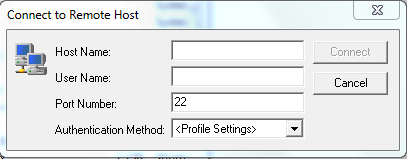
\includegraphics[width=\linewidth]{x1-ssh-connect-dialog-2012.png}

\vspace{1mm}
\scriptsize The client's ``Connect to Remote Host'' dialog (2012), empty.
\vspace{2mm}

\footnotesize \al{Today}: a terminal (Mac, Linux, Windows OpenSSH or WSL, or PuTTY) for the shell, and FileZilla or \code{scp} for files (chapter 1).
\end{column}
\end{columns}
\sourcecredit{Shannon Jones, ``How to use the 3D IBAMR created by Boyce Griffith'' (May 2012), slides 3--13; the screenshot from slide 6, cropped to the dialog.}
\end{frame}

% 9
\begin{frame}[fragile]{Finding your way on the server: \code{cd}, \code{ls}, Tab, \code{emacs}}
\label{fr:shell2012}
\begin{columns}[T,onlytextwidth]
\begin{column}{0.45\textwidth}
\hist{2012 tutorial, slides 14--21}
\begin{lstlisting}[style=hist]
cd sfw          # into a folder
cd ..           # one folder up
ls              # folders are shown in blue
# Tab completes a file or folder name
emacs update_target_point_positions.C   # edit a file; Ctrl+X Ctrl+C to leave
make clean
make main3d
\end{lstlisting}
\end{column}
\begin{column}{0.52\textwidth}
\small
\begin{itemize}\setlength{\itemsep}{3pt}
  \item The 2012 tutorial taught the shell from scratch, a command per slide.
  \item The files a user changed for a new run (slide 20): \code{input3d}, \code{update\_target\_point\_positions.C}, and the structure files \code{.vertex}, \code{.spring}, \code{.beam}, \code{.target}.
  \item After an edit: \code{make clean} and \code{make main3d}, then the run (slide \ref{fr:noscheduler}).
\end{itemize}
\vspace{1mm}
\footnotesize \al{Today}: the shell is chapter 1's subject (with nano and vi in place of emacs); the structure files are chapter 6's.
\end{column}
\end{columns}
\sourcecredit{Shannon Jones, ``How to use the 3D IBAMR created by Boyce Griffith'' (2012), slides 14--21 (the commands retyped; the comments are this chapter's).}
\end{frame}

% 10
\begin{frame}[fragile]{Building and rebuilding an example in your home folder (2012) (1/2)}
\label{fr:build2012}
\begin{columns}[T,onlytextwidth]
\begin{column}{0.48\textwidth}
\hist{ReadMe deck, slide 3, ``Running the code''}
\begin{lstlisting}[style=hist]
cd $HOME/sfw/ibamr/ibamr-objs-opt/examples/moving_plates2d
IBAMR_SRC_DIR   = /path/to/IBAMR
IBAMR_BUILD_DIR = /path/to/ibamr-objs-directory
% make clean
% make distclean
% make main2d
% ./main2d input2d
\end{lstlisting}
\hist{slides 7, 8 and 10 (the \code{\%} prompts left out; a slide's commands joined with \code{;})}
\begin{lstlisting}[style=hist]
# 3D: in .../examples/moving_plates3d
make clean
make cleandist
make main3d
./main3d input3d
# after editing update_target_point_positions.C:
rm -f main2d; make clean; make cleandist; make main2d
# other examples:
cd IB; cd staggered_grid; cd explicit; make examples; cd ex0; make main2d; ./main2d input2c
\end{lstlisting}
\end{column}
\begin{column}{0.49\textwidth}
\footnotesize
\begin{itemize}\setlength{\itemsep}{2pt}
  \item The \code{\%} is the deck's prompt; the two Makefile lines are the ones each example's Makefile had to point at the user's own IBAMR (chapter X3 dates code by them).
\end{itemize}
\vspace{1mm}
\al{Today}: CMake in a \code{build} folder, and runs on compute nodes (chapter 3).
\end{column}
\end{columns}
\sourcecredit{The Miller lab's IBAMR ReadMe deck (2012), slides 2--3 and 7--10.}
\end{frame}

% 10b
\begin{frame}{Building and rebuilding an example in your home folder (2/2): what the deck says}
\label{fr:build2012b}
\small
\begin{itemize}\setlength{\itemsep}{4pt}
  \item ``Simple clap and fling'' (\code{moving\_plates}): the left wing translates left and the right one right; a time step too large shows as ``an error quickly'' or ``very noisy'' results, and \code{dt} is set in the input file.
  \item The parameters (slide 9): \code{plate3d\_left\_512.\{vertex,\allowbreak spring,\allowbreak beam,\allowbreak target\}}, made by MATLAB scripts run twice, once per wing.
  \item \al{Slips}: \code{make cleandist} is a slip for \code{make distclean}, which the same deck writes on slides 3 and 7; \code{input2c} is \code{input2d}; the deck calls a generator ``generate\_meash3d.m'' (\code{generate\_mesh3d.m}).
\end{itemize}
\sourcecredit{The Miller lab's IBAMR ReadMe deck (2012), slides 2--3 and 7--10.}
\end{frame}

% 11
\begin{frame}[fragile]{Running without a scheduler: \code{screen}, \code{mpirun}, \code{ps}, \code{kill}}
\label{fr:noscheduler}
\begin{columns}[T,onlytextwidth]
\begin{column}{0.45\textwidth}
\hist{2012 tutorial, slide 27, ``Overview of IBAMR Commands'' (as written; two lines of its prose left out)}
\begin{lstlisting}[style=hist]
make clean
make main3d
screen (followed by enter)
mpirun –np 4 ./main3d input3d
<Ctrl+A><Ctrl+D> (to exit screen)
ps –u<user>
kill #####
\end{lstlisting}
\hist{ReadMe deck, slide 4, ``Doing a parallel run''}
\begin{lstlisting}[style=hist]
mpirun -np 4 ./main2d input2d
\end{lstlisting}
\end{column}
\begin{column}{0.52\textwidth}
\footnotesize
\begin{itemize}\setlength{\itemsep}{0.5pt}
  \item \code{screen} starts a terminal session that survives logging out; Ctrl+A then Ctrl+D detaches from it, and the run goes on; \code{screen -r} returns to it.
  \item \code{mpirun -np 4} starts four processes on the server itself; \code{ps -u <user>} lists your processes with their IDs, and \code{kill} stops one.
  \item \al{Slips}: the slides type en dashes (\code{\ndashmark{}np}, \code{\ndashmark{}u}, in red), which the programs (\code{mpirun}, \code{ps}) do not read as options; the speaker notes start the command with a capital M (\code{Mpirun}), and Linux commands are case-sensitive. (\code{ps -u<user>}, with no space, is fine: the tutorial's own screenshot shows it working.)
  \item The tutorial's \code{ps} screenshot shows \code{main3d} processes that had used up to four days of CPU time each on the shared server.
\end{itemize}
\vspace{0.5mm}
\al{Today}: never run on a login node; Slurm runs the job (chapter 3).
\end{column}
\end{columns}
\sourcecredit{Shannon Jones's 2012 tutorial, slides 22--27 and notes (the lab user name replaced by \code{<user>}); the Miller lab's ReadMe deck, slide 4.}
\end{frame}

% 11b
\begin{frame}[fragile]{The lab's servers in 2013 (1/2): \code{screen} and the library path}
\label{fr:screen2013}
\begin{columns}[T,onlytextwidth]
\begin{column}{0.53\textwidth}
\hist{``Running IBAMR on THLinux'' (2013), slide 4, as written}
\begin{lstlisting}[style=hist]
Go to the folder where you have your example code

(Advanced) On a new system, check the Makefile to make sure that
IBAMR_SRC_DIR   = /path/to/IBAMR
IBAMR_BUILD_DIR = /path/to/ibamr-objs-directory

For the two-dimensional case do
% screen
% export LD_LIBRARY_PATH=/usr/bin/sfw/linux/openmpi/1.4.3/lib
% make clean
% make main2d
% ./main2d input2d &
& Ctrl+A Ctrl+D (this exits the screen and it will run in the background.
\end{lstlisting}
\end{column}
\begin{column}{0.44\textwidth}
\footnotesize
\begin{itemize}\setlength{\itemsep}{2pt}
  \item By September 2013 the two servers ran THLinux with one IBAMR built as root in \code{/usr/bin/sfw} (chapter X2); the OpenMPI library path had to be typed in the terminal before each run (``every time you run main2d/3d''); adding it to \code{.bash\_profile} and \code{.bashrc} ``does not seem to fix it''.
  \item Ctrl+A then Ctrl+D \emph{detaches} from \code{screen} (it does not exit it): the run goes on, and \code{screen -r} returns to it later, which none of the old notes says. The \code{\&} before ``Ctrl+A'' is probably the \code{\%} prompt mistyped (the keys are pressed, not typed), and inside \code{screen} the \code{\&} after the command is not needed.
\end{itemize}
\vspace{1mm}
\al{Today}: a batch job on the compute nodes, not \code{screen} on a shared machine (chapter 3).
\end{column}
\end{columns}
\sourcecredit{The instructor's ``Running IBAMR on THLinux'' (created September 2013), slides 2, 4 and 6--7; ``Install THLinux and IBAMR'', slides 2, 5 and 21; ``Running IBAMR on Killdevil'' (2013), slide 5.}
\end{frame}

% 13b
\begin{frame}[fragile]{The lab's servers in 2013 (2/2): a tighter tolerance}
\label{fr:screen2013b}
\begin{columns}[T,onlytextwidth]
\begin{column}{0.53\textwidth}
\hist{slides 6--7, one line from each: ``Reducing error tolerance in fluid solver''; ``Reduced error tolerance and parallel submission command''}
\begin{lstlisting}[style=hist]
./main2d input2d -stokes_ksp_rtol 1.0e-9
mpirun -np 4 ./main2d input2d -stokes_ksp_rtol 1.0e-9
\end{lstlisting}
\end{column}
\begin{column}{0.44\textwidth}
\footnotesize
\begin{itemize}\setlength{\itemsep}{2pt}
  \item \code{-stokes\_ksp\_rtol 1.0e-9} tightens the Stokes solver's relative tolerance: ``Often this is needed for convergence''. It was also given after \code{mpirun} (slide 7) and, on KillDevil, after \code{bsub}: \code{bsub -q week -n 16 mpirun ./main2d input2d -stokes\_ksp\_rtol 1.0e-9} (``Running IBAMR on Killdevil'', slide 5).
\end{itemize}
\vspace{1mm}
\al{Today}: the same option works; the input file's solver block is the better place for it (chapter 16).
\end{column}
\end{columns}
\sourcecredit{The instructor's ``Running IBAMR on THLinux'' (created September 2013), slides 2, 4 and 6--7; ``Install THLinux and IBAMR'', slides 2, 5 and 21; ``Running IBAMR on Killdevil'' (2013), slide 5.}
\end{frame}


% 12
\begin{frame}{Sharing one server: the 2012 rules}
\label{fr:rules}
\begin{columns}[T,onlytextwidth]
\begin{column}{0.52\textwidth}
\small From the ReadMe deck, ``Doing a parallel run'':
\begin{itemize}\setlength{\itemsep}{3pt}
  \item one server ``has 24 processors, and'' the other ``16'';
  \item ``You want to use a power of 2'';
  \item ``Do not use all of the processors! Use no more than 16'' on the first ``and 8'' on the second;
  \item use fewer if others are running, and plan big runs together at lab meetings.
\end{itemize}
\end{column}
\begin{column}{0.45\textwidth}
\begin{punchbox}
\small These rules are what a scheduler enforces today. On Puma, Slurm gives each job the cores it asked for, holds the others until cores are free, and stops a job at its time limit (chapters 1 and 3).
\end{punchbox}
\vspace{2mm}
\footnotesize Slurm and IBAMR accept any number of processes; the series' job scripts ask for 4 (chapter 3).
\end{column}
\end{columns}
\sourcecredit{The Miller lab's IBAMR ReadMe deck (2012), slide 4 (server names withheld).}
\end{frame}

% 13
\begin{frame}[fragile]{Watching the time step in the log (2012)}
\label{fr:dtlog}
\begin{columns}[T,onlytextwidth]
\begin{column}{0.46\textwidth}
\hist{ReadMe deck, slide 5, ``Output (2D sims)''}
\begin{lstlisting}[style=hist]
% grep "dt = " IB2d.log
% tail -f IB2d.log | grep "dt = "
\end{lstlisting}
\small
\begin{itemize}\setlength{\itemsep}{3pt}
  \item The 2D examples wrote their visualization files to \code{viz\_IB2d} and their diagnostics to \code{IB2d.log}.
  \item \code{grep} prints the time-step lines; \code{tail -f} follows the log as the run writes it.
\end{itemize}
\end{column}
\begin{column}{0.51\textwidth}
\begin{homebox}
\footnotesize ``If you see that the timestep size decreases dramatically, this usually means that the computation has gone unstable. Reduce the value of `DT' in input2d and restart the model.''
\end{homebox}
\vspace{2mm}
\footnotesize The advice holds today. \code{IB2d.log} is the log file named in the input (\code{log\_file\_name}) of IBAMR's 2D examples, not a file of the IB2d software.

\vspace{1mm}
\al{Today}: the job's log and \code{.out} file (chapter 3); time steps and stability (chapter 16).
\end{column}
\end{columns}
\sourcecredit{The Miller lab's IBAMR ReadMe deck (2012), slides 2 and 5.}
\end{frame}

% 14
\begin{frame}{A 2013 homework on the lab server}
\label{fr:hw2013}
\begin{columns}[T,onlytextwidth]
\begin{column}{0.55\textwidth}
\small MATH 564, homework 1 (due 19 February 2013), told students where to run two of its examples (the bristles and the multiple boundaries):
\begin{itemize}\setlength{\itemsep}{3pt}
  \item they ``will need to be run on the new force installation of IBAMR, or on'' a lab server (the forces build of chapter X2);
  \item ``Please create a folder in'' the lab's shared folder ``if you wish to run simulations on'' that server;
  \item ``Copy these files to killdevil (kure) or your folder on'' the lab server.
\end{itemize}
\end{column}
\begin{column}{0.42\textwidth}
\footnotesize The homework itself (end times, plots at cycles 40000 and 100000, Reynolds-number questions) is in Appendix C, which maps it to today's examples.

\vspace{2mm}
In 2013 a course thus used three kinds of machine at once: the lab's servers, KillDevil, and Kure. The next part of this chapter is UNC's two clusters.
\end{column}
\end{columns}
\sourcecredit{The instructor's MATH 564 homework 1 (Spring 2013); server and folder names withheld.}
\end{frame}

% 15
\begin{frame}{Kure and KillDevil at a glance (2012--2018)}
\label{fr:kkglance}
\begin{columns}[T,onlytextwidth]
\begin{column}{0.55\textwidth}
\scriptsize
\begin{itemize}\setlength{\itemsep}{1.5pt}
  \item \al{Two UNC clusters} used from 2012 to 2018: Kure (``the machine where IBAMR jobs are run'', the 2014 notes say) and KillDevil. They shared the same software tree (\code{/nas02/apps}) and modules, so the same Makefile worked on both.
  \item \al{The scheduler was LSF}: \code{bsub} submits, \code{bjobs} lists, \code{bkill} stops (slides \ref{fr:bsub}--\ref{fr:bjobs}); the notes name the queues \code{week} (``longest queue''), \code{day}, \code{int}, \code{debug} and \code{ms} (copies to mass storage).
  \item \al{Software by modules}: \code{module list}, \code{module add}, \code{module initadd}; IBAMR itself from 2014 (\code{ibamr/3803}, then \code{ibamr/2016-11}).
  \item \al{Storage}: a home folder with a quota, the scratch space \code{/netscr/<onyen>}, emptied of files 21 days after they were last changed, and mass storage (\code{\textasciitilde/ms}); Kure and KillDevil shared all three.
  \item January 2018: ``the server used in most of the screenshots is kure. We now only use the server killdevil.''
\end{itemize}
\end{column}
\begin{column}{0.42\textwidth}
\centering
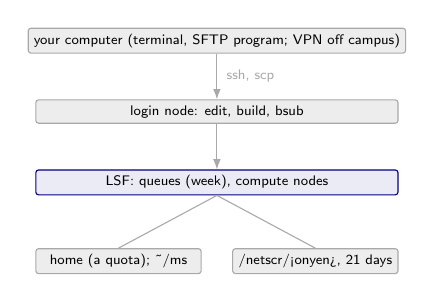
\begin{tikzpicture}[every node/.style={font=\tiny\sffamily}, box/.style={draw=DarkGray, fill=LightGray!40, rounded corners=1pt, align=center, inner sep=2pt}]
  \node[box, minimum width=4.6cm] (you) at (0,0) {your computer (terminal, SFTP program; VPN off campus)};
  \node[box, minimum width=4.6cm] (login) at (0,-0.9) {login node: edit, build, \code{bsub}};
  \node[box, minimum width=4.6cm, fill=NavyBlue!8, draw=NavyBlue] (lsf) at (0,-1.8) {LSF: queues (\code{week}), compute nodes};
  \node[box, minimum width=2.1cm] (home) at (-1.25,-2.8) {home (a quota); \code{\textasciitilde/ms}};
  \node[box, minimum width=2.1cm] (scr) at (1.25,-2.8) {\code{/netscr/<onyen>}, 21 days};
  \draw[-{Latex[length=1.3mm]},DarkGray] (you) -- node[right]{\code{ssh}, \code{scp}} (login);
  \draw[-{Latex[length=1.3mm]},DarkGray] (login) -- (lsf);
  \draw[DarkGray] (lsf.south) -- (home.north); \draw[DarkGray] (lsf.south) -- (scr.north);
\end{tikzpicture}
\end{column}
\end{columns}
\sourcecredit{The 2014 notes (Dennis Evangelista; ``IBAMR Tutorial: UNC Edition''; Nick Battista); ``Getting Running on IB2D and IBAMR'' (2016), slide 9; ``Run your first IBAMR simulation'' (2018); ``Using IBAMR Module on Kure'' (May 2014). Retirement dates are not stated in the course's files.}
\end{frame}

% 16
\begin{frame}{Getting an account: Onyen Services}
\label{fr:onyen}
\footnotesize
\begin{itemize}\setlength{\itemsep}{2pt}
  \item Every UNC person had an ONYEN (``Only Name You'll Ever Need''), the user ID for every campus service.
  \item A cluster account was one more service: on the ONYEN web page, ``Select subscribe to services, and then select Kure'' (2014; later KillDevil, then Dogwood).
  \item The 2014 summer-course notes put it the same way: Kure access through ONYEN Services, after which Kure is ``the machine where IBAMR jobs are run''.
  \item January 2018: ``Subscribe to Services'', then ``KillDevil Cluster''. The page could answer ``You are ineligible for the following services for the reasons cited: KillDevil Cluster: missing \code{'(LIVE|EXCH)'} prerequsite.'' [\emph{sic}]; an e-mail to Research Computing then did it (slide \ref{fr:dwaccount}, where the 2020 Dogwood guide keeps this text).
\end{itemize}
\vspace{2mm}
\begin{punchbox}
\footnotesize \al{Today}: a University of Arizona HPC account comes from the HPC portal; a faculty member (your PI) sponsors you and adds you to their group, whose allocation your jobs use (chapter 1).
\end{punchbox}
\sourcecredit{``IBAMR Tutorial: UNC Edition'' (May 2014), slide 2; Dennis Evangelista's notes (2014), section 2; ``1 - Get killdevil account and software'' (January 2018), step 1; ``Get dogwood account and run a simulation'' (2020), step 1.}
\end{frame}

% 17
\begin{frame}{From your computer: a terminal, an SFTP program, and VPN}
\label{fr:fromcomputer}
\begin{columns}[T,onlytextwidth]
\begin{column}{0.53\textwidth}
\scriptsize
\begin{itemize}\setlength{\itemsep}{2pt}
  \item \al{A terminal}: on a Mac, the Terminal (found with Spotlight); on Windows, PuTTY or the SSH program from UNC's software site; on Linux, OpenSSH (\code{ssh}, \code{sftp}), installed with \code{apt-get}.
  \item \al{An SFTP program} to move files: FileZilla (``Install filezilla or another sftp program to move files on and off kure'', the 2015 first-week checklist).
  \item \al{VPN} off campus: ``you will also need to use VPN (very private network)'' [\emph{virtual} private network]; on Ubuntu, \code{vpnc} and \code{network-manager-vpnc}.
  \item A plain-text editor that ``won't add random hidden characters (like Word)'': Notepad++ or Sublime (2018). In FileZilla or Fetch: host \code{kure.unc.edu}, port 22, remote folder \code{/netscr/onyen} (2014).
  \item The 2015 first-week checklist also asked for two screenshots, posted to the course site: ``a terminal opened that is logged into kure'' and VisIt.
\end{itemize}
\end{column}
\begin{column}{0.44\textwidth}
\footnotesize \al{The 2014 terminal basics} (Nick Battista's notes):

\vspace{1mm}
\scriptsize
\renewcommand{\arraystretch}{1.05}
\setlength{\tabcolsep}{3pt}
\begin{tabular}{@{}L{0.42\linewidth}L{0.55\linewidth}@{}}
\toprule
\code{pwd} & where am I \\
\code{cd ..}, \code{cd [folder\_name]} & up one folder; into a folder \\
\code{ls}, \code{ls -a} & list (with hidden files) \\
\code{mkdir [name]} & make a folder \\
\code{rm [name]}, \code{rm -r [folder\_name]} & remove a file; a folder \\
\code{cp [file1] [file2]} & copy a file \\
\code{cp -r [folder\_name1] [folder\_name2]} & copy a folder \\
\bottomrule
\end{tabular}

\vspace{1mm}
\footnotesize \al{Today}: chapter 1 (terminals, FileZilla, no VPN for SSH).
\end{column}
\end{columns}
\sourcecredit{``IBAMR Tutorial: UNC Edition'' (2014), slide 2; Dennis Evangelista's notes (2014); Nick Battista, ``Party time in on super computers!'' (August 2014), pages 1--2; MATH 769 Lecture 1 (January 2015), slide 11; ``Using IBAMR Module on Kure'' (May 2014); ``1 - Get killdevil account and software'' (January 2018), steps 2--6.}
\end{frame}

% 18
\begin{frame}[fragile]{Logging in, and the rule about the login node}
\label{fr:kklogin}
\begin{columns}[T,onlytextwidth]
\begin{column}{0.48\textwidth}
\hist{2014 notes; the second line from the 2017--18 KillDevil deck, slide 2 (placeholders for the ONYEN)}
\begin{lstlisting}[style=hist]
ssh <onyen>@kure.unc.edu
ssh <onyen>@killdevil.unc.edu
# the ONYEN password, then:
cd /netscr/<onyen>/
\end{lstlisting}
\begin{homebox}
\footnotesize ``repeat after me -- WE DO NOT RUN SIMULATIONS ON THE LOGIN NODE''
\end{homebox}
\end{column}
\begin{column}{0.49\textwidth}
\scriptsize
\begin{itemize}\setlength{\itemsep}{2pt}
  \item The login node is the machine \code{ssh} lands on, shared by everyone logged in. It was for editing, building and submitting; runs went to the compute nodes through the scheduler.
  \item The prompt showed the login node: \code{kure-login1}, \code{killdevil-login1}, \code{killdevil-login2}. The 2014 Kure deck itself shows a \code{killdevil-login1} prompt in its listings (slides 3 and 5).
  \item Dennis Evangelista's notes write \code{ssh kure.unc.edu} without the ONYEN, which works only when the user name on your own computer is the ONYEN (or an SSH configuration file supplies it).
\end{itemize}
\vspace{1mm}
\al{Today}: \code{ssh <netid>@hpc.arizona.edu}, then \code{shell}; a stricter rule: neither runs nor builds on the login node (chapter 1).
\end{column}
\end{columns}
\sourcecredit{Nick Battista, ``Party time in on super computers!'' (2014), pages 2--3 (Part I, steps 7--9); ``IBAMR Tutorial: UNC Edition'' (2014), slides 2--5; Dennis Evangelista's notes (2014), section 3.1.}
\end{frame}

% 19
\begin{frame}{Home, \code{/netscr} and keeping data}
\label{fr:netscr}
\begin{columns}[T,onlytextwidth]
\begin{column}{0.53\textwidth}
\scriptsize
\begin{itemize}\setlength{\itemsep}{3pt}
  \item ``It is important to remember NOT to run simulations in your home directory!! All simulations need to be run in the scratch file directory /netscr/onyen/'' (2014).
  \item ``the files in scratch file directory will be deleted in 21 days after the modification of the file''; ``files in the netscr directories are deleted 21 days after they are last modified''.
  \item ``Note that your home directory only has $\sim$ 5 GB. Also, all files are deleted every few weeks from netscr, so do not store data there long term!'' (2016).
  \item The home quota differed by account and year: ``My quota is 10,240 Megabytes, and the hard limit is 15360 Megabytes'' (one account, 2014); \code{quota} showed the use and both limits, \code{du -hs} a folder's size; ``if you exceed your quota, your simulation can be terminated.''
  \item Results were copied off ``at least within a week'' (slide \ref{fr:results}), or to mass storage (next slide).
\end{itemize}
\end{column}
\begin{column}{0.44\textwidth}
\begin{punchbox}
\small \al{Today on Puma}: \code{/home} (50 GB), \code{/xdisk/<pi>/<netid>} for runs (150 days, extendable once by 150), \code{/groups/<pi>} (500 GB) for what the group keeps (chapter 1). The rule is the same: run in the scratch space, keep results elsewhere.
\end{punchbox}
\end{column}
\end{columns}
\sourcecredit{``IBAMR Tutorial: UNC Edition'' (2014), slides 3 and 6; Dennis Evangelista's notes (2014), section 3.2; ``Getting Running on IB2D and IBAMR'' (2016), slide 9; Nick Battista's notes (2014); ``Using IBAMR Module on Kure'' (May 2014), ``General commands''.}
\end{frame}

% 19b
\begin{frame}[fragile]{Mass storage on Kure and KillDevil}
\label{fr:ms}
\begin{columns}[T,onlytextwidth]
\begin{column}{0.5\textwidth}
\hist{``Using IBAMR Module on Kure'' (May 2014)}
\begin{lstlisting}[style=hist]
cd ~/ms
bsub -q ms cp /netscr/onyen/text.txt /ms/home/o/n/onyen
\end{lstlisting}
\hist{``Running many simulations Part 2'' (March 2018), slide 15}
\begin{lstlisting}[style=hist]
bsub -q ms cp /netscr/myonyen/output/* /ms/home/m/y/myonyen/saved_output
\end{lstlisting}
\scriptsize \code{onyen} and \code{myonyen} are the sources' own placeholders; \code{o/n} and \code{m/y} are the first two letters of the user ID.
\end{column}
\begin{column}{0.47\textwidth}
\footnotesize
\begin{itemize}\setlength{\itemsep}{2pt}
  \item The \code{ms} folder in each home was the door to UNC's mass storage, a tape archive for finished or very large files: not a place to work, and not a backup.
  \item Jobs running under LSF could not read it; data had to be copied back to \code{/netscr} first.
  \item Many small files went in as one \code{tar} or \code{zip} file.
  \item Large copies went through LSF's \code{ms} queue, on hosts with fast access to the archive, not on the login node.
\end{itemize}
\vspace{1mm}
\al{Today}: \code{/groups/<pi>} for what the group keeps, and your own copies off the cluster (chapter 1).
\end{column}
\end{columns}
\sourcecredit{``Using IBAMR Module on Kure - Instructions for Undergraduates'' (May 2014; author not recorded), section ``Mass Storage'' (paraphrasing UNC's help page); ``7-IBAMR- Running many simulations Part 2'' (March 2018), slide 15.}
\end{frame}


% 20
\begin{frame}[fragile]{What the \code{module} command did}
\label{fr:modulecmd}
\begin{columns}[T,onlytextwidth]
\begin{column}{0.5\textwidth}
\hist{``IBAMR Tutorial: UNC Edition'' (2014), slides 4--5; the module list as printed in Dennis Evangelista's notes}
\begin{lstlisting}[style=hist]
module list
  1) null
module initadd ibamr/3803
exit
# log in again
module list
Currently Loaded Modulefiles:
  1) null                 4) petsc/3.4            7) boost/1.53.0
  2) openmpi_intel/11.1   5) libmesh/0.9.3        8) ibamr/3803
  3) hdf5/1.8.5           6) silo/4.9.1
\end{lstlisting}
\vspace{1mm}
\scriptsize \code{module rm} removed one, \code{module initrm} removed it from the start-up files, and \code{module initlist} listed what later logins would load. The 2014 Kure guide lists ``the basic module commands'', \code{module [ add | avail | help | list | load | initadd | unload | initrm | show ]} (its glossary adds \code{rm} and \code{initlist}), and the rule: initadd ``does not change your current session, only later logins.''
\end{column}
\begin{column}{0.47\textwidth}
\scriptsize
\begin{itemize}\setlength{\itemsep}{1pt}
  \item ``Check that you only have the null module'': a fresh account loaded nothing (\code{null}).
  \item \code{module add} loads a module for the current session; \code{module initadd} writes it into the shell's start-up files, so that it loads \al{at every login}. That is why the notes say to log out and back in.
  \item \code{module initadd ibamr/3803} brought the six modules IBAMR needed with it (the second listing, as printed in Dennis Evangelista's notes: seven entries after \code{null}, \code{ibamr/3803} included).
\end{itemize}
\al{Today}: \code{module load gnu13 openmpi5} inside each job script; IBAMR is your own autoibamr install, loaded with \code{enable.sh} (chapters 1--3).
\end{column}
\end{columns}
\sourcecredit{``IBAMR Tutorial: UNC Edition'' (2014), slides 4--5; Dennis Evangelista's notes (2014), section 3.1; ``Using IBAMR Module on Kure'' (May 2014); the 2016--17 module notes (chapter X2).}
\end{frame}

% 21
\begin{frame}[fragile]{The \code{ibamr/3803} module (2014--2016), and its runtime error}
\label{fr:m3803}
\begin{columns}[T,onlytextwidth]
\begin{column}{0.52\textwidth}
\footnotesize
\begin{itemize}\setlength{\itemsep}{2pt}
  \item IBAMR revision 3803 with the libraries of the last slide: ``Feb. 2014 (?)'' in the course Makefiles, and a deck dated ``March 26, 2014'' loads it (``You must first remove any other module'': \code{module remove openmpi\_\_\_}, then \code{module add ibamr/3803}); used by the course until late 2016.
  \item With it, a job could stop at once with a missing Intel library; the 2014 notes give the error and the fix, typed before \code{bsub}:
\end{itemize}
\hist{``IBAMR Tutorial: UNC Edition'' (2014), slide 11}
\begin{lstlisting}[style=hist]
/usr/mpi/intel/openmpi-1.4.1/bin/orted: error while loading shared libraries: libimf.so: cannot open shared object file: No such file or directory
export LD_LIBRARY_PATH=/nas02/apps/intel-11.1/cc/lib/intel64/
\end{lstlisting}
\end{column}
\begin{column}{0.45\textwidth}
\footnotesize
\begin{itemize}\setlength{\itemsep}{2pt}
  \item The module's OpenMPI was built with Intel's compilers; its daemon \code{orted} needs Intel's run-time library \code{libimf.so}; the \code{export} sets the library path to Intel's folder alone (ending it with \code{:\$LD\_LIBRARY\_PATH} would have kept the rest). \al{Today}: no \code{LD\_LIBRARY\_PATH} line; \code{enable.sh} sets the paths (chapter 2).
  \item Dennis Evangelista's notes put the \code{export} between \code{make main2d} and \code{bsub}, and warn that with wrong library paths a job ``will halt in about a minute''.
  \item The build side of this module (what it contained, how to build a newer IBAMR against it) is in chapter X2.
\end{itemize}
\end{column}
\end{columns}
\sourcecredit{``IBAMR Tutorial: UNC Edition'' (2014), slide 11; Dennis Evangelista's notes (2014), section 3.3; the course Makefiles' comments; ``IBAMR Killdevil Module'' (March 26, 2014), slides 1--4 and 9.}
\end{frame}

% 22
\begin{frame}[fragile]{The \code{ibamr/2016-11} module (2016--2018)}
\label{fr:m201611}
\begin{columns}[T,onlytextwidth]
\begin{column}{0.5\textwidth}
\hist{``Getting Started on UNC cluster'' (2017--18), slides 4--5}
\begin{lstlisting}[style=hist]
module initadd ibamr/2016-11
[<onyen>@killdevil-login2 ~]$ module list
  1) git/1.8.5.3         2) openmpi_gcc/4.8.1   3) python/2.6.5        4) ibamr/2016-11
\end{lstlisting}
\hist{``Run your first IBAMR simulation'' (January 2018; the module list retyped from its screenshot)}
\begin{lstlisting}[style=hist]
module initadd ibamr/2016-11
module list
  1) openmpi_gcc/4.8.1   2) python/2.6.5   3) ibamr/2016-11
\end{lstlisting}
\end{column}
\begin{column}{0.47\textwidth}
\footnotesize
\begin{itemize}\setlength{\itemsep}{2pt}
  \item The second IBAMR module (``Nov 2016'' in the course Makefiles), built on the \code{openmpi\_gcc/4.8.1} module (Open MPI with the GNU 4.8.1 compilers); the course used it on KillDevil (``We now only use the server killdevil'', 2018).
  \item The 2018 handout added a link to UNC's ``getting started on KillDevil'' help page, and a note that most of its screenshots still showed Kure.
  \item Moving between \code{ibamr/3803}, \code{ibamr/2016-11} and a home build needed \code{module initrm} of the others first (chapter X2); the course's IB examples were moved to this module early in 2017 (chapter X3).
\end{itemize}
\end{column}
\end{columns}
\sourcecredit{``IBAMR Tutorial: Getting Started on UNC cluster'' (2017--18), slides 4--5 (prompt scrubbed); ``Run your first IBAMR simulation'' (2018), adapted from Nick Battista's 2014 notes.}
\end{frame}

% 23
\begin{frame}[fragile]{KillDevil before the IBAMR module (2012--2013)}
\label{fr:kdearly}
\begin{columns}[T,onlytextwidth]
\begin{column}{0.53\textwidth}
\hist{ReadMe deck, slide 16 (2012)}
\begin{lstlisting}[style=hist]
export FC=gfortran CC=gcc CXX=g++ F77=gfortran
module add openmpi_gcc; module initadd openmpi_gcc
\end{lstlisting}
\hist{forces deck, slide 2 (2013)}
\begin{lstlisting}[style=hist]
export FC=gfortran CC=gcc CXX=g++ F77=gfortran
module initadd openmpi_gcc/4.4.6
\end{lstlisting}
\hist{ReadMe deck, slide 31; forces deck, slide 14 (two lines of prose left out)}
\begin{lstlisting}[style=hist]
Put the folder with your specific code into the /netscr/onyen folder. Then cd into the folder.
make clean
make main3d
bsub -q week -n 16 mpirun ./main3d input3d
*-n 16 will run on 16 processors. I recommend running 16-32 (should be powers of 2).
Type bjobs -uonyen to check on the status.
\end{lstlisting}
\end{column}
\begin{column}{0.44\textwidth}
\footnotesize
\begin{itemize}\setlength{\itemsep}{2pt}
  \item Before 2014 each user built IBAMR in the home folder (chapter X2) with KillDevil's GNU compilers and its \code{openmpi\_gcc} module; the \code{export} line chose the GNU compilers.
  \item The run was already the LSF pattern of the next six years: copy the folder to \code{/netscr}, \code{make clean}, \code{make main3d}, \code{bsub}.
  \item \code{bjobs -uonyen}: \code{-u} with the user ID written right after it; ``onyen'' stands for your own.
\end{itemize}
\end{column}
\end{columns}
\sourcecredit{The Miller lab's IBAMR ReadMe deck (2012), slides 16 and 31; the forces install deck (2013), slides 2 and 14.}
\end{frame}

% 23b
\begin{frame}[fragile]{Your own build on KillDevil (2013): the Makefile, and the \code{\$HOME} trap}
\label{fr:a4make}
\begin{columns}[T,onlytextwidth]
\begin{column}{0.53\textwidth}
\hist{``Running IBAMR on Killdevil'' (2013), slide 2, as written (the home path as \code{<o>/<n>/<user>})}
\begin{lstlisting}[style=hist]
In the make file, change the paths to the following:
IBAMR_SRC_DIR = $HOME/sfw2/ibamr/IBAMR2
IBAMR_BUILD_DIR = $HOME/sfw2/ibamr/ibamr-objs-opt

In a lot of the example codes, one one set of paths might be commented out so that you can switch back and forth between killdevil and a THLinux box.

Warning - Something changed on killdevil so my home directory was messed up, and I had to put in the full path.
IBAMR_SRC_DIR = /nas02/home/<o>/<n>/<user>/sfw2/ibamr/IBAMR2
IBAMR_BUILD_DIR = /nas02/home/<o>/<n>/<user>/sfw2/ibamr/ibamr-objs-opt
\end{lstlisting}
\end{column}
\begin{column}{0.44\textwidth}
\begin{homebox}
\footnotesize \al{The likely cause.} In a Makefile, \code{\$HOME} is not the shell's variable: \code{make} reads \code{\$H} (a one-letter variable, empty) followed by \code{OME}, so the path becomes \code{OME/sfw2/...} (checked with GNU Make 4.3). Make needs \code{\$(HOME)}, which the 2016-11 Makefiles write (in a commented-out line); the full path worked for the same reason.
\end{homebox}
\vspace{1mm}
\scriptsize ``one one [\emph{sic}] set of paths might be commented out'': the habit that left every era's paths as comments in the course Makefiles (chapter X3). The build itself, in \code{\$HOME/sfw2}, is chapter X2's.

\vspace{1mm}
\al{Today}: a \code{CMakeLists.txt}; no paths to write (chapter 3).
\end{column}
\end{columns}
\sourcecredit{The instructor's ``Running IBAMR on Killdevil'' (created September 2013), slide 2 (the home path shown with placeholders).}
\end{frame}


% 24
\begin{frame}[fragile]{Pointing a Makefile at the module}
\label{fr:makemodule}
\begin{columns}[T,onlytextwidth]
\begin{column}{0.56\textwidth}
\hist{IBFE ``Getting Started'' decks, slides 6--7}
\begin{lstlisting}[style=hist]
Makefile flags (for ibamr/3803)
LIBSNEW = $(LIBS) -lnetcdf -lcurl
IBAMR_SRC_DIR = /nas02/apps/ibamr-3803/OFED-1.5.2/IBAMR2
IBAMR_BUILD_DIR = /nas02/apps/ibamr-3803/ibamr-objs-opt

Makefile flags (for ibamr/2016-11)
LIBSNEW = $(LIBS) -lnetcdf -lcurl
IBAMR_SRC_DIR = /nas02/apps/ibamr-2016-11/OFED-1.5.2/sfw/ibamr/IBAMR
IBAMR_BUILD_DIR = /nas02/apps/ibamr-2016-11/OFED-1.5.2/sfw/ibamr/ibamr-objs-opt
\end{lstlisting}
\end{column}
\begin{column}{0.41\textwidth}
\footnotesize
\begin{itemize}\setlength{\itemsep}{2pt}
  \item Each example's Makefile named the module's source and build folders; IBFE examples also used \code{\$(LIBSNEW)} ``instead of the \$(LIBS) flag'' on their link lines.
  \item The course's later Makefiles often keep earlier installs' paths as comments (the 2016-11 ones list four install locations, three of them commented out), up to Dogwood's and Arizona's: chapter X3 dates old code by them; chapter X2 tells the story of the installs whose recipes survive.
\end{itemize}
\vspace{1mm}
\al{Today}: a \code{CMakeLists.txt} with \code{find\_package(IBAMR)}; an old Makefile stops at its \code{make.inc} line (chapter 3).
\end{column}
\end{columns}
\sourcecredit{The IBFE ``Getting Started'' decks (adapted from Alex Hoover's 2014 tutorial; updated 2017--18), slides 6--7.}
\end{frame}

% 25
\begin{frame}[fragile]{Copying an example up: \code{scp}, FileZilla, \code{zip}}
\label{fr:scp}
\begin{columns}[T,onlytextwidth]
\begin{column}{0.53\textwidth}
\hist{Nick Battista's notes (2014), as written}
\begin{lstlisting}[style=hist]
scp –r 1st_Simulation [your onyen]@kure.unc.edu:/netscr/[your onyen]
\end{lstlisting}
\hist{Dennis Evangelista's notes (2014)}
\begin{lstlisting}[style=hist]
desktop$ scp FlowTank.zip <onyen>@kure.unc.edu:/netscr/<onyen>/FlowTank.zip
desktop$ ssh kure.unc.edu
<onyen>@kure-login$ cd /netscr/<onyen>/
<onyen>@kure-login$ unzip FlowTank.zip
<onyen>@kure-login$ cd FlowTank
\end{lstlisting}
\end{column}
\begin{column}{0.44\textwidth}
\footnotesize
\begin{itemize}\setlength{\itemsep}{2pt}
  \item From the folder on your own computer that holds the example, \code{scp -r} copies a whole folder; ``the colon, : , is necessary'' between the host and the remote path.
  \item \al{A slip}: the notes' text has an en dash (\code{\ndashmark{}r}, in red); the screenshot beside it shows the hyphen that works.
  \item Or zip the example, copy one file, and \code{unzip} it on the cluster; or drag it across in FileZilla to ``your netscr/onyen directory on kure''.
\end{itemize}
\vspace{1mm}
\al{Today}: \code{scp}, \code{rsync} or FileZilla to \code{filexfer.hpc.arizona.edu} (chapter 1).
\end{column}
\end{columns}
\sourcecredit{Nick Battista's notes (2014), pages 4--5; Dennis Evangelista's notes (2014), section 3.2 (prompts with placeholders); ``IBAMR Tutorial: UNC Edition'' (2014), slide 8.}
\end{frame}

% 26
\begin{frame}[fragile]{Building on the login node: \code{make clean}, \code{make main2d}}
\label{fr:loginbuild}
\begin{columns}[T,onlytextwidth]
\begin{column}{0.47\textwidth}
\hist{Nick Battista's notes (2014), retyped; \code{make clean} from the 2014 Kure deck, slide 9}
\begin{lstlisting}[style=hist]
cd /netscr/<onyen>/1st_Simulation
make clean
make main2d
ls
\end{lstlisting}
\footnotesize ``New files'' after \code{make main2d}: \code{main2d}, \code{main.o}, \code{stamp-2d}, \code{update\_target\_point\_positions.o}. The example folder also held \code{hier\_data\_IB2d}, \code{IB2d.log} and \code{viz\_IB2d} after a run, the MATLAB scripts that made its geometry, and its \code{.target} and \code{.vertex} files.
\end{column}
\begin{column}{0.5\textwidth}
\footnotesize
\begin{itemize}\setlength{\itemsep}{2pt}
  \item Building ran on the login node, as every course handout from 2012 to 2024 did: a few minutes of one core, tolerated where runs were not.
  \item \code{make clean} removed old object files first, so that a new module or a changed header was compiled from scratch (\code{make} recompiles a changed \code{.C} file by itself).
  \item \code{stamp-2d} is the Makefile's marker of the last dimension built (chapter X3).
\end{itemize}
\vspace{1mm}
\al{Today}: \code{cmake} in an \code{interactive} session or a short batch job; the build folder is \code{build} (chapter 3).
\end{column}
\end{columns}
\sourcecredit{Nick Battista's notes (2014), pages 5 and 7 (Part I, steps 15--18 and 21) (the listing retyped from the screenshots, with the ONYEN replaced); ``IBAMR Tutorial: UNC Edition'' (2014), slide 9.}
\end{frame}

% 27
\begin{frame}[fragile]{Submitting with LSF: \code{bsub}}
\label{fr:bsub}
\begin{columns}[T,onlytextwidth]
\begin{column}{0.47\textwidth}
\hist{2014 Kure deck, slide 9}
\begin{lstlisting}[style=hist]
make clean
make main2d
bsub -q week -n 2 mpirun ./main2d input2d
\end{lstlisting}
\hist{Nick Battista's notes (2014)}
\begin{lstlisting}[style=hist]
bsub -q week -n 8 mpirun ./main2d input2d
Job <885471> is submitted to queue <week>.
\end{lstlisting}
\hist{IB talk (2016), page 74}
\begin{lstlisting}[style=hist]
module load ibamr/3803
make clean
make main2d
bsub -q week -n 4 mpirun ./main2d input2d
\end{lstlisting}
\end{column}
\begin{column}{0.5\textwidth}
\footnotesize ``bsub is the command to submit a simulation to the cluster. -q is a flag requesting a week queue (longest queue). -n is the number of processors. mpirun: multiple processors.''
\begin{itemize}\setlength{\itemsep}{2pt}
  \item \code{bsub} (``batch submit'') took the command line itself; the notes used no job script. LSF printed the job's number, which the 2014 notes ask you to record with what the run was (the Reynolds number, the time step, the output interval).
  \item The counts in the notes: 2, 4 and 8 for 2D, 16 to 32 for 3D, ``should be powers of 2''.
  \item LSF e-mailed when a job finished or ``halted abnormally''.
\end{itemize}
\vspace{1mm}
\al{Today}: a job script with \code{\#SBATCH} lines and \code{mpirun -np "\$SLURM\_NTASKS"}, submitted with \code{sbatch} (chapter 3).
\end{column}
\end{columns}
\sourcecredit{``IBAMR Tutorial: UNC Edition'' (2014), slide 9; Nick Battista's notes (2014), pages 5--6 (Part I, step 19); Dennis Evangelista's notes (2014), section 3.3; IB talk by Nick Battista and Laura A. Miller (7 September 2016), page 74.}
\end{frame}

% 28
\begin{frame}[fragile]{Watching and stopping LSF jobs: \code{bjobs}, \code{bkill}}
\label{fr:bjobs}
\begin{columns}[T,onlytextwidth]
\begin{column}{0.58\textwidth}
\hist{Nick Battista's notes (2014), the screenshot retyped}
\begin{lstlisting}[style=hist]
[<onyen>@kure-login1 1st_Simulation]$ bsub -q week -n 8 mpirun ./main2d input2d
Job <885471> is submitted to queue <week>.
[<onyen>@kure-login1 1st_Simulation]$ bjobs
JOBID   USER    STAT  QUEUE   FROM_HOST    EXEC_HOST    JOB_NAME    SUBMIT_TIME
885471  <onyen> RUN   week    kure-login1  8*public_ho  *d input2d  Aug 26 14:32
\end{lstlisting}
\hist{``Using IBAMR Module on Kure'' (May 2014)}
\begin{lstlisting}[style=hist]
bsub - submit
bqueues - tells you about traffic on the queues
Can use debug queue to test if things work, int or day for interactive
bkill - kills a job
bjobs - tells you information about your current jobs. Use this to check on the status of your submitted jobs.
bjobs -l gives more information
bhist - tells you information about your job history
bpeek lets you see the output that is happening
Killdevil/Kure will send you an email when your simulation finishes running (or fails to run).
\end{lstlisting}
\end{column}
\begin{column}{0.39\textwidth}
\footnotesize
\begin{itemize}\setlength{\itemsep}{2pt}
  \item \code{bjobs} works from any folder; it shows each job's state (\code{RUN} or \code{PEND}ing), its number, its processors and when it was submitted.
  \item \code{bjobs -u<onyen>} for one user; \code{bkill <jobid>} stops a job, \code{bkill 0} all of yours.
\end{itemize}
\vspace{1mm}
\al{Today}: \code{squeue --me}, \code{scancel <jobid>}, \code{sacct} for finished jobs (chapter 1).
\end{column}
\end{columns}
\sourcecredit{Nick Battista's notes (2014), page 6 (Part I, step 20) (the screenshot retyped, the user name replaced); ``IBAMR Tutorial: UNC Edition'' (2014), slide 10; Dennis Evangelista's notes (2014), section 3.3; ``Using IBAMR Module on Kure'' (May 2014).}
\end{frame}

% 29
\begin{frame}{Following the log on the cluster (1/2): \code{nano}}
\label{fr:nano}
\begin{columns}[T,onlytextwidth]
\begin{column}{0.5\textwidth}
\centering
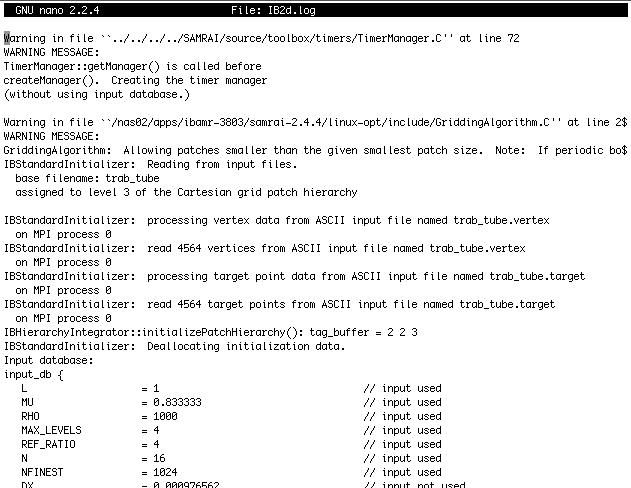
\includegraphics[width=0.95\linewidth]{x1-nano-ib2dlog-2014.png}

\vspace{1mm}

\includegraphics[width=0.95\linewidth]{x1-nano-shortcuts-2014.png}

\scriptsize \code{nano IB2d.log} on Kure (2014): the top of the log, and nano's shortcut bar.
\end{column}
\begin{column}{0.47\textwidth}
\footnotesize
\begin{itemize}\setlength{\itemsep}{2pt}
  \item \code{IB2d.log} reports, step by step, the time step, the simulation time, the Stokes solver's iterations and the CFL number.
  \item In nano: Ctrl+V a page down, Ctrl+Y a page up, Ctrl+W then Ctrl+V to the end and Ctrl+W then Ctrl+Y to the top (the notes write ``Ctrl + w + v''), Ctrl+X to leave, answering \code{n} to ``Save modified buffer?''.
  \item ``NOTE: For some reason as of August 2014, the nano editor cannot be used on Kill Devil, but it can be used on Kure.''
\end{itemize}
\vspace{1mm}
\al{Today}: nano on Puma (chapter 1); \code{tail -f} on the log while a job runs (chapter 3).
\end{column}
\end{columns}
\sourcecredit{Nick Battista, ``Party time in on super computers!'' (August 2014), pages 7--9 (Part I, steps 21--22 and the note after them), with his screenshots.}
\end{frame}

% 30
\begin{frame}{Following the log on the cluster (2/2): \code{vi}}
\label{fr:vi}
\begin{columns}[T,onlytextwidth]
\begin{column}{0.5\textwidth}
\centering
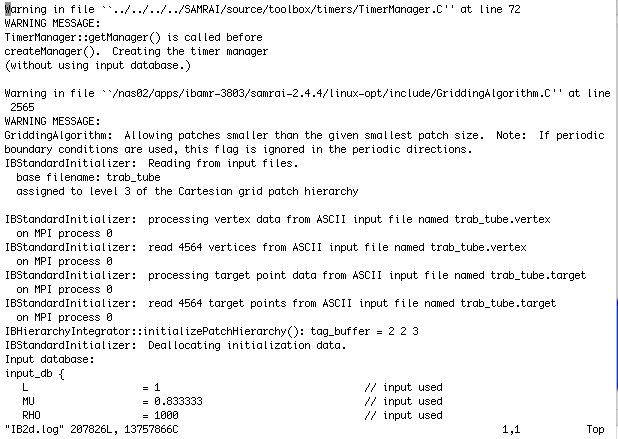
\includegraphics[width=0.8\linewidth]{x1-vi-ib2dlog-2014.png}

\vspace{1mm}
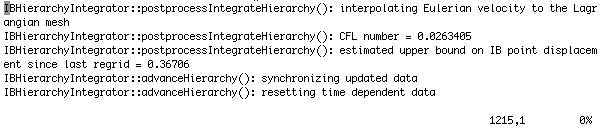
\includegraphics[width=0.95\linewidth]{x1-vi-line1215-2014.png}

\scriptsize \code{vi IB2d.log} (2014): the top of the file, and line 1215 after \code{:1215}.
\end{column}
\begin{column}{0.47\textwidth}
\footnotesize
\begin{itemize}\setlength{\itemsep}{2pt}
  \item \code{vi IB2d.log} opens the log; \code{:1215} jumps to line 1215 (the notes' example).
  \item \code{:wq} saves and quits, \code{:q} quits, \code{:q!} quits without saving.
  \item \al{A slip}: ``To make a change in vi \ldots\ hit the esc key. You can now write''. It is the other way round: \code{i} starts typing, Esc stops it, and the colon commands work after Esc.
\end{itemize}
\vspace{1mm}
\al{Today}: vi on Puma (chapter 1).
\end{column}
\end{columns}
\sourcecredit{Nick Battista, ``Party time in on super computers!'' (August 2014), pages 9--10 (Part I, step 24), with his screenshots; the vi slip is also in the 2018, 2020 and 2024 handouts.}
\end{frame}

% 31
\begin{frame}[fragile]{Getting results back (1/2): \code{tar} and \code{scp} (2014)}
\label{fr:results}
\begin{columns}[T,onlytextwidth]
\begin{column}{0.53\textwidth}
\hist{Dennis Evangelista's notes (2014), section 3.4}
\begin{lstlisting}[style=hist]
<onyen>@kure-login$ tar -cvzf viz_IB2d.tar.gz viz_IB2d/
<onyen>@kure-login$ exit
desktop$ scp <onyen>@kure.unc.edu:/netscr/<onyen>/FlowTank/viz_IB2d.tar.gz .
desktop$ tar -xvf viz_IB2d.tar.gz
desktop$ visit &
\end{lstlisting}
\hist{Nick Battista's notes (2014), as written}
\begin{lstlisting}[style=hist]
scp –r [your onyen]@kure.unc.edu:/netscr/[your onyen]/1st_Simulation Finished_Simulation
\end{lstlisting}
\end{column}
\begin{column}{0.44\textwidth}
\footnotesize
\begin{itemize}\setlength{\itemsep}{2pt}
  \item Copy the whole folder back ``at least within a week'' (\code{/netscr} ``recycles files''), to an external drive: 500 MB to 4 GB per simulation; data can be copied while the run is still going.
  \item One compressed file copies faster than thousands of small ones: \code{tar -cvzf} on the cluster, \code{tar -xvf} at home.
  \item Then VisIt on your own computer: \code{lag\_data.visit} for the structure, \code{dumps.visit} for the mesh, velocity and vorticity.
\end{itemize}
\vspace{1mm}
\al{Today}: \code{rsync} or \code{scp} from \code{/xdisk}, then remove what you copied (chapters 1 and 3).
\end{column}
\end{columns}
\sourcecredit{Dennis Evangelista's notes (2014), section 3.4 (prompts with placeholders); Nick Battista's notes (2014), part II (en dash as written).}
\end{frame}

% 31b
\begin{frame}[fragile]{Getting results back (2/2): a student's copy scripts}
\label{fr:results2}
\begin{columns}[T,onlytextwidth]
\begin{column}{0.55\textwidth}
\hist{``Running many simulations Part 2'' (2018), slides 19--20, condensed: comment lines and one \code{echo} line left out; user names and folders replaced}
\begin{lstlisting}[style=hist]
# This script downloads simulation results from KILLDEVIL cluster to my computer
echo "Downloading..."
scp -r <onyen>@killdevil.unc.edu:/netscr/<onyen>/<run_folder>/ /path/to/<results_folder>/

# Uploads <run_folder> to KILLDEVIL cluster from my computer
scp -r /path/to/<inputs_folder>/<run_folder> <onyen>@killdevil.unc.edu:/netscr/<onyen>/
\end{lstlisting}
\end{column}
\begin{column}{0.42\textwidth}
\footnotesize
\begin{itemize}\setlength{\itemsep}{2pt}
  \item Two short scripts, one \code{scp} line each (``The active line of code''), with comments that explain \code{scp} and \code{-r}, so that a run folder went up and its results came down with one command.
  \item Copying the run folder back whole brings the restart files and the logs with the pictures.
\end{itemize}
\vspace{1mm}
\al{Today}: the same scripts with \code{filexfer.hpc.arizona.edu} and \code{/xdisk/<pi>/<netid>}, or \code{rsync -av} (chapter 1).
\end{column}
\end{columns}
\sourcecredit{``7-IBAMR- Running many simulations Part 2'' (March 2018), slides 19--20: scripts by a student of the course (not named), with user names and folders replaced.}
\end{frame}


% 32
\begin{frame}[fragile]{3D runs on Kure and KillDevil}
\label{fr:kd3d}
\begin{columns}[T,onlytextwidth]
\begin{column}{0.48\textwidth}
\hist{``IBAMR Tutorial: UNC Edition'' (2014), slide 10}
\begin{lstlisting}[style=hist]
make clean
make main3d
bsub -q week -n 16 mpirun ./main3d input3d
\end{lstlisting}
\footnotesize ``this takes MUCH longer''.
\par\vspace{1mm}
\hist{TubeHeart ``Read me'' (February 2017)}
\begin{lstlisting}[style=hist]
These examples use a lot of memory. Please submit with this command
bsub -q week -n 32 -M 10 ./main3d input3d
\end{lstlisting}
\scriptsize No \code{mpirun}: LSF reserves 32 slots and one \code{main3d} runs (the Slurm case is slide \ref{fr:nompirun}). \code{-M} is LSF's memory limit (per process, unless the site made it per job); the note gives no unit, and LSF's default, KB, would make \code{-M 10} absurd for ``a lot of memory'', so UNC's unit was probably GB.
\end{column}
\begin{column}{0.49\textwidth}
\footnotesize
\begin{itemize}\setlength{\itemsep}{2pt}
  \item The same example built in 3D (\code{main3d}, \code{input3d}), on 16 processors; the 2012 notes recommend 16 to 32, ``powers of 2''.
  \item A 3D run could hold its cores for days in the \code{week} queue, LSF's longest.
  \item \code{make clean} came first ``for good measure'' (the 2012 notes); the Makefile itself cleaned the shared object files when the dimension changed, using its \code{stamp-2d} and \code{stamp-3d} markers (chapter X3).
\end{itemize}
\vspace{1mm}
\al{Today}: \code{main3d} is its own CMake target; a long run uses restarts (chapter 3).
\end{column}
\end{columns}
\sourcecredit{``IBAMR Tutorial: UNC Edition'' (2014), slide 10; the Miller lab's ReadMe deck (2012), slide 31; the TubeHeart ``Read me'' (2017).}
\end{frame}

% 32b
\begin{frame}[fragile]{Many runs at once under LSF (2018) (1/6): the plan and the template}
\label{fr:sweep1}
\begin{columns}[T,onlytextwidth]
\begin{column}{0.5\textwidth}
\footnotesize ``Goal'': run many simulations that vary parameters of \code{input2d}. Three pieces: a template \code{input2d}, a script \code{setinput2d.sh} that writes numbered input files, and a script that submits them all.

\vspace{1mm}
\code{allpara.txt}: three tab-separated columns, the Womersley number WO (changed through the viscosity), PAMP (the percent contraction, not used) and FREQ (the pumping frequency).
\par\vspace{1mm}
\hist{slide 4, ``template-input2d'', the lines that matter (tabs shown as spaces)}
\begin{lstlisting}[style=hist]
FRE = 1.25          //pumping frequency (Hz)
WO = 5.05           // desired Womersley number,original calculation
MU = 2.0*PI*FRE*RHO*D*D/(4.0*WO*WO)     // fluid dynamic viscosity (N s / m^2) to yield desired Wo, original calculation
\end{lstlisting}
\end{column}
\begin{column}{0.47\textwidth}
\scriptsize The template also sets \code{L = 1.0}, \code{D = 0.1}, \code{RHO = 1000.0}, \code{PI = 4.0*atan(1);} and keeps \code{//MU = 10}. Its output settings (slide 5): \code{viz\_writer = "VisIt"}, \code{viz\_dump\_interval = 1000}, \code{viz\_dump\_dirname = "viz\_IB2d"}, \code{visit\_number\_procs\_per\_file = 1}, \code{restart\_interval = 0}, \code{restart\_write\_dirname = "restart\_IB2d"}, \code{data\_dump\_interval = 0}, \code{data\_dump\_dirname = "hier\_data\_IB2d"}.

\vspace{2mm}
\footnotesize The viscosity is computed from the Womersley number, $\mathrm{Wo}^2 = \omega D^2/(4\nu)$ with $\omega = 2\pi f$ and $\nu = \mu/\rho$: setting WO and FRE sets MU. Chapter 3 quotes part of the generator and its three faults; these six slides keep the whole of it, as chapter 3 promises.
\end{column}
\end{columns}
\sourcecredit{The instructor's ``7-IBAMR- Running many simulations Part 2: Sample code'' (March 2018), slides 2--5.}
\end{frame}

% 32c
\begin{frame}[fragile]{Many runs at once under LSF (2018) (2/6): the generator, its start}
\label{fr:sweep2}
\begin{columns}[T,onlytextwidth]
\begin{column}{0.49\textwidth}
\hist{\code{setinput2d.sh}, slide 6}
\begin{lstlisting}[style=hist]
#!/bin/bash

# Separate main parameter file into three files
# Take the first column which lists the Womersley number (which is varied by changing viscosity).
cut -f 1 allpara.txt > Wo.txt
# Take the second column which lists the percent amplitude of contraction.
# cut -f 2 allpara.txt > pamp.txt
# Note that in this case the percent amplitude of contraction is not used.
# Take the third column which is the frequency.
cut -f 3 allpara.txt > Freq.txt
\end{lstlisting}
\end{column}
\begin{column}{0.48\textwidth}
\hist{slides 7--8}
\begin{lstlisting}[style=hist]
# Count number of lines in files
numlines=$(grep -c "^" allpara.txt)
# "^" basically reads a line that starts with anything (e.g. reads all lines).
# -c is an option to count.
# allpara.txt is the text files to read.

# initialize variables
WO=0
Freq=0

# For loop that will write files, count from 1 to the number of lines
for i in `seq 1 $numlines`;
do
\end{lstlisting}
\end{column}
\end{columns}
\sourcecredit{``7-IBAMR- Running many simulations Part 2: Sample code'' (March 2018), slides 6--8.}
\end{frame}

% 32c2
\begin{frame}[fragile]{Many runs at once under LSF (2018) (3/6): the loop sets WO and FRE}
\label{fr:sweep2b}
\hist{\code{setinput2d.sh}, slides 9--10 (inside the loop)}
\begin{lstlisting}[style=hist]
# Writes file to replace line with Wo
# Go to line 7 in template-input2d (which in the input2d template is the WO),
# Set that line to WO = "'"var"'"   // Womersley number
# Copy that file to input2dw${i}
awk -v var="$WO" 'NR==7 {$0="WO = "'"var"'"   // Womersley number"} 1' template-input2d > input2dw${i}

# Sets Freq based on i
# Read line i from the file Freq.txt and assign that value to Freq.
Freq=$(awk -v var="$i" 'NR==var' Freq.txt)
# Writes file to replace line with Freq
# Go to line 5 in the template, set that line to FRE = "'"var"'"   // Pumping Frequency (Hz)
# Copy that file to input2dw${i}f${i}
awk -v var="$Freq" 'NR==5 {$0="FRE = "'"var"'"   // Pumping Frequency (Hz)"} 1' input2dw${i} > input2dw${i}f${i}
\end{lstlisting}
\footnotesize Each \code{awk} line replaces one whole line of the input file, chosen by its number (\code{NR==7}, \code{NR==5}), and writes a new file. Freq is read from line \code{\$i} of \code{Freq.txt}; WO is not read at all (slide \ref{fr:sweep4}).
\sourcecredit{``7-IBAMR- Running many simulations Part 2: Sample code'' (March 2018), slides 9--10.}
\end{frame}

% 32d
\begin{frame}[fragile]{Many runs at once under LSF (2018) (4/6): log and output folders, and the run length}
\label{fr:sweep3}
\hist{\code{setinput2d.sh}, slides 11--12}
\begin{lstlisting}[style=hist]
# Edits input2d to create different IBlog and visit files and folders
awk -v var="$i" 'NR==201 {$0="   log_file_name = \"runs/IB2d.log"'"var"'"\"                //"} 1' input2dw${i}f${i} > input2dw${i}f${i}l${i}
awk -v var="$i" 'NR==207 {$0="   viz_dump_dirname = \"runs/viz_IB2d"'"var"'"\"                //"} 1' input2dw${i}f${i}l${i} > input2dw${i}f${i}l${i}y${i}

# The code below changes the simulation time based on the pumping frequency
test=$Freq
# echo $test
if [ $(echo " $test <= 0.70" | bc) -eq 1 ]
then
    cat template-input2d |  awk 'NR==24 {$0="END_TIME =      3.5                // Final Simulation Time (s)"} 1' input2dw${i}f${i}l${i}y${i} > input2dw${i}f${i}l${i}y${i}t${i}
elif [ $(echo " $test < 1.0" | bc) -eq 1 ]
then
    cat template-input2d |  awk 'NR==24 {$0="END_TIME =       3.0               // Final Simluation Time (s)"} 1' input2dw${i}f${i}l${i}y${i} > input2dw${i}f${i}l${i}y${i}t${i}
else
    cat template-input2d |  awk 'NR==24 {$0="END_TIME =       2.5                // Final Simulation Time (s)"} 1' input2dw${i}f${i}l${i}y${i} > input2dw${i}f${i}l${i}y${i}t${i}
fi
\end{lstlisting}
\footnotesize The run length follows the frequency: 3.5 s up to 0.70 Hz, 3.0 s below 1.0 Hz, 2.5 s otherwise, so that each run covers enough cycles.
\sourcecredit{``7-IBAMR- Running many simulations Part 2: Sample code'' (March 2018), slides 11--12.}
\end{frame}

% 32d2
\begin{frame}[fragile]{Many runs at once under LSF (2018) (5/6): the end of the loop}
\label{fr:sweep3b}
\hist{\code{setinput2d.sh}, slide 13; the closing \code{done} from slide 8}
\begin{lstlisting}[style=hist]
# Cleans up folder
rm input2dw${i} input2dw${i}f${i} input2dw${i}f${i}l${i} input2dw${i}f${i}l${i}y${i}
mv input2dw${i}f${i}l${i}y${i}t${i} input2d${i}

# Prints out END_TIME and FRE for a check
echo $i
grep "END_TIME =" input2d${i}  && grep "FRE ="  input2d${i}
done
\end{lstlisting}
\footnotesize Each step writes a new file named after the steps so far (\code{w}, \code{f}, \code{l}, \code{y}, \code{t}), and the last is renamed \code{input2d\$\{i\}}. The final \code{done} (slide 8, which shows the loop as \code{do} \ldots\ \code{done}) closes the loop opened on slide \ref{fr:sweep2}.
\sourcecredit{``7-IBAMR- Running many simulations Part 2: Sample code'' (March 2018), slide 13.}
\end{frame}

% 32e
\begin{frame}[fragile]{Many runs at once under LSF (2018) (6/6): submitting them, and the faults}
\label{fr:sweep4}
\begin{columns}[T,onlytextwidth]
\begin{column}{0.45\textwidth}
\hist{slide 14, ``Run simulations''}
\begin{lstlisting}[style=hist]
#!/bin/bash

startrun=31
endrun=40
mkdir parameters-files

# for i in "${!array}";
for i in `seq $startrun $endrun`;
do
   # run MPI program
   #Assumes all input2d files are in a folder called input2d-files
   bsub -q week -n 16 mpirun ./main2d input2d-files/input2d${i}
done
\end{lstlisting}
\end{column}
\begin{column}{0.52\textwidth}
\scriptsize \al{The faults} (chapter 3 points out the first three):
\begin{itemize}\setlength{\itemsep}{1.5pt}
  \item WO is never read from \code{Wo.txt} (there is no \code{WO=\$(awk ... Wo.txt)} line, as there is for Freq), so every file gets \code{WO = 0} and the formula for MU divides by zero.
  \item The generator writes \code{input2d\$\{i\}} in the current folder; the runner reads \code{input2d-files/input2d\$\{i\}}; the \code{parameters-files} folder it makes is never used.
  \item Fixed line numbers (\code{NR==7}, \code{5}, \code{201}, \code{207}, \code{24}) break silently when the template changes.
  \item Neither script makes the \code{runs/} folder named in the log and visualization lines; runs 31--40 are hard-coded; \code{cat template-input2d |} before an \code{awk} that reads a named file does nothing; ``Simluation''.
\end{itemize}
\vspace{1mm}
\footnotesize \al{Today}: replace values by name and submit a Slurm job array (chapter 3).
\end{column}
\end{columns}
\sourcecredit{``7-IBAMR- Running many simulations Part 2: Sample code'' (March 2018), slide 14; the faults checked against slides 6--14 (October 2026).}
\end{frame}


% 33
\begin{frame}{The first-simulation handouts (1/2): UNC, 2014--2018}
\label{fr:handouts}
\scriptsize
\renewcommand{\arraystretch}{1.12}
\setlength{\tabcolsep}{3pt}
\begin{tabular}{@{}L{0.09\textwidth}L{0.27\textwidth}L{0.13\textwidth}L{0.13\textwidth}L{0.13\textwidth}L{0.17\textwidth}@{}}
\toprule
date & handout & machine & IBAMR & runs with & runs in \\
\midrule
May 2014 & ``Using IBAMR Module on Kure - Instructions for Undergraduates'' & Kure, KillDevil & \code{ibamr/3803} & \code{bsub -n 2} & \code{/netscr/\allowbreak onyen} \\
May 2014 & Dennis Evangelista's notes & Kure & \code{ibamr/3803} & \code{bsub -n 2} & \code{/netscr/\allowbreak <onyen>} \\
May 2014, Jan 2015 & ``IBAMR Tutorial: UNC Edition'' (MATH 769, Lecture 3) & Kure & \code{ibamr/3803} & \code{bsub -n 2} & \code{/netscr/\allowbreak <onyen>} \\
Aug 2014 & Nick Battista, ``Party time in on super computers!'' & Kure, KillDevil & \code{ibamr/3803} (in its log) & \code{bsub -n 8} & \code{/netscr/\allowbreak <onyen>} \\
2017--18 & ``Getting Started on UNC cluster'' & KillDevil & \code{ibamr/\allowbreak 2016-11} & \code{bsub -n 2} & \code{/netscr/\allowbreak <onyen>} \\
Jan 2018 & ``1 - Get killdevil account and software'' (the account and software steps) & KillDevil & -- & -- & -- \\
Jan 2018 & ``Run your first IBAMR simulation'' (adapted from the 2014 notes) & KillDevil & \code{ibamr/\allowbreak 2016-11} & \code{bsub -n 8} & \code{/netscr/\allowbreak <onyen>} \\
\bottomrule
\end{tabular}
\sourcecredit{The handouts named in the table.}
\end{frame}

% 33b
\begin{frame}{The first-simulation handouts (2/2): 2018--2026}
\label{fr:handouts2}
\scriptsize
\renewcommand{\arraystretch}{1.12}
\setlength{\tabcolsep}{3pt}
\begin{tabular}{@{}L{0.09\textwidth}L{0.27\textwidth}L{0.13\textwidth}L{0.13\textwidth}L{0.13\textwidth}L{0.17\textwidth}@{}}
\toprule
date & handout & machine & IBAMR & runs with & runs in \\
\midrule
Apr 2018 & ``2-Run your IBAMR simulation on Dogwood'' & Dogwood & \code{ibamr/\allowbreak 2018-03} & \code{sbatch} & \code{/21dayscratch/\allowbreak ...} \\
May 2020 & ``Get dogwood account and run a simulation'' (adapted again) & Dogwood & \code{ibamr/\allowbreak 2018-03} & \code{sbatch} & \code{/21dayscratch/\allowbreak ...} \\
July 2024 & ``Get HPC account and run a simulation'' (UA Lecture 1) & Puma, Ocelote, El Gato & a group install & \code{sbatch} & \code{/xdisk/\allowbreak <group>/<netid>} \\
2025--26 & this series, chapters 1--3 & Puma & autoibamr & \code{sbatch job.\allowbreak slurm} & \code{/xdisk/\allowbreak <pi>/<netid>} \\
\bottomrule
\end{tabular}

\vspace{2mm}
\footnotesize One handout, rewritten for each machine: the 2014 text survives into 2020 with ``killdevil'' and ``netscr'' left in a Dogwood guide, and the 2020 guide still shows the 2014 Kure screenshots. The May 2014 Kure guide is the source of the home, module, \code{/netscr} and \code{bsub} slides of the Kure deck of the same month, which links to it, and the 2018 KillDevil and Dogwood notes are the sources of the 2020 guide. Each change of machine changed four lines: the host, the IBAMR module, the scheduler command and the scratch folder.
\sourcecredit{The handouts named in the table.}
\end{frame}

% 34
\begin{frame}{The FlowTank first run (2014)}
\label{fr:flowtank}
\begin{columns}[T,onlytextwidth]
\begin{column}{0.47\textwidth}
\scriptsize
\begin{itemize}\setlength{\itemsep}{2pt}
  \item The May 2014 notes started everyone on one example, the flow tank: a channel ``10x10x20 cm with parabolic inflow and outflow'', with a triangle (2D) or a cone (3D) held in place by target points; its \code{.vertex} and \code{.target} files came from \code{generate\_mesh2d.m} and \code{generate\_mesh3d.m}.
  \item \code{FlowTank.zip} was uploaded to \code{/netscr/<onyen>}, built and submitted as on the last slides; the results came back as \code{viz\_IB2d} (the deck says ``viz2d (or viz3d)'') for VisIt.
  \item In VisIt: \code{lag\_data.visit} for the Lagrangian points, \code{dumps.visit} (the deck also writes ``Dump.visit'') for the Eulerian fields; Add, Vector, U and Add, Pseudocolor, Omega; Add, Mesh, \code{cones2d\_512\_vertices} for the triangle's points.
\end{itemize}
\vspace{1mm}
\al{Today}: IB/03 (a tethered beam in a channel) and IBFE/10 (a plate in a 3D flow tank); VisIt is chapters 26--27.
\end{column}
\begin{column}{0.5\textwidth}
\centering
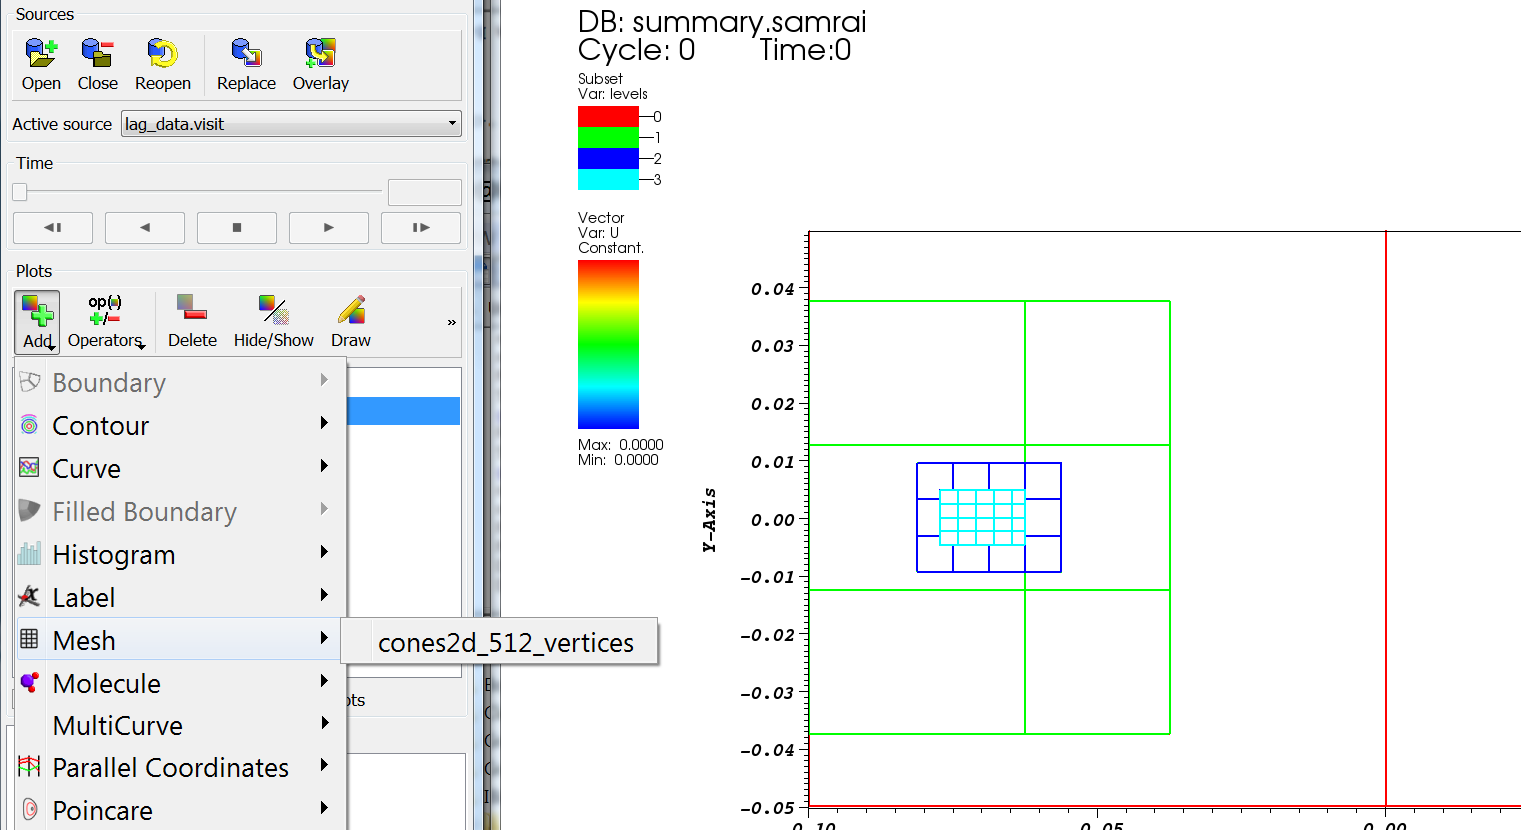
\includegraphics[width=\linewidth]{x1-flowtank-visit-2014.png}

\scriptsize VisIt 2.x (2014): adding the triangle's points as a Mesh plot over the patch levels of the flow tank.
\end{column}
\end{columns}
\sourcecredit{``IBAMR Tutorial: UNC Edition'' (May 2014), slides 7--8 and 13--17, with its screenshot (slide 17); Dennis Evangelista's notes (2014), section 3.2.}
\end{frame}

% 35
\begin{frame}[fragile]{IB2d on Kure and KillDevil (2016)}
\label{fr:ib2dkure}
\begin{columns}[T,onlytextwidth]
\begin{column}{0.48\textwidth}
\hist{``Getting Running on IB2D and IBAMR'' (2016), slide 2}
\begin{lstlisting}[style=hist]
# "Ssh into kure. Cd into the directory where you want to
#  download ib2d. In the command window type:"
module add git/1.8.5.3
git clone https://github.com/nickabattista/IB2d.git
\end{lstlisting}
\hist{IB talk (2016), page 67, ``How to run IB2d''}
\begin{lstlisting}[style=hist]
ssh [your-onyen]@kure.unc.edu
module load matlab
# change to the example folder; edit input2d
bmatlab main2d.m
\end{lstlisting}
\end{column}
\begin{column}{0.49\textwidth}
\footnotesize
\begin{itemize}\setlength{\itemsep}{2pt}
  \item IB2d, Nick Battista's MATLAB and Python immersed boundary code, ran on the clusters as a MATLAB batch job (next slide); \code{git} itself was a module.
  \item Output: the flow and Lagrangian positions in \code{viz\_IB2d}; ``Force data is in the \code{hier\_IB2d\_data} folder''. (The IBAMR examples' folder of the same deck is \code{hier\_data\_IB2d}: two programs, two names; both are right.)
  \item ``Be sure to module add ibamr/3803. May not work if matlab module is loaded'' for IBAMR on the same machines (slide \ref{fr:clashes}).
\end{itemize}
\vspace{1mm}
\al{Today}: \code{git clone} on Puma with no module, MATLAB as a module in a job script (chapter 1); IB2d itself is Part II.
\end{column}
\end{columns}
\sourcecredit{``Getting Running on IB2D and IBAMR'' (MATH 768, 2016), slides 2--4, 7 and 9; IB talk by Nick Battista and Laura A. Miller (7 September 2016), page 67.}
\end{frame}

% 36
\begin{frame}[fragile]{MATLAB jobs under LSF: \code{bmatlab}}
\label{fr:bmatlab}
\begin{columns}[T,onlytextwidth]
\begin{column}{0.52\textwidth}
\hist{``Getting Running on IB2D and IBAMR'' (2016), slides 5--6}
\begin{lstlisting}[style=hist]
module add matlab
# with a window (from your computer):
ssh -X onyen@kure.unc.edu
module add matlab
xmatlab
# a serial batch job:
bmatlab matlabjob.m
# or the same job with bsub, on one line:
bsub matlab -nodisplay -nosplash -singleCompThread -r matlabjob -logfile matlabjob.out
\end{lstlisting}
\end{column}
\begin{column}{0.45\textwidth}
\footnotesize
\begin{itemize}\setlength{\itemsep}{2pt}
  \item \code{bmatlab} was a UNC script that submitted a MATLAB file as a one-core LSF job, ``the easiest way to submit a serial Matlab job'' on Kure and KillDevil.
  \item With \code{bsub matlab ... -r matlabjob} the \code{.m} is left off the file name after \code{-r}; the output goes to \code{matlabjob.out} in the working folder.
  \item \code{ssh -X} forwarded MATLAB's window to your own screen (\code{xmatlab}).
\end{itemize}
\vspace{1mm}
\al{Today}: a Slurm script with \code{module load matlab} and \code{matlab -nodisplay -nosplash < main2d.m} (chapter 1).
\end{column}
\end{columns}
\sourcecredit{``Getting Running on IB2D and IBAMR'' (2016), slides 5--6 (paraphrasing UNC's help pages of the time); the IB talk (2016), page 67.}
\end{frame}

% 37
\begin{frame}[fragile]{Module clashes the notes warned about}
\label{fr:clashes}
\begin{columns}[T,onlytextwidth]
\begin{column}{0.5\textwidth}
\scriptsize
\begin{itemize}\setlength{\itemsep}{3pt}
  \item 2014: ``You must first remove any other module'' before \code{module add ibamr/3803}; ``You may also need to delete manually in your .profile, .bashrc, and .bash\_profile files in your home directory'' (the \code{initadd} lines).
  \item 2016, IBAMR and MATLAB: ``Be sure to module add ibamr/3803. May not work if matlab module is loaded.''
  \item 2016, VisIt: ``You will want to module rm ibamr/3803 as there is a conflict''; then \code{module add visit}.
  \item 2017--18, VisIt with the 2016-11 module: \code{module rm ibamr/2016-11} before \code{module add visit/2.12.3} (next slides).
  \item The likely cause: each module put its own libraries first on the library path (HDF5, Python, compilers), and two modules wanted different versions.
\end{itemize}
\end{column}
\begin{column}{0.47\textwidth}
\hist{``Analyzing your IBFE simulation'' (2018), slide 8, condensed}
\begin{lstlisting}[style=hist]
[<onyen>@killdevil-login2 ~]$ module list
  1) git/1.8.5.3  2) openmpi_gcc/4.8.1  3) python/2.6.5  4) ibamr/2016-11
[<onyen>@killdevil-login2 ~]$ module rm ibamr/2016-11
[<onyen>@killdevil-login2 ~]$ module add visit/2.12.3
\end{lstlisting}
\footnotesize \al{Today}: load only what a job needs, in the job script itself; a VisIt job loads \code{visit} and nothing of IBAMR's (chapter 31).
\end{column}
\end{columns}
\sourcecredit{``IBAMR Killdevil Module'' (2014), slide 2; ``Getting Running on IB2D and IBAMR'' (2016), slides 9--10; ``Analyzing your IBFE simulation'' (2018), slide 8; ``Visit from command line and Python'' (2018), slide 3.}
\end{frame}

% 38
\begin{frame}{VisIt on KillDevil (1/3): the modules}
\label{fr:visitkd}
\begin{columns}[T,onlytextwidth]
\begin{column}{0.55\textwidth}
\footnotesize
\begin{itemize}\setlength{\itemsep}{2pt}
  \item Two VisIt modules: \code{visit} (VisIt 2.5.2) and \code{visit/2.12.3}. Scripts had to match: ``record your python commands in visit 2.5.2. You can use later versions of visit, but you may need to debug your code. This older version of visit may also be incompatible with the newest Mac OS.''
  \item ``Warning to user! The visit installed on killdevil cannot read .ex2 files. You will need to download the .ex2 files, export them as .vtk files, and then create a script that reads in vtk.''
  \item With a window: ``If you ssh -X into killdevil, typing visit then brings up the GUI.''
  \item Paths recorded on a laptop or desktop (\code{/Users/<user>/Desktop/...}) had to be changed to the cluster's (\code{localhost:/nas/...}) before a script ran there: ``I recommend doing a search to find all paths.''
\end{itemize}
\end{column}
\begin{column}{0.42\textwidth}
\begin{punchbox}
\small \al{Today}: Puma's \code{visit} module is VisIt 3.4.2, or your own VisIt 3.5.0; VisIt 3 reads ExodusII files, and VisIt 3.2 and later run Python 3 scripts (chapter 31).
\end{punchbox}
\end{column}
\end{columns}
\sourcecredit{``Resampling AMR grids'' (2017--18), slide 2; ``Analyzing your IBFE simulation'' (2018), slides 6, 9 and 15; ``Getting Running on IB2D and IBAMR'' (2016), slide 10.}
\end{frame}

% 39
\begin{frame}[fragile]{VisIt on KillDevil (2/3): scripts without a window}
\label{fr:visitcli}
\begin{columns}[T,onlytextwidth]
\begin{column}{0.52\textwidth}
\hist{``Visit from command line and Python'' (2018), slide 3, condensed}
\begin{lstlisting}[style=hist]
[<onyen>@killdevil-login1 <run_folder>]$ module rm ibamr/2016-11
[<onyen>@killdevil-login1 <run_folder>]$ module add visit/2.12.3
[<onyen>@killdevil-login1 <run_folder>]$ visit -cli -nowin
Running: cli2.5.2 -nowin
Running: viewer2.5.2 -host 127.0.0.1 -port 5600 -noint -nowin
Python 2.6.4 (r264:75706, Aug 23 2012, 13:48:37)
[GCC Intel(R) C++ gcc 4.1 mode] on linux2
>>> Source("heart_script.py")
\end{lstlisting}
\hist{slide 4, ``Alternative method (easier)''}
\begin{lstlisting}[style=hist]
[<onyen>@killdevil-login1 <run_folder>]$ visit -cli -nowin -s heart_script.py
Running: cli2.12.3 -nowin -s heart_script.py
Running: viewer2.12.3 -nowin -noint -host 127.0.0.1 -port 5600
Running: mdserver2.12.3 -host 127.0.0.1 -port 5600
Running: engine_ser2.12.3 -host 127.0.0.1 -port 5600
\end{lstlisting}
\end{column}
\begin{column}{0.45\textwidth}
\footnotesize
\begin{itemize}\setlength{\itemsep}{2pt}
  \item \code{visit -cli -nowin} runs VisIt's Python interface with no window; \code{Source()} runs a recorded script inside it, and \code{-s} runs it from the command line.
  \item \al{A puzzle in the transcript}: after \code{module add visit/2.12.3} the first run reports VisIt 2.5.2 (the default module's), the second 2.12.3. The 2017 resampling deck (slide 17) has the same transcript after \code{module add visit}, the 2.5.2 default: the 2018 slide most likely edited the module line of that older transcript.
  \item Both ran on the login node, as the notes did then.
\end{itemize}
\vspace{1mm}
\al{Today}: \code{visit -cli -nowin -s script.py} with the full path, in a batch job (chapter 31).
\end{column}
\end{columns}
\sourcecredit{``Visit from command line and Python'' (2018), slides 1--4 (prompts with placeholders; the script name as on the slide).}
\end{frame}

% 40
\begin{frame}[fragile]{VisIt on KillDevil (3/3): building your own (2018)}
\label{fr:visitbuild}
\begin{columns}[T,onlytextwidth]
\begin{column}{0.5\textwidth}
\hist{``Visit from command line and Python'' (2018), slides 7--10, condensed}
\begin{lstlisting}[style=hist]
# get build_visit2_12_3 (VisIt 2.12.3 releases page)
# put it in e.g. $HOME/sfw/visit
chmod 755 build_visit2_12_3
./build_visit2_12_3 --mesa        # answer "yes"
# then, in the visit2.12.3/src folder:
make package
# untar, then install:
svn_bin/visit-install VERSION ARCH INSTALL_DIR_PATH
svn_bin/visit-install 2_12_3 linux-x86_64 $HOME/sfw/visit_12_2_3
# run without the GUI:
cd $HOME/sfw/visit_12_2_3/bin
./visit -cli -nowin
\end{lstlisting}
\end{column}
\begin{column}{0.47\textwidth}
\scriptsize
\begin{itemize}\setlength{\itemsep}{2pt}
  \item Your own VisIt 2.12.3 (the version of the \code{visit/2.12.3} module; the default \code{visit} was 2.5.2), built from source with \code{build\_visit} and Mesa (software rendering, for a machine with no screen), then installed with \code{visit-install}.
  \item \al{Slips}: the heading says ``Install your own version of visit (dogwood)'' over KillDevil steps; the version argument is written \code{2\_12\_3}, where \code{visit-install} expects \code{2.12.3}, and the install folder \code{visit\_12\_2\_3} transposes the version (harmless, but confusing); the slides print a full home path with a user name (replaced here by \code{\$HOME}).
  \item The rest of the deck (recording scripts in the Commands window, saving frames in a loop) is chapters 31--32.
\end{itemize}
\vspace{1mm}
\al{Today}: a VisIt release for Rocky Linux 9, installed with \code{visit-install} (chapter 31).
\end{column}
\end{columns}
\sourcecredit{``Visit from command line and Python'' (2018), slides 7--10 (home paths replaced; the steps condensed, the commands as written).}
\end{frame}

% 41
\begin{frame}{When a job ``finished'' in a second, and other KillDevil troubles}
\label{fr:kdtroubles}
\begin{columns}[T,onlytextwidth]
\begin{column}{0.52\textwidth}
\begin{homebox}
\footnotesize ``the parallelization has been sort of buggy recently\ldots if you submit a job and it finishes within a fraction of a second\ldots the simulation DID NOT finish\ldots try resubmitting the job OR run it on a single node, e.g., change to a 1'' (September 2016): that is \code{-n 1}, one process.
\end{homebox}
\vspace{1mm}
\footnotesize The other troubles of the notes: the \code{libimf.so} error of the 3803 module (slide \ref{fr:m3803}); module clashes (slide \ref{fr:clashes}); \code{nano} not working on KillDevil in August 2014 (slide \ref{fr:nano}); a home path that ``was messed up'' in a Makefile (slide \ref{fr:a4make}); \code{/netscr} files vanishing after 21 days (slide \ref{fr:netscr}).
\end{column}
\begin{column}{0.45\textwidth}
\footnotesize
\begin{itemize}\setlength{\itemsep}{2pt}
  \item A job that ends at once has failed at start-up: a missing library, a bad input line, an MPI launch problem. When resubmitting helped, the failure was probably in a node, not in the job.
  \item The first thing to read is the job's output and error file; LSF e-mailed a summary.
\end{itemize}
\vspace{1mm}
\al{Today}: read the \code{.out} file and \code{sacct}; chapter 3 lists the common first errors, and chapter 16 the ones that come later.
\end{column}
\end{columns}
\sourcecredit{IB talk by Nick Battista and Laura A. Miller (7 September 2016), page 75; the slides named.}
\end{frame}

% 42
\begin{frame}{Kure and KillDevil, then and now}
\label{fr:kkthennow}
\scriptsize
\renewcommand{\arraystretch}{1.12}
\setlength{\tabcolsep}{4pt}
\begin{tabular}{@{}L{0.2\textwidth}L{0.36\textwidth}L{0.38\textwidth}@{}}
\toprule
 & Kure, KillDevil (2012--2018) & Puma (2025--26; chapters 1--3) \\
\midrule
account & ONYEN Services, ``subscribe to services'' & HPC portal; a PI sponsors you into their group \\
log in & \code{ssh <onyen>@kure.unc.edu} (VPN off campus) & \code{ssh <netid>@hpc.arizona.edu}, then \code{shell} (no VPN for SSH) \\
run folder & \code{/netscr/<onyen>}, 21 days & \code{/xdisk/<pi>/<netid>}, 150 days (+150) \\
software & \code{module initadd ibamr/3803} (or \code{2016-11}) & autoibamr in your home; \code{module load gnu13 openmpi5}; \code{enable.sh} \\
build & a Makefile with \code{IBAMR\_SRC\_DIR}; \code{make main2d} on the login node & CMake; build in an \code{interactive} session or a job \\
submit & \code{bsub -q week -n 8 mpirun ./main2d input2d} & \code{sbatch job.slurm} with \code{mpirun -np "\$SLURM\_NTASKS"} \\
watch, stop & \code{bjobs}, \code{bkill} & \code{squeue --me}, \code{scancel}, \code{sacct} \\
log & \code{nano} or \code{vi IB2d.log} & the log and \code{.out} file, \code{tail -f} \\
results & \code{tar}, \code{scp} back within a week & \code{rsync} or \code{scp}; \code{/groups} or your own drive \\
VisIt & modules 2.5.2 and 2.12.3; no ExodusII & module 3.4.2 or your own 3.5.0 \\
\bottomrule
\end{tabular}
\sourcecredit{This part of the chapter; chapters 1--3 and 31.}
\end{frame}

% 43
\begin{frame}{Dogwood and Longleaf at a glance (2018--2020)}
\label{fr:dwglance}
\begin{columns}[T,onlytextwidth]
\begin{column}{0.55\textwidth}
\footnotesize
\begin{itemize}\setlength{\itemsep}{1.5pt}
  \item \al{Two UNC clusters after KillDevil}, sharing a home folder and a software tree (\code{/nas/longleaf/...}): Dogwood, built for large parallel jobs that talk across many nodes (the course's IBAMR runs), and Longleaf, for data-heavy work on one node at a time (the lecture's COMSOL run, for instance).
  \item \al{The scheduler was Slurm}: ``Dogwood uses the SLURM cluster management and scheduling software'' (2018; the 2019--20 lecture made it ``Dogwood/longleaf'' and added a note for the course: ``*killdevil used LSF'').
  \item IBAMR came as a module again: \code{ibamr/2018-03} (March 2018), then \code{ibamr/0.6.0} (June 2020).
  \item \al{Storage}: scratch folders (\code{/21dayscratch} on Dogwood, emptied after 21 days; \code{/pine/scr} on Longleaf, whose clean-up the notes do not state), a home folder, and mass storage (\code{\textasciitilde/ms}, up to 1 TB) for keeping results.
\end{itemize}
\end{column}
\begin{column}{0.42\textwidth}
\begin{punchbox}
\small The course slides of 2018--20 copied their descriptions from UNC's Research Computing pages; this chapter rewrites them. Puma today plays both roles: one cluster for parallel IBAMR runs and for single-node work (chapter 1).
\end{punchbox}
\end{column}
\end{columns}
\sourcecredit{``2-Run your IBAMR simulation on Dogwood'' (April 2018), slides 2 and 4, repeated with Longleaf added in Lecture 8, ``COMSOL workflow, export and run remotely'' (2019--20), slides 18 and 20; ``Get dogwood account and run a simulation'' (2020); the course Makefiles' comments; IBFE lecture 5 (June 2020). Retirement dates are not stated in the course's files.}
\end{frame}

% 43a
\begin{frame}{Where the Dogwood notes came from}
\label{fr:dwsources}
\small
\begin{itemize}\setlength{\itemsep}{3pt}
  \item \al{January 2018}: ``1 - Get killdevil account and software'' gave the account and software steps; by May 2020 they were the Dogwood guide's steps 1--7 (the guide's Drive copy dates from November 2019), with ``killdevil'' changed to ``dogwood'' in most places.
  \item \al{April 2018}: ``2-Run your IBAMR simulation on Dogwood'' (27 slides; created April 2018, edited until May 2020) introduced Dogwood, Slurm, the \code{ibamr/2018-03} module and the first job scripts; it also holds the debugging tips (slides 13--16), added on a date not recorded. It is the original of the Slurm slides that the 2019--20 COMSOL lecture repeats (slides 18--26 of that lecture are its slides 2--10, with Longleaf added).
  \item \al{July 2019}: ``Debugging Tips'', the same tips (= slides 13--16 of the 2018 deck; made in three minutes, so a copy; slide \ref{fr:dwdebug}).
  \item \al{November 2019 -- May 2020}: ``Get dogwood account and run a simulation'', revised in May 2020 for the online summer series.
\end{itemize}
\vspace{2mm}
\footnotesize So the Slurm material of the next slides comes from a deck begun in April 2018, even where it is quoted from a later copy.
\sourcecredit{The course files' Drive dates and line-by-line comparisons (October 2026).}
\end{frame}


% 44
\begin{frame}{Getting a Dogwood account (2020)}
\label{fr:dwaccount}
\begin{columns}[T,onlytextwidth]
\begin{column}{0.55\textwidth}
\scriptsize
\begin{itemize}\setlength{\itemsep}{2pt}
  \item ONYEN Services, ``Subscribe to Services'', Dogwood. The page could answer: ``You are ineligible for the following services \ldots\ KillDevil Cluster: missing \code{'(LIVE|EXCH)'} prerequsite'' [\emph{sic}].
  \item If it did, an e-mail to UNC Research Computing saying so, with: your ONYEN, your UNC e-mail address, full name, campus address, a campus phone and a number where you can be reached while running jobs, department, your faculty sponsor's (PI's) name and ONYEN if known, and a description of the work; and ``do not request to be added to a group''.
  \item These steps are the January 2018 KillDevil handout's, with ``killdevil'' changed to ``dogwood'' in most places (slide \ref{fr:dwsources}).
  \item The guide of May 2020 then installs the desktop tools: an SSH program (Mac Terminal or PuTTY, port 22), VPN, FileZilla, VisIt, a plain-text editor, MATLAB.
\end{itemize}
\end{column}
\begin{column}{0.42\textwidth}
\begin{punchbox}
\small \al{Today}: the UA HPC portal, a PI group that sponsors you, and the group's allocation on Puma (chapter 1). Personal details go to the university's forms, never into shared notes.
\end{punchbox}
\end{column}
\end{columns}
\sourcecredit{``Get dogwood account and run a simulation'' (the instructor, May 2020; its second part adapted from Nick Battista's 2014 notes), Step 1 and Steps 2--7; ``1 - Get killdevil account and software'' (January 2018).}
\end{frame}

% 45
\begin{frame}{Off campus: VPN and Duo (2019--20)}
\label{fr:dwvpn}
\begin{columns}[T,onlytextwidth]
\begin{column}{0.55\textwidth}
\small
\begin{itemize}\setlength{\itemsep}{3pt}
  \item From off campus, the VPN client first, then \code{ssh} or FileZilla; the 2018 slides (repeated in the 2019 lecture) warned that a Cisco client already set up for another VPN ``may not let you switch between the two''.
  \item With it came Duo, UNC's two-step login on a phone.
  \item The May 2020 guide pointed to UNC's VPN help page and the campus software site for the client.
\end{itemize}
\end{column}
\begin{column}{0.42\textwidth}
\begin{punchbox}
\small \al{Today}: no VPN for SSH or Open OnDemand at Arizona; two-step login (Duo) at the bastion host; the HPC VPN only for programs that cannot pass the bastion (chapter 1).
\end{punchbox}
\end{column}
\end{columns}
\sourcecredit{``2-Run your IBAMR simulation on Dogwood'' (2018), slide 3 = Lecture 8 (2019--20), slide 19; ``Get dogwood account and run a simulation'' (2020), Step 3 and Part I, item 9.}
\end{frame}

% 46
\begin{frame}[fragile]{Storage on Dogwood and Longleaf}
\label{fr:dwstorage}
\begin{columns}[T,onlytextwidth]
\begin{column}{0.5\textwidth}
\hist{2019--20 lecture and 2020 guide (\code{<onyen>} for the user ID)}
\begin{lstlisting}[style=hist]
# Dogwood scratch (run here; emptied after 21 days)
cd /21dayscratch/scr/o/n/<onyen>/
# Longleaf scratch
/pine/scr/o/n/<onyen>
# Longleaf home
/nas/longleaf/home/<onyen>
# mass storage in your home: up to 1 TB
cd ~/ms
\end{lstlisting}
\end{column}
\begin{column}{0.47\textwidth}
\footnotesize
\begin{itemize}\setlength{\itemsep}{2pt}
  \item In \code{scr/o/n/<onyen>}, \code{o} and \code{n} stand for the first two letters of your ONYEN.
  \item ``whatever you put in this directory is erased after 21 days''; move results to mass storage, ``preferably in tar or zip format''.
  \item Mass storage (\code{\textasciitilde/ms}): ``Do not run programs out of this directory.''
  \item \al{Leftovers} in the 2020 guide: ``To run simulations we must change directories to our netscr directory'' (KillDevil's folder) before the Dogwood path.
\end{itemize}
\vspace{1mm}
\al{Today}: \code{/xdisk/<pi>/<netid>} for runs; results to your own computer or an external drive; \code{/groups/<pi>} for the group's shared files (chapter 1).
\end{column}
\end{columns}
\sourcecredit{``2-Run your IBAMR simulation on Dogwood'' (2018), slides 2 and 4 (with Longleaf added in Lecture 8, 2019--20, slides 18 and 20); ``Get dogwood account and run a simulation'' (2020), pages on storage; G. Hobson's 2020 VisIt tutorial (the Longleaf home).}
\end{frame}

% 47
\begin{frame}[fragile]{Moving files to and from Dogwood}
\label{fr:dwscp}
\begin{columns}[T,onlytextwidth]
\begin{column}{0.53\textwidth}
\hist{``Get dogwood account and run a simulation'' (2020), as written}
\begin{lstlisting}[style=hist]
scp –r 1st_Simulation [your onyen]@dogwood.unc.edu: /21dayscratch/scr/o/n/onyen
scp –r [your onyen]@dogwood.unc.edu:/21dayscratch/scr/o/n/[your onyen]/1st_Simulation Finished_Simulation
\end{lstlisting}
\hist{the first line, as it should read}
\begin{lstlisting}[style=hist]
scp -r 1st_Simulation <onyen>@dogwood.unc.edu:/21dayscratch/scr/o/n/<onyen>
\end{lstlisting}
\end{column}
\begin{column}{0.44\textwidth}
\footnotesize
\begin{itemize}\setlength{\itemsep}{2pt}
  \item The 2014 commands with the new host and scratch path, and two slips: the en dash in \code{\ndashmark{}r}, and a space after the colon, which makes the scratch path a separate argument: \code{scp} then takes it as the destination on your own computer, and the remote home folder as a second source.
  \item FileZilla works too; the guide's heading still says ``SFTP (moving files between local computer and killdevil)''.
  \item Copy back ``at least within a week'', to an external drive (the 2014 advice, unchanged).
\end{itemize}
\vspace{1mm}
\al{Today}: \code{scp}, \code{rsync} or FileZilla to \code{filexfer.hpc.arizona.edu} (chapter 1).
\end{column}
\end{columns}
\sourcecredit{``Get dogwood account and run a simulation'' (2020), Step 4, Part I (item 15) and Part II (en dashes and placeholders as written).}
\end{frame}

% 48
\begin{frame}[fragile]{The Dogwood IBAMR modules: \code{2018-03} and \code{0.6.0}}
\label{fr:dwmodules}
\begin{columns}[T,onlytextwidth]
\begin{column}{0.5\textwidth}
\hist{2020 guide (prompt scrubbed)}
\begin{lstlisting}[style=hist]
[<onyen>@dogwood-login1 769_examples]$ module add ibamr/2018-03
[<onyen>@dogwood-login1 769_examples]$ module list
Currently Loaded Modules:
  1) openmpi_2.0.3/gcc_4.8.5   2) ibamr/2018-03
\end{lstlisting}
\hist{IBFE lecture 5, ``Plans for June'' (1 June 2020), slide 3}
\begin{lstlisting}[style=hist]
To load the old module:
module add ibamr
module list
Currently Loaded Modules:
 1) openmpi_2.0.3/gcc_4.8.5   2) ibamr/2018-03
To load the new module
module add ibamr/0.6.0
module list
Currently Loaded Modules:
  1) openmpi_2.0.3/gcc_4.8.5   2) ibamr/0.6.0
To remove a module
module rm ibamr
\end{lstlisting}
\end{column}
\begin{column}{0.47\textwidth}
\scriptsize
\begin{itemize}\setlength{\itemsep}{2pt}
  \item ``There is now a new ibamr install on dogwood (as of this morning). I will update all of the examples for that install over the next month. WARNING: I have not tested this yet!''
  \item ``I recommend installing your own updated version of ibamr as well''; the old examples were to be kept in a folder \code{ibamr-examples-2018-03} (none survives in the course's files). The reasons given for moving: two-boundary IBFE handling had changed, and the constraint-IB and sharp-interface methods were only in the new install.
  \item ``Any example without a date appended on the end is for the 2016-11 version of IBAMR to run on killdevil. These examples will NOT run on dogwood.'' The updated ones were ``appended with 2018-03'' (2018).
  \item The Makefile lines for both modules are in chapter X3 (dating code by its paths).
\end{itemize}
\vspace{1mm}
\al{Today}: no IBAMR module on Puma: your own autoibamr build (chapter 2).
\end{column}
\end{columns}
\sourcecredit{``2-Run your IBAMR simulation on Dogwood'' (2018), slides 11 and 20; ``Get dogwood account and run a simulation'' (2020); IBFE lecture 5, ``Plans for June'' (1 June 2020), slides 2--4.}
\end{frame}

% 49
\begin{frame}{Slurm on Dogwood: \code{sbatch}, \code{squeue}, \code{scancel}}
\label{fr:slurmdw}
\begin{columns}[T,onlytextwidth]
\begin{column}{0.55\textwidth}
\small
\begin{itemize}\setlength{\itemsep}{3pt}
  \item \code{sbatch script.sh} submits a job script; Slurm answers with the job's number.
  \item \code{squeue -u <onyen>} lists your jobs (``provide your onyen to just show your jobs''); the 2018 slide prints \code{squeue -u} with the name left out, and the 2020 guide writes \code{squeue -uonyen}, with the placeholder to replace.
  \item \code{scancel [JobID]} stops one.
  \item The commands are the same today; what changed is the partition names, the account line, and the way the program is launched inside the script.
\end{itemize}
\end{column}
\begin{column}{0.42\textwidth}
\begin{punchbox}
\small \al{Today}: \code{squeue --me}, \code{scancel <jobid>}, \code{sacct} for jobs that have ended (chapter 1).
\end{punchbox}
\end{column}
\end{columns}
\sourcecredit{``2-Run your IBAMR simulation on Dogwood'' (2018), slides 4--5 (with Longleaf added in Lecture 8, 2019--20, slides 20--21); ``Get dogwood account and run a simulation'' (2020).}
\end{frame}

% 50
\begin{frame}[fragile]{A first Slurm script, twice}
\label{fr:firstslurm}
\begin{columns}[T,onlytextwidth]
\begin{column}{0.32\textwidth}
\hist{Lecture 8 (2019--20), slides 22--23 (in the deck begun in April 2018)}
\begin{lstlisting}[style=hist]
nano example.sh

#!/bin/bash
#SBATCH --job-name=first_slurm_job
#SBATCH --ntasks=1
#SBATCH --time=1:00
#SBATCH --mem=100
echo "Hello SLURM"

sbatch example.sh
\end{lstlisting}
\end{column}
\begin{column}{0.32\textwidth}
\hist{2020 guide}
\begin{lstlisting}[style=hist]
#!/bin/bash
#SBATCH --job-name=first_slurm_job
#SBATCH --ntasks-per-node=16
#SBATCH --time=1:00:00
#SBATCH --mem=1000
echo "Hello SLURM"
\end{lstlisting}
\end{column}
\begin{column}{0.32\textwidth}
\footnotesize
\begin{itemize}\setlength{\itemsep}{2pt}
  \item ``each SBATCH switch below has two `-' characters''.
  \item The lecture's script asks for ``1 core and 100MB of memory for 1 minute'', as its text says (\code{--time=1:00} is one minute, \code{--mem=100} is in MB).
  \item The 2020 guide changed the script (16 tasks per node, one hour, 1000 MB) but kept the old sentence: the text no longer matches.
\end{itemize}
\end{column}
\end{columns}
\vspace{1mm}
\footnotesize \al{Today}: chapter 1's first job script names the account and partition, asks for memory per core, and is checked with \code{squeue --me}.
\sourcecredit{``2-Run your IBAMR simulation on Dogwood'' (2018), slides 6--7 = Lecture 8 (2019--20), slides 22--23; ``Get dogwood account and run a simulation'' (2020).}
\end{frame}

% 51
\begin{frame}[fragile]{One-line jobs: \code{sbatch --wrap}, and Slurm's defaults on Longleaf}
\label{fr:wrap}
\begin{columns}[T,onlytextwidth]
\begin{column}{0.5\textwidth}
\hist{Lecture 8 (2019--20), slide 24}
\begin{lstlisting}[style=hist]
$ sbatch -t 1 -n 1 -o hello.out --wrap="echo hello SLURM"
\end{lstlisting}
\footnotesize The defaults the slide lists: partition \code{general} (\code{-p}), one task (\code{-n 1}), \code{--mem-per-cpu=4800} (MB), and a one-hour limit, written \code{-t 60}, \code{-t 1:00:00}, \code{-t 0-01:00} or \code{--time=1:00:00}; \code{-t 1-0} is one day.
\end{column}
\begin{column}{0.47\textwidth}
\footnotesize
\begin{itemize}\setlength{\itemsep}{2pt}
  \item \code{--wrap} turns one command into a job without writing a script; \code{-o} names the output file.
  \item \al{A slip} in slide 26's example (a Python job on another group's path): ``Time = 1 hour'' for \code{-t 1}, which is one \emph{minute} (a bare number is minutes), and ``Number nodes = 1'' for \code{-n 1}, which counts \emph{tasks}.
\end{itemize}
\vspace{1mm}
\al{Today}: \code{--wrap} works on Puma too, once \code{--account} and \code{--partition} are added (chapter 1); a script is easier to keep and to repeat.
\end{column}
\end{columns}
\sourcecredit{``2-Run your IBAMR simulation on Dogwood'' (2018), slides 8 and 10 = Lecture 8 (2019--20), slides 24 and 26 (the slide 26 path is a third party's, not reproduced).}
\end{frame}

% 52
\begin{frame}[fragile]{Shortcuts: \code{showqueue} and \code{deletealljobs}}
\label{fr:aliases}
\begin{columns}[T,onlytextwidth]
\begin{column}{0.52\textwidth}
\hist{Lecture 8 (2019--20), slide 25, as written}
\begin{lstlisting}[style=hist]
alias showqueue='squeue -u YOUR_ONYEN'
alias deletealljobs='scancel -u YOUR_ONYEN’
\end{lstlisting}
\footnotesize ``showqueue is basically the command: bjobs''; ``deletealljobs is basically the command: bkill 0''.
\end{column}
\begin{column}{0.45\textwidth}
\footnotesize
\begin{itemize}\setlength{\itemsep}{2pt}
  \item Two aliases, typed at the prompt or kept in \code{\textasciitilde/.bashrc}, gave the old LSF habits new names.
  \item \al{A slip}: the second line closes with a curly quote (\code{’}), so the shell keeps waiting for the closing \code{'}.
\end{itemize}
\vspace{1mm}
\al{Today}: \code{alias showqueue='squeue -u \$USER'}, or simply \code{squeue --me}; \code{scancel -u \$USER} stops all your jobs (chapter 3).
\end{column}
\end{columns}
\sourcecredit{``2-Run your IBAMR simulation on Dogwood'' (2018), slide 9 = Lecture 8, ``COMSOL workflow, export and run remotely'' (2019--20), slide 25.}
\end{frame}

% 53
\begin{frame}[fragile]{The IBAMR job script on Dogwood (1/2): the 2020 scripts}
\label{fr:dwjob}
\begin{columns}[T,onlytextwidth]
\begin{column}{0.48\textwidth}
\hist{2020 guide, the first IBAMR job}
\begin{lstlisting}[style=hist]
#!/bin/bash
#SBATCH --job-name=first_ibamr_job
#SBATCH --ntasks-per-node=16
#SBATCH --time=2:00:00
#SBATCH --mem=1000
#SBATCH --partition=debug_queue
#SBATCH --output IBFE2D.out
mpirun ./main2d input2d
\end{lstlisting}
\hist{the course's 2D examples (\code{examples/legacy}), e.g.\ the rubber band}
\begin{lstlisting}[style=hist]
#!/bin/bash
#SBATCH --job-name=ibamr-rubberband
#SBATCH --ntasks-per-node=16
#SBATCH --time=2:00:00
#SBATCH --partition=debug_queue
#SBATCH --output ibamr2d.out

mpirun ./main2d input2d
\end{lstlisting}
\end{column}
\begin{column}{0.49\textwidth}
\footnotesize
\begin{itemize}\setlength{\itemsep}{2pt}
  \item 16 tasks on one node, two hours, the \code{debug\_queue} partition; \code{mpirun} with no count takes every task Slurm gave the job.
  \item ``there are a number of partitions to which you can submit. Some have minimum numbers of ntasks and run times'' (UNC's partition table).
  \item The other 2D course scripts follow it, with their own job names (\code{ibamr-pulsatile}, \code{ibamr-leaf}, \code{ibamr-cylinders}, \code{ibamr-spring}, \code{ibamr-2plates}); the 3D glycocalyx asks for the same 16 tasks and runs \code{main3d}.
\end{itemize}
\vspace{1mm}
\al{Today}: chapter 3's \code{job.slurm}: \code{--account}, \code{--partition=standard}, \code{--ntasks=4}, \code{--mem-per-cpu}, the modules, \code{enable.sh}, \code{mpirun -np "\$SLURM\_NTASKS"}.
\end{column}
\end{columns}
\sourcecredit{``Get dogwood account and run a simulation'' (2020); the job scripts of \code{examples/legacy/UNC-Examples} (2020).}
\end{frame}

% 53b
\begin{frame}[fragile]{The IBAMR job script on Dogwood (2/2): the first one, April 2018}
\label{fr:dwjob2018}
\begin{columns}[T,onlytextwidth]
\begin{column}{0.47\textwidth}
\hist{``Run your IBAMR simulation on Dogwood'' (2018), slide 12, ``Sample 2D script''}
\begin{lstlisting}[style=hist]
#!/bin/bash
#SBATCH --job-name=first_ibfe_job
#SBATCH --ntasks=64
#SBATCH --time=2:00:00
#SBATCH --mem=1000
#SBATCH --partition=528_queue
#SBATCH --output IBFE2D.out

mpirun ./main2d input2d
\end{lstlisting}
\end{column}
\begin{column}{0.5\textwidth}
\footnotesize
\begin{itemize}\setlength{\itemsep}{2pt}
  \item 64 tasks in the \code{528\_queue} partition for a 2D example: Dogwood's large-job partitions had a minimum size, and smaller jobs waited with the reason \code{QOSMinCpuNotSatisfied} (slide \ref{fr:dwdebug}).
  \item \code{--mem=1000} is 1000 MB per node in total, for all the tasks on it; the 2019 tips raise it to \code{--mem=50000}.
  \item The 2020 scripts (last slide) moved to \code{debug\_queue} with 16 tasks per node.
\end{itemize}
\vspace{1mm}
\al{Today}: \code{--mem-per-cpu}, and as many tasks as the run needs (chapter 3).
\end{column}
\end{columns}
\sourcecredit{The instructor's ``2-Run your IBAMR simulation on Dogwood'' (created April 2018), slide 12.}
\end{frame}


% 54
\begin{frame}[fragile]{Scripts that forgot \code{mpirun}}
\label{fr:nompirun}
\begin{columns}[T,onlytextwidth]
\begin{column}{0.47\textwidth}
\hist{the course's IBFE examples 1-, 2- and 4- (2020)}
\begin{lstlisting}[style=hist]
#!/bin/bash
#SBATCH --job-name=first_ibfe_job
#SBATCH --ntasks=16
#SBATCH --time=2:00:00
#SBATCH --partition=debug_queue
#SBATCH --output IBFE2D.out

./main2d input2d
\end{lstlisting}
\end{column}
\begin{column}{0.5\textwidth}
\begin{homebox}
\footnotesize The script reserves 16 tasks but starts the program directly, not through \code{mpirun}: \al{one process runs, and 15 reserved cores sit idle} for the whole job. Nothing fails, so nothing warns you: the run takes as long as a one-core run, with 15 cores reserved and unused.
\end{homebox}
\vspace{1mm}
\footnotesize The IBFE examples 7- and 9- (built with \code{ibamr/0.6.0}) have \code{mpirun}.

\vspace{1mm}
\al{Today}: \code{mpirun -np "\$SLURM\_NTASKS" ./build/main2d input2d} (chapter 3).
\end{column}
\end{columns}
\sourcecredit{The job scripts of \code{examples/legacy/UNC-Examples} (1-, 2-, 4-, 7- and 9-series IBFE folders, 2020).}
\end{frame}

% 55
\begin{frame}[fragile]{Big 3D jobs: \code{528\_queue}, and restarts}
\label{fr:528}
\begin{columns}[T,onlytextwidth]
\begin{column}{0.48\textwidth}
\hist{the course's 3D IBFE examples (2020)}
\begin{lstlisting}[style=hist]
#!/bin/bash
#SBATCH --job-name=528_queue
#SBATCH --ntasks-per-node=32
#SBATCH -N 2
#SBATCH --time=72:00:00
#SBATCH --partition=528_queue
#SBATCH --output IBFE3D.out

mpirun ./main3d input3d
\end{lstlisting}
\hist{G. Hobson's tutorial (2020), slide 30, ``Restarting a job''}
\begin{lstlisting}[style=hist]
#!/bin/bash
#SBATCH --job-name=re48
#SBATCH --ntasks-per-node=44
#SBATCH -N 4
#SBATCH --time=72:00:00
#SBATCH --partition=528_queue
#SBATCH --output output

mpirun ./main3d input3d $PWD/restart_IB3d 995000
\end{lstlisting}
\end{column}
\begin{column}{0.49\textwidth}
\footnotesize
\begin{itemize}\setlength{\itemsep}{2pt}
  \item Dogwood's \code{528\_queue} partition took the big parallel jobs: here 2 nodes of 32 tasks (64 cores) for up to 72 hours. The job name repeats the partition's name, harmlessly.
  \item A run longer than the time limit continues from a restart file: the restart folder and the step number follow the input file on the command line (here step 995000, on 4 nodes of 44 tasks).
  \item A restart must use the same number of processes as the run that wrote it.
\end{itemize}
\vspace{1mm}
\al{Today}: restarts work the same way on Puma (chapter 3); a long run is split into jobs within the partition's time limit.
\end{column}
\end{columns}
\sourcecredit{The 3D job scripts of \code{examples/legacy/UNC-Examples} (horseshoe crab, flow tank, two wings; 2020); Gabrielle Hobson, ``Post-Processing IBAMR Simulation Data in VisIt on a Computing Cluster'' (23 September 2020), slide 30.}
\end{frame}

% 56
\begin{frame}{Watching a Dogwood job}
\label{fr:dwwatch}
\begin{columns}[T,onlytextwidth]
\begin{column}{0.55\textwidth}
\small
\begin{itemize}\setlength{\itemsep}{3pt}
  \item Keep a record of each job: its number, what it was, its parameters (the 2014 advice, kept).
  \item \code{squeue -uonyen} (with your ONYEN) while it waits and runs.
  \item The run's log, \code{IB2d.log}, read with \code{nano} or \code{vi} as in 2014 (slides \ref{fr:nano}--\ref{fr:vi}); the guide keeps the 2014 slip about Esc in vi.
  \item ``Please see lecture 1 for how to visualize this data!''
\end{itemize}
\end{column}
\begin{column}{0.42\textwidth}
\begin{punchbox}
\small \al{Today}: \code{squeue --me}; \code{tail -f} on the log; \code{sacct -j <jobid>} after the job; the job's \code{.out} file for errors (chapters 1 and 3).
\end{punchbox}
\end{column}
\end{columns}
\sourcecredit{``Get dogwood account and run a simulation'' (2020), the sections on watching and copying a job.}
\end{frame}

% 56b
\begin{frame}[fragile]{When a Dogwood job waits, stops or crawls}
\label{fr:dwdebug}
\begin{columns}[T,onlytextwidth]
\begin{column}{0.53\textwidth}
\scriptsize ``The number of nodes requested can freeze your job'': ``I submitted a bunch of jobs on Dogwood, but they are all pending with the code (QOSMinCpuNotSatisfied).'' ``Solution: You need to make sure you are above the minimum number of nodes you must request.''
\par\vspace{0.5mm}
\hist{``My job randomly stopped''}
\begin{lstlisting}[style=hist]
Look at the end of both the IB2d.log / IB3d.log files to see what happened.
Also look at the .out file to see if what happened. This file is named after whatever you put in your script.
PETSC errors happen if you did not dedicate enough memory.
In your script, increase the mem option:
#SBATCH --mem=50000
You may not have devoted enough time in your job.
In your script, increase the time option
#SBATCH --time=4:00:00
\end{lstlisting}
\hist{``My job is super slow''}
\begin{lstlisting}[style=hist]
IBAMR can trip up if you use the wrong number of nodes (too many  nodes, or some weird number).
Try to make the number of nodes a power of 2.
2D simulations can really slow down if you use too many nodes.
Make sure your DT isn’t too small in the input file.
\end{lstlisting}
\end{column}
\begin{column}{0.44\textwidth}
\scriptsize
\begin{itemize}\setlength{\itemsep}{2pt}
  \item ``nodes'' here means MPI processes (tasks); the pending reason is about the number of CPUs a partition requires.
  \item A PETSc error is one possible sign of too little memory, not the only cause; \code{--mem=50000} is 50{,}000 MB (about 49 GB) per node.
  \item ``A power of 2'' is a habit, not a rule; too many processes for a small 2D run does slow it down.
\end{itemize}
\vspace{1mm}
\al{Today}: chapter 3's table of first errors and chapter 16's list of slow and failing runs are these tips, rewritten for Puma.
\end{column}
\end{columns}
\sourcecredit{The instructor's ``2-Run your IBAMR simulation on Dogwood'' (2018--20), slides 13--16, and ``Debugging Tips'' (July 2019), the same text.}
\end{frame}


% 57
\begin{frame}[fragile]{Longleaf: a COMSOL batch run (2019)}
\label{fr:comsol}
\begin{columns}[T,onlytextwidth]
\begin{column}{0.53\textwidth}
\hist{Lecture 8 (2019--20), slide 17, the log condensed}
\begin{lstlisting}[style=hist]
module load comsol/5.4
# the COMSOL batch log (Tue Feb 19 2019):
#   COMSOL 5.3a (Build: 348) opening
#   /nas/longleaf/home/<onyen>/COMSOL/Barnacle.mph
File created with a later version of COMSOL Multiphysics. - Version: COMSOL 5.4.0.225
\end{lstlisting}
\end{column}
\begin{column}{0.44\textwidth}
\footnotesize
\begin{itemize}\setlength{\itemsep}{2pt}
  \item The lecture ran a COMSOL model (heat in a barnacle) as a batch job on Longleaf, the single-node cluster.
  \item ``NOTE: module load comsol/5.4'': the log shows COMSOL 5.3a refusing a file saved with 5.4, so the job had run the wrong version. Load the version the file was saved with.
  \item COMSOL itself is outside this series; the lesson carries over to any program with modules: name the version.
\end{itemize}
\end{column}
\end{columns}
\sourcecredit{Lecture 8, ``COMSOL workflow, export and run remotely'' (2019--20), slide 17 (the user ID replaced).}
\end{frame}

% 58
\begin{frame}[fragile]{VisIt on Dogwood and Longleaf (2020) (1/2): installing it yourself}
\label{fr:visitdw}
\begin{columns}[T,onlytextwidth]
\begin{column}{0.53\textwidth}
\hist{G. Hobson's tutorial (2020), slides 4--5}
\begin{lstlisting}[style=hist]
cd ~
mkdir visit
cd visit
scp visit3_1_2.linux-x86_64-rhel7-wmesa.tar.gz <onyen>@dogwood.unc.edu:~/visit/
 tar -xvf visit3_1_2.linux-x86_64-rhel7-wmesa.tar.gz
/nas/longleaf/home/<onyen>/visit/visit3_1_2.linux-x86_64/bin/visit -cli -nowin -s script.py
\end{lstlisting}
\footnotesize The download: VisIt 3.1.2, ``the last option'' on the executables page, a Red Hat Enterprise Linux 7.5 build that ``Includes Mesa support for rendering without a display''.
\end{column}
\begin{column}{0.44\textwidth}
\footnotesize
\begin{itemize}\setlength{\itemsep}{2pt}
  \item Download on your computer, \code{scp} to the cluster, unpack, and run by its full path: no module and no build.
  \item On the slides the command is written with en dashes (\code{\ndashmark{}cli \ndashmark{}nowin \ndashmark{}s}, in red), which VisIt does not read as options; the full-path line is right.
  \item A message at start-up, that the ADIOS2 database plugin could not load a library, is harmless: that one reader is missing, the others work.
\end{itemize}
\vspace{1mm}
\al{Today}: the same recipe for Puma, with a current VisIt for Rocky Linux 9 (chapter 31).
\end{column}
\end{columns}
\sourcecredit{Gabrielle Hobson, ``Post-Processing IBAMR Simulation Data in VisIt on a Computing Cluster'' (Scripps Institution of Oceanography, UCSD; 23 September 2020), slides 3--5 and 15--16 (the user ID replaced).}
\end{frame}

% 59
\begin{frame}[fragile]{VisIt on Dogwood and Longleaf (2/2): paths in the scripts}
\label{fr:visitpaths}
\begin{columns}[T,onlytextwidth]
\begin{column}{0.54\textwidth}
\hist{G. Hobson's tutorial (2020), slide 10 (paths with placeholders; the correlation lines left out)}
\begin{lstlisting}[style=hist]
string_dumps = "localhost:/nas/longleaf/home/<onyen>/code/rubber_band/viz_IB2d/dumps.visit"
string_mesh = "localhost:/nas/longleaf/home/<onyen>/code/rubber_band/viz_IB2d/lag_data.visit"
string_output = "/21dayscratch/scr/<o>/<n>/<onyen>/flow_fields/rubber_band"
OpenDatabase(string_dumps)
OpenDatabase(string_mesh)
\end{lstlisting}
\scriptsize
\begin{itemize}\setlength{\itemsep}{2pt}
  \item A script recorded on a laptop or desktop has that computer's paths; on the cluster each must become \code{localhost:} plus the cluster's path. Slide 9 of the tutorial has the slips (a missing colon after \code{localhost}, a curly quote, a missing opening quote); slide 10 is right.
  \item ``commands to do with `spontaneous states', like when you click the zoom icon in the GUI, do not work on the cluster''.
  \item VisIt 3.1 on the cluster ``has trouble reading .VTK databases'': the tutorial copies a \code{dumps.visit} into the VTK folder and lists the \code{.vtk} files in it.
\end{itemize}
\end{column}
\begin{column}{0.43\textwidth}
\centering
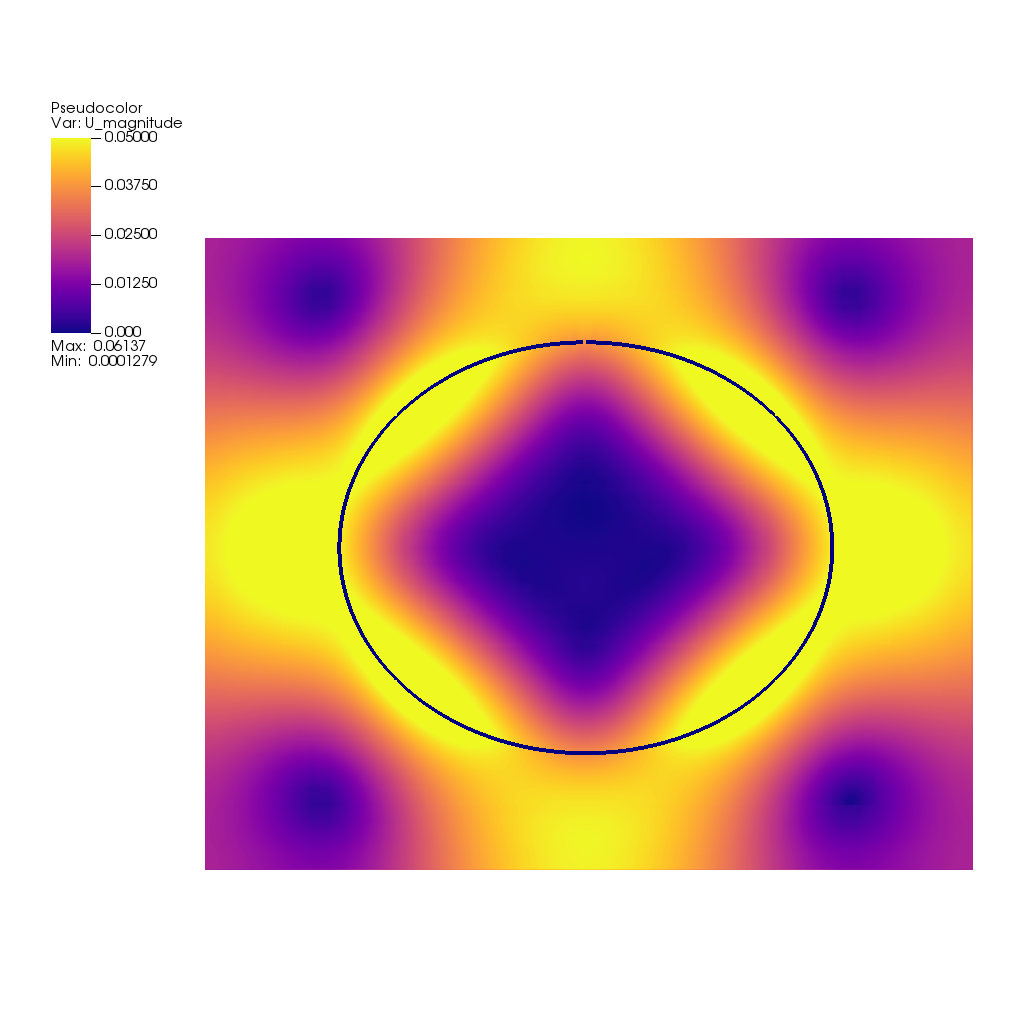
\includegraphics[width=0.8\linewidth]{x1-hobson-rubberband-frame-2020.png}

\scriptsize A frame of the rubber band rendered on the cluster with no display (the tutorial's figure).
\vspace{1mm}

\footnotesize \al{Today}: chapter 31 (paths, batch rendering, VTK series opened directly in VisIt 3.5).
\end{column}
\end{columns}
\sourcecredit{Gabrielle Hobson, ``Post-Processing IBAMR Simulation Data in VisIt on a Computing Cluster'' (2020), slides 9--10, 13, 17 (her figure), 20 and 24.}
\end{frame}

% 60
\begin{frame}{Dogwood and Longleaf, then and now}
\label{fr:dwthennow}
\scriptsize
\renewcommand{\arraystretch}{1.12}
\setlength{\tabcolsep}{4pt}
\begin{tabular}{@{}L{0.2\textwidth}L{0.37\textwidth}L{0.37\textwidth}@{}}
\toprule
 & Dogwood, Longleaf (2018--2020) & Puma (2025--26; chapters 1--3) \\
\midrule
account & ONYEN Services, or an e-mail to Research Computing & HPC portal, sponsored by a PI group \\
log in & \code{ssh <onyen>@dogwood.unc.edu}; VPN and Duo off campus & \code{ssh <netid>@hpc.arizona.edu}, Duo, then \code{shell} \\
run folder & \code{/21dayscratch/scr/o/n/<onyen>} (21 days) & \code{/xdisk/<pi>/<netid>} (150 days, +150) \\
keep & \code{\textasciitilde/ms}, up to 1 TB & \code{/groups/<pi>}, 500 GB; your own drive \\
software & \code{module add ibamr/2018-03} or \code{ibamr/0.6.0} & autoibamr; \code{module load gnu13 openmpi5}; \code{enable.sh} \\
job script & \code{--ntasks-per-node=16}, \code{--partition=debug\_queue} or \code{528\_queue}; \code{mpirun ./main2d input2d} & \code{--account}, \code{--partition=standard}, \code{--ntasks=4}; \code{mpirun -np "\$SLURM\_NTASKS"} \\
watch, stop & \code{squeue -u <onyen>}, \code{scancel} & \code{squeue --me}, \code{scancel}, \code{sacct} \\
VisIt & your own 3.1.2 (RHEL 7, Mesa) by its full path & module 3.4.2 or your own 3.5.0 \\
\bottomrule
\end{tabular}
\sourcecredit{This part of the chapter; chapters 1--3 and 31.}
\end{frame}

% 61
\begin{frame}{UArizona's clusters, 2021--2024: Puma, Ocelote, El Gato}
\label{fr:uaglance}
\begin{columns}[T,onlytextwidth]
\begin{column}{0.5\textwidth}
\footnotesize
\begin{itemize}\setlength{\itemsep}{0pt}
  \item Three clusters behind one bastion host: Puma (the newest), Ocelote and El Gato. ``After you login to the bastion host, select puma or ocelot''; ``Once connected, you are using a login node'', and ``software is not available on the login nodes''.
  \item Puma and Ocelote used Slurm (``Uses SLURM scheduling software'', 2022), and by 2023 El Gato was a third Slurm target. Ocelote moved to Slurm in June--July 2021 (the banner on the right; the July 2021 slides expected it ``online July 12''); no source in the course's files uses Ocelote's earlier scheduler.
  \item The notes call Ocelote ``ocelot'' throughout; the shortcut at the bastion was \code{ocelote}.
  \item El Gato was shut down on 29 July 2026 and Ocelote on 17 August 2026; since then Puma is the only UA cluster (chapter 1).
\end{itemize}
\end{column}
\begin{column}{0.47\textwidth}
\centering
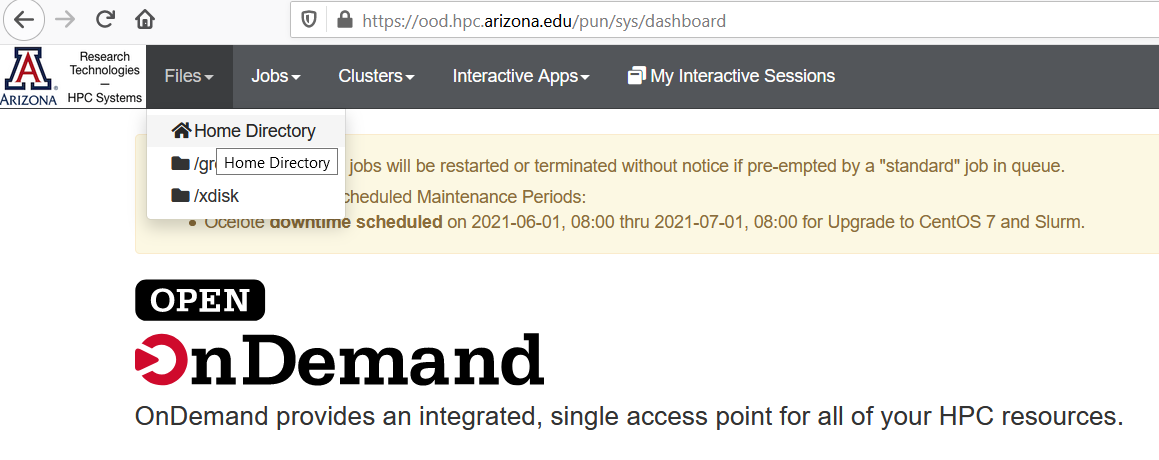
\includegraphics[width=\linewidth]{x1-ood-banner-2021.png}

\scriptsize Open OnDemand at Arizona, spring 2021: windfall jobs ``will be restarted or terminated without notice if pre-empted by a `standard' job''; ``Ocelote downtime scheduled on 2021-06-01, 08:00 thru 2021-07-01, 08:00 for Upgrade to CentOS 7 and Slurm.''
\end{column}
\end{columns}
\sourcecredit{``HPC and computing resources @ UA'' (about 2022), slides 21 and 29, and the screenshot of the OnDemand dashboard on its slide 24 (spring 2021); ``HPC @ UA, running ib2d and IBAMR'' (2021--22); chapter 1 for the 2026 shutdowns.}
\end{frame}

% 62
\begin{frame}{Accounts and groups (2021--2024)}
\label{fr:uaaccount}
\begin{columns}[T,onlytextwidth]
\begin{column}{0.55\textwidth}
\footnotesize
\begin{itemize}\setlength{\itemsep}{2pt}
  \item 2021--22: request HPC on the university's account page (``Manage your Accounts'', High Performance Computing); ``I will need to add you to my group''.
  \item ``Note that there is a charge for simulations -- please use the windfall partition unless you have permission for standard.'' And in OnDemand: ``if you select Standard, your PI will be charged for the time. Although windfall is not recommended, it is free and can be used for low risk tasks.''
  \item 2024: the account at the HPC portal (\code{portal.hpc.arizona.edu}) with a sponsorship request to the PI.
\end{itemize}
\end{column}
\begin{column}{0.42\textwidth}
\begin{punchbox}
\small \al{Today}: the portal and a PI sponsor as in 2024; \code{standard} jobs use the PI group's allocation of CPU hours (\code{--account=<your PI group>}), \code{windfall} is free and can be pre-empted (chapter 1).
\end{punchbox}
\end{column}
\end{columns}
\sourcecredit{``HPC @ UA, running ib2d and IBAMR'' (2021--22), slides 3--4; ``HPC and computing resources @ UA'' (about 2022), slides 17 and 27; UA Lecture 1 (July 2024).}
\end{frame}

% 63
\begin{frame}[fragile]{Choosing a cluster at the bastion}
\label{fr:bastion}
\begin{columns}[T,onlytextwidth]
\begin{column}{0.5\textwidth}
\hist{UA notes, 2021--2024 (\code{<netid>} for the user ID)}
\begin{lstlisting}[style=hist]
ssh <netid>@hpc.arizona.edu
# two-step login, then at the bastion host:
puma        # or ocelote, or elgato
\end{lstlisting}
\footnotesize ``you are currently logged into the Bastion Host. You must now log into puma, ocelot, or elgato. on the cluster. Let's log into puma.'' (2024)
\end{column}
\begin{column}{0.47\textwidth}
\footnotesize
\begin{itemize}\setlength{\itemsep}{2pt}
  \item The bastion host (\code{hpc.arizona.edu}) is only a gateway: a cluster's name typed there opened a login node, and by 2023 the same names were shortcuts that ``change the target cluster'' for jobs.
  \item The 2021--22 slides say ``Type puma/ocelot to work on this cluster''.
\end{itemize}
\vspace{1mm}
\al{Today}: \code{ssh <netid>@hpc.arizona.edu}, then \code{shell} (Puma is the only cluster; chapter 1).
\end{column}
\end{columns}
\sourcecredit{UA Lecture 1 (July 2024), the login section (its screenshot of the shortcut list retyped); ``HPC @ UA, running ib2d and IBAMR'' (2021--22), slides 10 and 16.}
\end{frame}

% 64
\begin{frame}{VPN and two-step login, 2021--2024}
\label{fr:uavpn}
\begin{columns}[T,onlytextwidth]
\begin{column}{0.55\textwidth}
\small
\begin{itemize}\setlength{\itemsep}{3pt}
  \item 2021--22: the Cisco VPN client to \code{vpn.arizona.edu} from off campus, with a second password of \code{push} or \code{phone} for Duo.
  \item 2024: ``Please install the cisco client''.
  \item FileZilla and \code{sftp} asked for the NetID password and then \code{1} for a Duo push (or a passcode).
\end{itemize}
\end{column}
\begin{column}{0.42\textwidth}
\begin{punchbox}
\small \al{Today}: no VPN for SSH or Open OnDemand; Duo at the bastion host; the HPC VPN (\code{vpn.hpc.arizona.edu}) only for programs that cannot pass the bastion (chapter 1).
\end{punchbox}
\end{column}
\end{columns}
\sourcecredit{``HPC @ UA, running ib2d and IBAMR'' (2021--22), slides 6--8; ``HPC and computing resources @ UA'' (about 2022), slides 4 and 19; UA Lecture 1 (2024).}
\end{frame}

% 65
\begin{frame}[fragile]{Moving files, 2021--2024: FileZilla, \code{sftp}, OnDemand}
\label{fr:uafiles}
\begin{columns}[T,onlytextwidth]
\begin{column}{0.5\textwidth}
\hist{``HPC @ UA'' (2021--22), slides 9--10}
\begin{lstlisting}[style=hist]
# from the folder on your computer:
sftp <netid>@filexfer.hpc.arizona.edu
# "Once logged in, type puma or ocelot to use one of these servers"
put file
put -r folder
get file
get -r folder
\end{lstlisting}
\footnotesize FileZilla: protocol SFTP, host \code{filexfer.hpc.arizona.edu}, logon type Interactive, user your NetID; in the Transfer Settings, a limit of 1 connection (one Duo approval per connection).
\end{column}
\begin{column}{0.47\textwidth}
\footnotesize
\begin{itemize}\setlength{\itemsep}{2pt}
  \item Open OnDemand's file browser (\code{ood.hpc.arizona.edu}): drag and drop.
  \item \al{Slips}: a slide on the university's general server writes \code{sftp netid@uarizona.edu} for \code{u.arizona.edu} (as the same slide says three lines earlier); ``a terminal that allows 2-step authentication (Cygwin for PC, terminal for Mac)'' : Cygwin was not needed; Windows' own \code{ssh} (PowerShell, Windows Terminal), WSL or PuTTY do this (chapter 1).
  \item The \code{sftp} slide's ``type puma or ocelot'' does not apply to \code{filexfer}, which is the file-transfer host itself.
\end{itemize}
\vspace{1mm}
\al{Today}: the same FileZilla settings and \code{sftp}, \code{scp} or \code{rsync} to \code{filexfer.hpc.arizona.edu} (chapter 1).
\end{column}
\end{columns}
\sourcecredit{``HPC @ UA, running ib2d and IBAMR'' (2021--22), slides 7--12; ``HPC and computing resources @ UA'' (about 2022), slides 10 and 20--25; UA Lecture 1 (2024).}
\end{frame}

% 66
\begin{frame}{El Gato and Puma in Open OnDemand (2021--22)}
\label{fr:uaood}
\begin{columns}[T,onlytextwidth]
\begin{column}{0.55\textwidth}
\small
\begin{itemize}\setlength{\itemsep}{3pt}
  \item ``You can use Jupyter notebooks, MATLAB, and other software through a web interface using Puma and ElGato'' (at \code{ood.hpc.arizona.edu}, also written \code{OnDemand.hpc.arizona.edu}).
  \item ``Go to interactive apps and select ElGato Jupyter Notebook''; the form asked for the hours, the cores, the PI group and the queue, with the advice on windfall and standard of slide \ref{fr:uaaccount}.
  \item The spring-2021 OnDemand menu (its screenshot carries the Ocelote banner of slide \ref{fr:uaglance}) listed the El Gato apps beside Puma's.
\end{itemize}
\end{column}
\begin{column}{0.42\textwidth}
\begin{punchbox}
\small \al{Today}: \code{ood.hpc.arizona.edu}, with Puma's interactive apps (a desktop, Jupyter, MATLAB); VisIt runs on the desktop (chapters 1 and 31).
\end{punchbox}
\end{column}
\end{columns}
\sourcecredit{``HPC @ UA, running ib2d and IBAMR'' (2021--22), slide 5; ``HPC and computing resources @ UA'' (about 2022), slides 18 and 26--27 (screenshots not reproduced: they show a session card and a group name).}
\end{frame}

% 67
\begin{frame}[fragile]{\code{interactive}, and the El Gato hint (2022--24)}
\label{fr:interactive}
\begin{columns}[T,onlytextwidth]
\begin{column}{0.5\textwidth}
\hist{UA documentation example in the 2022 deck, slide 31}
\begin{lstlisting}[style=hist]
[<netid>@wentletrap ~]$ interactive
srun: job 57384 queued and waiting for resources
srun: job 57384 has been allocated resources
[<netid>@r1u03n2 ~]$
\end{lstlisting}
\hist{the 2022 deck, slide 32}
\begin{lstlisting}[style=hist]
module avail
module load <software>
module list
module unload <software>
\end{lstlisting}
\end{column}
\begin{column}{0.47\textwidth}
\footnotesize
\begin{itemize}\setlength{\itemsep}{2pt}
  \item \code{interactive} asked Slurm for a compute node and opened a shell there (the prompt changes from the login node to the node); 2024: ``to request a single core interactive session for one hour''.
  \item In 2024 it ran in the \code{windfall} queue by default, and its message suggested the \code{elgato} command.
  \item Software (modules) is loaded on the compute node, not on the login node.
\end{itemize}
\vspace{1mm}
\al{Today}: \code{interactive -a <your group>} (chapter 1); El Gato is gone.
\end{column}
\end{columns}
\sourcecredit{``HPC and computing resources @ UA'' (about 2022), slides 31--32 (copied from the UA documentation; its \code{netid} written \code{<netid>}); UA Lecture 1 (July 2024) and its screenshot of \code{interactive}, retyped as a summary.}
\end{frame}

% 68
\begin{frame}{Storage, 2021--2024: \code{/home}, \code{/xdisk}, \code{/groups}, \code{/contrib}}
\label{fr:uastorage}
\begin{columns}[T,onlytextwidth]
\begin{column}{0.55\textwidth}
\footnotesize
\begin{itemize}\setlength{\itemsep}{2pt}
  \item ``IB data is large, and I have created a new temporary space. The path to this folder is /xdisk/<group>''; run and write the visualization data there, and download it promptly.
  \item ``Permanent space at /groups/<group> -- 500 GB, currently almost full.''
  \item \code{/contrib/<group>}: where the 2021 IBAMR install lived (slide \ref{fr:groupinstalls}).
  \item \al{A slip} (2024): ``each user has a folder \ldots\ the xdisk is deleted every 300 days''. An \code{/xdisk} allocation lasts 150 days and can be extended once by 150.
  \item The deck's clean-up line, \code{rm \ndashmark{}r my\_ib\_sim\_folder}, has an en dash (in red).
\end{itemize}
\end{column}
\begin{column}{0.42\textwidth}
\begin{punchbox}
\small \al{Today}: \code{/home} (50 GB), \code{/xdisk/<pi>/<netid>} (150 days, extendable once), \code{/groups/<pi>} (500 GB); IBAMR in your own home through autoibamr (chapters 1--2).
\end{punchbox}
\end{column}
\end{columns}
\sourcecredit{``HPC @ UA, running ib2d and IBAMR'' (2021--22), slide 26; UA Lecture 1 (July 2024), the storage section; chapter 1.}
\end{frame}

% 69
\begin{frame}{IB2d on Puma and Ocelote (2021--22)}
\label{fr:ib2dua}
\begin{columns}[T,onlytextwidth]
\begin{column}{0.55\textwidth}
\footnotesize
\begin{itemize}\setlength{\itemsep}{2pt}
  \item Upload IB2d (unzipped, with its old \code{viz\_IB2d} and \code{hier\_IB2d\_data} folders removed) through OnDemand or \code{sftp ... put -r}; or, the ``Better Option'', \code{git clone https://github.com/\allowbreak nickabattista/IB2d.git} on the cluster and \code{git pull origin master} to update.
  \item Run an example from its own folder, outside the IB2d tree, with an absolute path to IB2d's solver in \code{main2d.m}: \code{addpath('/home/uXX/<netid>/\allowbreak IB2d/matIB2d/\allowbreak IBM\_Blackbox')} in place of the relative \code{addpath}.
  \item Afterwards: download \code{viz\_IB2d} (web or \code{get -r viz\_IB2d}), then \code{rm -r viz\_IB2d}.
\end{itemize}
\end{column}
\begin{column}{0.42\textwidth}
\begin{punchbox}
\small \al{Today}: clone IB2d on Puma; run its shipped examples in place, keep your own copies outside the clone, as in 2021 (chapter 1; Part II), and submit MATLAB as a batch job (chapter 1).
\end{punchbox}
\vspace{2mm}
\footnotesize Two course copies of IB2d's \code{main2d.m} still hard-code such a path (rubber band, sawtooth, in \code{originals/Old files/AZ-Examples}); \code{uXX} stands for a numbered folder of the home path, \code{<netid>} for the user.
\end{column}
\end{columns}
\sourcecredit{``HPC @ UA, running ib2d and IBAMR'' (2021--22), slides 13--15 and 20.}
\end{frame}

% 70
\begin{frame}[fragile]{The MATLAB batch script for IB2d (2021--22)}
\label{fr:ib2dmatlab}
\begin{columns}[T,onlytextwidth]
\begin{column}{0.48\textwidth}
\hist{``HPC @ UA'' (2021--22), slide 19, \code{myscript.sh}}
\begin{lstlisting}[style=hist]
#!/bin/bash
#SBATCH --job-name=Lauras_job
#SBATCH --ntasks=1
#SBATCH --mem=16gb
#SBATCH --time=04:00:00
 #SBATCH --partition=windfall

module load matlab
matlab -nodisplay -nosplash < main2d.m
\end{lstlisting}
\hist{slide 16}
\begin{lstlisting}[style=hist]
ssh <netid>@hpc.arizona.edu
# "Type puma/ocelot"
cd <example folder>
sbatch myscript.sh
squeue -u<netid>
\end{lstlisting}
\end{column}
\begin{column}{0.49\textwidth}
\footnotesize
\begin{itemize}\setlength{\itemsep}{2pt}
  \item One core, 16 GB, four hours, MATLAB reading \code{main2d.m} from standard input.
  \item \al{A slip}: the partition line starts with a space. Slurm reads \code{\#SBATCH} lines only from the first column, so it ignores this one: the job does not go to \code{windfall} but to the default partition, or is refused, since there is no \code{--account} either.
  \item The AZ copy of the rubber band's \code{script.sh} (2021) is the same with the job name \code{ib2d} and no leading space.
\end{itemize}
\vspace{1mm}
\al{Today}: chapter 1's MATLAB script: \code{--account}, \code{--partition=standard}, \code{module load matlab}, the same \code{matlab -nodisplay -nosplash < main2d.m}.
\end{column}
\end{columns}
\sourcecredit{``HPC @ UA, running ib2d and IBAMR'' (2021--22), slides 16 and 19; the AZ rubber band's \code{script.sh} (\code{originals/Old files/AZ-Examples}).}
\end{frame}

% 71
\begin{frame}[fragile]{The UArizona Slurm template, 2021--2022}
\label{fr:uatemplate}
\begin{columns}[T,onlytextwidth]
\begin{column}{0.49\textwidth}
\hist{``HPC @ UA'' (2021--22), slides 17--18 (the UA Puma Quick Start template)}
\begin{lstlisting}[style=hist]
#!/bin/bash
### PART 1: Requests resources to run your job.
### Optional. Set the job name
#SBATCH --job-name=hello_world
### Optional. Set the output filename.
### SLURM reads %x as the job name and %j as the job ID
#SBATCH --output=%x-%j.out
### REQUIRED. Specify the PI group for this job
#SBATCH --account=<PI GROUP>
### Optional. Request email when job begins and ends
### SBATCH --mail-type=ALL
### Optional. Specify email address to use for notification
### SBATCH --mail-user=<YOUR NETID>@email.arizona.edu
\end{lstlisting}
\end{column}
\begin{column}{0.48\textwidth}
\hist{continued}
\begin{lstlisting}[style=hist]
### REQUIRED. Set the partition for your job.
#SBATCH --partition=standard
### REQUIRED. Set the number of cores that will be used for this job.
#SBATCH --ntasks=1
### REQUIRED. Set the number of nodes
#SBATCH --nodes=1
### REQUIRED. Set the memory required for this job.
#SBATCH --mem=1gb
### REQUIRED. Specify the time required for this job, hhh:mm:ss
#SBATCH --time=00:01:00
### PART 2: Executes bash commands to run your job
module load gnu/5.4.0
cd ~/hello_world
./hello_world
sleep 10
\end{lstlisting}
\end{column}
\end{columns}
\vspace{1mm}
\scriptsize The university's template, with each line explained (the dashed separator lines and three comment lines of the original are left out here). \code{\#\#\# SBATCH} (three hashes and a space) switches a line off: the e-mail lines are there to be turned on. \code{\%x-\%j.out} names the output file after the job and its number; \code{module load gnu/5.4.0} loads the compilers of the time. \al{Today}: chapter 1 builds its first script from the same template, with \code{--mem-per-cpu=4gb} and \code{module load gnu13}; IBAMR jobs load \code{gnu13 openmpi5} (chapter 3).
\sourcecredit{``HPC @ UA, running ib2d and IBAMR'' (2021--22), slides 17--18, quoting the UA Puma Quick Start of the time (separator lines and three comments omitted); ``HPC and computing resources @ UA'' (about 2022), slides 33--35.}
\end{frame}

% 72
\begin{frame}[fragile]{IBAMR in 2021: Ocelote for IBFE, \code{srun} on Puma}
\label{fr:ibamr2021}
\begin{columns}[T,onlytextwidth]
\begin{column}{0.5\textwidth}
\hist{``HPC @ UA'', versions of July 2021 to January 2022, slide ``Running IBAMR''}
\begin{lstlisting}[style=hist]
Mpiruns using IBFE can only be done on ocelot
This cluster should be online July 12.
We can run simulations using IBFE by using srun on puma (2D runs).
If you are  not using finite elements / libmesh (e.g. fiber based IBM), then you can use mpirun on puma.
\end{lstlisting}
\hist{\code{puma\_script.sh} (2021)}
\begin{lstlisting}[style=hist]
#!/bin/bash
#SBATCH --job-name=IBAMR-test
#SBATCH --ntasks-per-node=1
#SBATCH --nodes=1
#SBATCH --time=04:00:00
#SBATCH --partition=windfall
#SBATCG --output IBAMR2D.out

srun ./main2d input2d
\end{lstlisting}
\end{column}
\begin{column}{0.47\textwidth}
\hist{\code{ocelot\_script.sh} (2021)}
\begin{lstlisting}[style=hist]
#!/bin/bash
#SBATCH --job-name=IBAMR-test
#SBATCH --ntasks-per-node=16
#SBATCH --nodes=1
#SBATCH --time=04:00:00
#SBATCH --partition=windfall
#SBATCG --output IBAMR2D.out

mpirun ./main2d input2d
\end{lstlisting}
\footnotesize
\begin{itemize}\setlength{\itemsep}{2pt}
  \item In July 2021 the group's IBAMR could run IBFE in parallel only on Ocelote; on Puma, IBFE ran with \code{srun} on one task. The text was replaced in February 2022, when the group's newer install worked (next slide).
  \item \code{\#SBATCG}: a typo, so Slurm ignores the line and writes \code{slurm-<jobid>.out}.
\end{itemize}
\end{column}
\end{columns}
\sourcecredit{``HPC @ UA, running ib2d and IBAMR'', versions of 11 July 2021 to 20 January 2022 (git history); the AZ triangle's \code{ocelot\_script.sh} and \code{puma\_script.sh} (6 July 2021).}
\end{frame}

% 73
\begin{frame}[fragile]{Group IBAMR installs, 2021--2025}
\label{fr:groupinstalls}
\begin{columns}[T,onlytextwidth]
\begin{column}{0.53\textwidth}
\hist{``HPC @ UA'' (2022), slide 23, the Makefile paths}
\begin{lstlisting}[style=hist]
IBAMR_SRC_DIR = /contrib/<group>/ibamr/0.7.1/include/IBAMR
IBAMR_BUILD_DIR = /contrib/<group>/ibamr/IBAMR-0.7.1
LIBSNEW = $(LIBS) -lnetcdf -lcurl
*These directories are for the old IBAMR install where IBFE does not work. ...
The new installation where IBFE works is as follows:
IBAMR_SRC_DIR = /groups/<group>/ib10/ibamr/IBAMR
IBAMR_BUILD_DIR = /groups/<group>/ib10/ibamr/ibamr-objs-opt
LIBSNEW = $(LIBS) -lnetcdf -lcurl
\end{lstlisting}
\hist{slide 24, the change to each IBFE main file}
\begin{lstlisting}[style=hist]
//AutoPtr<ExodusII_IO> exodus_io(uses_exodus ? new ExodusII_IO(mesh) : NULL);
std::unique_ptr<ExodusII_IO> exodus_io(uses_exodus ? new ExodusII_IO(mesh) : NULL);
\end{lstlisting}
\end{column}
\begin{column}{0.44\textwidth}
\scriptsize
\begin{itemize}\setlength{\itemsep}{2pt}
  \item 2021: IBAMR 0.7.1 in \code{/contrib/<group>}; already then the IBFE mains needed \code{std::unique\_ptr} for libMesh (chapter X3). In 2022 the deck called it ``Old version, IBFE does not work''.
  \item 2022: the group's \code{ib10} build in \code{/groups/<group>}, ``where IBFE works'' (presumably 0.10, by its name).
  \item July 2025: an \code{ib16} build, \code{/groups/<group>/ib16/Code/IBAMR} and \code{.../ibamr-objs-opt}, with a Makefile that builds IBAMR's own \code{example.cpp} programs (Lecture 6, 2025).
  \item The 2024 ``Lecture 0'' repeats slides 23--24 for the course's UNC examples.
\end{itemize}
\vspace{1mm}
\al{Today}: each user's own autoibamr install and CMake (chapters 2--3). How these group installs were built is not in the course's files (chapter X2 lists them).
\end{column}
\end{columns}
\sourcecredit{``HPC @ UA, running ib2d and IBAMR'' (version of 23 June 2022), slides 21--24; ``Lecture 0 -- Updating UNC Examples'' (July 2024); Lecture 6 (updated July 2025), slides 3--4. \code{<group>} in place of the group's name.}
\end{frame}

% 74
\begin{frame}[fragile]{IBAMR job scripts at UArizona (1/2): 2021--2024}
\label{fr:uajobs}
\begin{columns}[T,onlytextwidth]
\begin{column}{0.48\textwidth}
\hist{``HPC @ UA'' (2021--22), slide 25 (slide 21 in July 2021)}
\begin{lstlisting}[style=hist]
#!bin/bash

#SBATCH --job-name=IBAMR-test
#SBATCH --ntasks-per-node=16
#SBATCH --nodes=1
#SBATCH --time=04:00:00
#SBATCH --partition=windfall
#SBATCH --output IBAMR2D.out

mpirun ./main2d input2d
\end{lstlisting}
\scriptsize 2021--22: 16 tasks on one node in \code{windfall}, with no account line; the first line \code{\#!bin/bash} lacks the slash of \code{\#!/bin/bash}, so the job looks for \code{bin/bash} in its own folder and fails at start.
\end{column}
\begin{column}{0.49\textwidth}
\hist{UA Lecture 1 (2024)}
\begin{lstlisting}[style=hist]
nano script.sh

#!/bin/bash
#SBATCH --job-name=IBAMR-test
#SBATCH --ntasks=1
#SBATCH --nodes=1
#SBATCH --time=04:00:00
#SBATCH --partition=standard
#SBATCH --account=<group>
#SBATCG --output IBAMR2D.out
mpirun ./main2d input2d

sbatch script.sh
squeue -unetid
\end{lstlisting}
\scriptsize 2024: \code{standard} with \code{--account=<group>}, but one task, so \code{mpirun} starts a single process (fine for a first test, slow for a real run); and the \code{\#SBATCG} typo again. The 2024 course examples' \code{script.sh} (rubber band, channel, beam, cylinders) is this script with the typo fixed; the glycocalyx runs \code{main3d input3d}. \al{Today}: chapter 3's \code{job.slurm}.
\end{column}
\end{columns}
\sourcecredit{``HPC @ UA, running ib2d and IBAMR'' (2022), slide 25; UA Lecture 1 (July 2024); the job scripts of \code{examples/legacy/UA-Examples} (2024). \code{<group>} in place of the group's name.}
\end{frame}

% 75
\begin{frame}[fragile]{IBAMR job scripts at UArizona (2/2): IBFE, fibre stress, 3D}
\label{fr:uajobs2}
\begin{columns}[T,onlytextwidth]
\begin{column}{0.48\textwidth}
\hist{2024 UA IBFE examples 1- and 2-, \code{script.sh}}
\begin{lstlisting}[style=hist]
#!/bin/bash
#SBATCH --job-name=IBAMR-test
#SBATCH --ntasks-per-node=1
#SBATCH --nodes=1
#SBATCH --time=04:00:00
#SBATCH --partition=standard
#SBATCH --output=IBAMR.out
#SBATCH --account=<group>

srun ./main2d input2d
\end{lstlisting}
\hist{fibre-stress examples (2022)}
\begin{lstlisting}[style=hist]
#!/bin/bash
#SBATCH --job-name=AT3
#SBATCH --ntasks-per-node=94
#SBATCH -N 1
#SBATCH --time=12:00:00
#SBATCH --partition=standard
#SBATCH --account=<group>
#SBATCH --output output1

srun ./main2d input2d
\end{lstlisting}
\end{column}
\begin{column}{0.49\textwidth}
\hist{3D horseshoe crab and flow tank (UA copies)}
\begin{lstlisting}[style=hist]
#!/bin/bash
#SBATCH --job-name=528_queue
#SBATCH --ntasks-per-node=32
#SBATCH -N 2
#SBATCH --time=72:00:00
#SBATCH --partition=standard
#SBATCH --output IBFE.out
#SBATCH --account=<group>

mpirun ./main3d input3d
\end{lstlisting}
\footnotesize
\begin{itemize}\setlength{\itemsep}{2pt}
  \item IBFE with \code{srun} on one task, as in 2021; a full 94-core Puma node for 12 hours for a 2D fibre-stress run (\code{AT3} for the moving-stress examples, \code{AT2} for the static one); the Dogwood partition's name kept as a job name in 3D.
  \item The maintained versions run each fibre mode on 4 cores in under a minute (IBFE/06).
\end{itemize}
\end{column}
\end{columns}
\sourcecredit{The job scripts of \code{examples/legacy/UA-Examples} (2022--24); \code{examples/IBFE/06-active-tension} README. \code{<group>} in place of the group's name.}
\end{frame}

% 76
\begin{frame}{Arizona 2021--2024, then and now}
\label{fr:uathennow}
\scriptsize
\renewcommand{\arraystretch}{1.1}
\setlength{\tabcolsep}{4pt}
\begin{tabular}{@{}L{0.2\textwidth}L{0.37\textwidth}L{0.37\textwidth}@{}}
\toprule
 & Puma, Ocelote, El Gato (2021--2024) & Puma (2025--26; chapters 1--3) \\
\midrule
log in & VPN off campus; \code{ssh <netid>@hpc.arizona.edu}; \code{puma}, \code{ocelote} or \code{elgato} & no VPN; \code{ssh <netid>@hpc.arizona.edu}; \code{shell} \\
web & \code{ood.hpc.arizona.edu} (also written \code{OnDemand.hpc...}), El Gato and Puma apps & the same address, Puma apps \\
files & FileZilla or \code{sftp} to \code{filexfer.hpc.arizona.edu} & the same \\
storage & \code{/xdisk/<group>}, \code{/groups/<group>}; ``300 days'' [150 + 150] & \code{/xdisk/<pi>/<netid>}, \code{/groups/<pi>}, \code{/home} \\
IBAMR & group installs: \code{/contrib} 0.7.1, \code{/groups} \code{ib10}, \code{ib16}; Makefiles & your own autoibamr (0.16.0 on Puma); CMake \\
job script & \code{windfall} without account (2021); one task; \code{srun} for IBFE; \code{\#SBATCG} & \code{--account}, \code{standard}, 4 tasks, \code{mpirun -np "\$SLURM\_NTASKS"} \\
modules & \code{gnu/5.4.0}; \code{matlab} & \code{gnu13}, \code{openmpi5}; \code{matlab}; \code{visit} \\
interactive & \code{interactive} (windfall; ``Consider executing the elgato command'') & \code{interactive -a <your group>} \\
\bottomrule
\end{tabular}

\vspace{2mm}
\footnotesize A 2023 adaptation of G. Hobson's VisIt tutorial for the UA cluster exists in the course's files; its slides do not name its author, and it is not reproduced here. VisIt on Puma is chapter 31.
\sourcecredit{This part of the chapter; chapters 1--3 and 31.}
\end{frame}

% 77
\begin{frame}{Old command or path, and today's (1/11): accounts and logins}
\label{fr:map1}
\scriptsize
\renewcommand{\arraystretch}{1.1}
\setlength{\tabcolsep}{3pt}
\begin{tabular}{@{}L{0.43\textwidth}L{0.42\textwidth}L{0.1\textwidth}@{}}
\toprule
old (era) & today on Puma & where \\
\midrule
ONYEN Services, ``subscribe to'' Kure, KillDevil, Dogwood; e-mail to Research Computing (UNC, 2014--20) & an HPC portal account; a PI sponsors you & ch.\ 1 \\
\code{ssh <onyen>@kure.unc.edu}, \code{@killdevil.unc.edu}, \code{@dogwood.unc.edu} & \code{ssh <netid>@hpc.arizona.edu}, then \code{shell} & ch.\ 1 \\
\code{puma}, \code{ocelote}, \code{elgato} at the bastion (UA, 2021--24) & \code{shell} (Puma is the only cluster) & ch.\ 1 \\
SSH Secure Shell and File Transfer; PuTTY; Cygwin & a terminal (Mac, Linux, Windows OpenSSH or WSL), PuTTY & ch.\ 1 \\
UNC VPN and Duo; \code{vpn.arizona.edu} before logging in & no VPN for SSH or OnDemand; \code{vpn.hpc.arizona.edu} only for programs that cannot pass the bastion & ch.\ 1 \\
\code{scp -r folder <onyen>@<host>:/netscr/<onyen>} & \code{scp -r folder <netid>@filexfer.hpc.arizona.edu:\allowbreak /xdisk/<pi>/<netid>/}, or \code{rsync -av} & ch.\ 1 \\
lab servers: \code{useradd onyen}, \code{edquota username}, per-user disk quotas (THLinux, 2011--13) & an HPC portal account; group storage & ch.\ 1 \\
\bottomrule
\end{tabular}
\sourcecredit{The old commands as this chapter shows them, checked against chapter 1.}
\end{frame}

\begin{frame}{Old command or path, and today's (2/11): files and storage}
\label{fr:map1b}
\scriptsize
\renewcommand{\arraystretch}{1.1}
\setlength{\tabcolsep}{3pt}
\begin{tabular}{@{}L{0.43\textwidth}L{0.42\textwidth}L{0.1\textwidth}@{}}
\toprule
old (era) & today on Puma & where \\
\midrule
FileZilla to Kure or Dogwood; \code{sftp <netid>@filexfer.hpc.arizona.edu}, then ``type puma or ocelot'' (UA, 2021--22) & FileZilla or \code{sftp} to \code{filexfer.hpc.arizona.edu} (Interactive, 1 connection); nothing to type after logging in & ch.\ 1 \\
OnDemand (\code{ood.hpc.arizona.edu}), El Gato apps & the same address, Puma apps & ch.\ 1, 31 \\
a home with a quota (10 GB for one account in 2014, ``$\sim$ 5 GB'' in 2016), \code{quota}, \code{du -hs}; \code{/nas/longleaf/home/<onyen>} & \code{/home} (50 GB) & ch.\ 1 \\
\code{/netscr/<onyen>}, \code{/21dayscratch/scr/o/n/<onyen>} (21 days); \code{/pine/scr/o/n/<onyen>} (Longleaf; period not stated) & \code{/xdisk/<pi>/<netid>} (150 days, extendable once by 150) & ch.\ 1 \\
mass storage \code{\textasciitilde/ms} (1 TB); \code{bsub -q ms cp ...} & \code{/groups/<pi>} (500 GB) and your own drive & ch.\ 1 \\
``xdisk is deleted every 300 days'' & 150 + 150 days at most & ch.\ 1 \\
\bottomrule
\end{tabular}
\sourcecredit{The old commands as this chapter shows them, checked against chapter 1.}
\end{frame}

\begin{frame}{Old command or path, and today's (3/11): modules and builds}
\label{fr:map2}
\scriptsize
\renewcommand{\arraystretch}{1.0}
\setlength{\tabcolsep}{3pt}
\begin{tabular}{@{}L{0.43\textwidth}L{0.42\textwidth}L{0.1\textwidth}@{}}
\toprule
old (era) & today on Puma & where \\
\midrule
\code{module initadd ibamr/3803} (with \code{openmpi\_intel/11.1} \ldots); \code{ibamr/2016-11}; \code{module add ibamr/2018-03}, \code{ibamr/0.6.0} & your own IBAMR from autoibamr; in each job \code{module load gnu13 openmpi5} and \code{source \textasciitilde/autoibamr/configuration/enable.sh} & ch.\ 2, 3 \\
\code{module add openmpi\_gcc; module initadd openmpi\_gcc}; \code{export FC=gfortran CC=gcc ...} & \code{module load gnu13 openmpi5} (on a compute node) & ch.\ 1 \\
\code{export LD\_LIBRARY\_PATH=/nas02/apps/intel-11.1/...} & not needed & ch.\ 2 \\
\code{module load gnu/5.4.0} (UA template) & \code{module load gnu13 openmpi5} & ch.\ 1 \\
Makefiles with \code{IBAMR\_SRC\_DIR} and \code{IBAMR\_BUILD\_DIR} (\code{/nas02/apps/ibamr-3803/...}, Dogwood, \code{/contrib/<group>}, \code{/groups/<group>/ib10}, \code{ib16}) and \code{LIBSNEW} & a \code{CMakeLists.txt}; \code{cmake -B build}, \code{cmake --build build} & ch.\ 3; X3 \\
\code{make clean; make main2d} on the login node & build in a batch job or an \code{interactive} session & ch.\ 2, 3 \\
\code{AutoPtr<ExodusII\_IO>} to \code{std::unique\_ptr} (UA, 2021) & the full porting checklist & ch.\ 3; X3 \\
\code{module initlist}, \code{module initrm}, \code{module remove openmpi\_\_\_} (2014) & no lists kept across logins: load modules in each job script & ch.\ 1 \\
\code{IBAMR\_SRC\_DIR = \$HOME/sfw2/...} in a Makefile (2013) & a \code{CMakeLists.txt} & ch.\ 3 \\
\bottomrule
\end{tabular}
\sourcecredit{The old commands as this chapter shows them, checked against chapters 1--3.}
\end{frame}

\begin{frame}{Old command or path, and today's (4/11): schedulers (1)}
\label{fr:map3}
\scriptsize
\renewcommand{\arraystretch}{1.1}
\setlength{\tabcolsep}{3pt}
\begin{tabular}{@{}L{0.43\textwidth}L{0.42\textwidth}L{0.1\textwidth}@{}}
\toprule
old (era) & today on Puma & where \\
\midrule
lab server: \code{mpirun -np 4 ./main2d input2d} in \code{screen}; \code{ps -u}; \code{kill} & \code{sbatch job.slurm}; \code{squeue --me}; \code{scancel} & ch.\ 3 \\
\code{bsub -q week -n 8 mpirun ./main2d input2d} & \code{\#SBATCH --ntasks=8} \ldots\ \code{mpirun -np "\$SLURM\_NTASKS" ./build/main2d input2d}; \code{sbatch job.slurm} & ch.\ 3 \\
\code{bjobs}, \code{bjobs -uonyen}, \code{squeue -u<onyen>}, \code{squeue -unetid} & \code{squeue --me} & ch.\ 1 \\
\code{bkill <id>}, \code{bkill 0}, \code{scancel -u YOUR\_ONYEN} & \code{scancel <id>}, \code{scancel -u \$USER} & ch.\ 3 \\
queue \code{week} (LSF); partitions \code{debug\_queue}, \code{528\_queue}, \code{general}; \code{windfall} with no account (UA, 2021) & \code{standard} with \code{--account=<your PI group>}, \code{windfall}, \code{high\_priority} & ch.\ 1 \\
e-mail when a job ends (LSF's default) & \code{\#SBATCH --mail-type=ALL} and \code{--mail-user} & ch.\ 1 \\
\code{\#SBATCH --time=1:00} (1 min), \code{-t 1} (1 min, not 1 h), \code{--mem=100} (MB) & \code{--time=hh:mm:ss} (chapter 1's template: \code{00:10:00}; chapter 3's job: \code{00:30:00}), \code{--mem-per-cpu=4gb} & ch.\ 1, 3 \\
\code{bqueues}; queues \code{debug}, \code{int}, \code{day}, \code{week} (LSF) & partitions \code{standard}, \code{windfall}, \code{high\_priority}; \code{interactive}; the reason column of \code{squeue --me} & ch.\ 1 \\
\bottomrule
\end{tabular}
\sourcecredit{The old commands as this chapter shows them, checked against chapters 1 and 3.}
\end{frame}

\begin{frame}{Old command or path, and today's (5/11): schedulers (2)}
\label{fr:map3c}
\scriptsize
\renewcommand{\arraystretch}{1.1}
\setlength{\tabcolsep}{3pt}
\begin{tabular}{@{}L{0.43\textwidth}L{0.42\textwidth}L{0.1\textwidth}@{}}
\toprule
old (era) & today on Puma & where \\
\midrule
\code{bjobs -l}, \code{bhist}, \code{bpeek} & \code{squeue --me}; \code{sacct -j <id>}; \code{tail -f} on the log or the \code{.out} file & ch.\ 1, 3 \\
\code{screen} \ldots\ \code{./main2d input2d \&} \ldots\ Ctrl+A Ctrl+D (lab servers, 2013) & a batch job; never on the login node & ch.\ 3 \\
\bottomrule
\end{tabular}
\sourcecredit{The old commands as this chapter shows them, checked against chapters 1 and 3.}
\end{frame}

\begin{frame}{Old command or path, and today's (6/11): job scripts}
\label{fr:map3b}
\scriptsize
\renewcommand{\arraystretch}{1.1}
\setlength{\tabcolsep}{3pt}
\begin{tabular}{@{}L{0.43\textwidth}L{0.42\textwidth}L{0.1\textwidth}@{}}
\toprule
old (era) & today on Puma & where \\
\midrule
\code{sbatch -t 1 -n 1 -o hello.out --wrap="..."} & valid with \code{--account} and \code{--partition}; a script is better & ch.\ 1 \\
\code{srun ./main2d input2d} (IBFE, Puma 2021); \code{./main2d input2d} with no launcher (Dogwood IBFE) & \code{mpirun -np "\$SLURM\_NTASKS" ./build/main2d input2d} & ch.\ 3 \\
\code{mpirun ./main3d input3d \$PWD/restart\_IB3d 995000} (\code{528\_queue}) & the same restart arguments, the same number of processes & ch.\ 3 \\
\code{interactive} (windfall by default; ``Consider executing the elgato command'') & \code{interactive -a <your group>} & ch.\ 1 \\
\code{bmatlab main2d.m}; \code{bsub matlab -nodisplay -nosplash -singleCompThread -r ...} & a MATLAB batch script (\code{module load matlab}; \code{matlab -nodisplay -nosplash < main2d.m}) & ch.\ 1 \\
\code{alias showqueue='squeue -u YOUR\_ONYEN'} & \code{alias showqueue='squeue -u \$USER'} & ch.\ 3 \\
\code{bsub ... -M 10} (2017) & \code{\#SBATCH --mem-per-cpu=4gb} & ch.\ 1 \\
a bash loop of \code{bsub -q week -n 16 mpirun ./main2d input2d-files/input2d\$\{i\}} (2018) & a Slurm job array & ch.\ 3 \\
\code{\#SBATCH --mem=50000}, \code{--time=4:00:00}; pending with \code{QOSMinCpuNotSatisfied} (2019) & \code{--mem-per-cpu}, \code{--time}; one node, with \code{--ntasks} processes & ch.\ 3, 16 \\
\bottomrule
\end{tabular}
\sourcecredit{The old commands as this chapter shows them, checked against chapters 1, 3 and 16.}
\end{frame}

\begin{frame}{Old command or path, and today's (7/11): watching and results}
\label{fr:map4}
\scriptsize
\renewcommand{\arraystretch}{1.1}
\setlength{\tabcolsep}{3pt}
\begin{tabular}{@{}L{0.43\textwidth}L{0.42\textwidth}L{0.1\textwidth}@{}}
\toprule
old (era) & today on Puma & where \\
\midrule
\code{grep "dt = " IB2d.log}; \code{tail -f IB2d.log} & follow the job's log and \code{.out} file & ch.\ 3 \\
nano (Ctrl+W, Ctrl+V); vi (``hit the esc key. You can now write'') & nano; vi (\code{i} to type, Esc to stop) & ch.\ 1 \\
``at least within a week'', \code{tar -cvzf}, an external drive & the same advice; \code{rsync}; then \code{rm -r} & ch.\ 1, 3 \\
a job that ``finishes within a fraction of a second'': ``try resubmitting the job OR run it on a single node'' & read the \code{.out} file and \code{sacct}; the error tables & ch.\ 1, 3 \\
\code{module add visit} (2.5.2), \code{visit/2.12.3} (KillDevil) & \code{module load visit} (3.4.2) or your own 3.5.0 & ch.\ 31 \\
\code{./build\_visit2\_12\_3 --mesa}, \code{make package}, \code{visit-install} & a VisIt release tarball and \code{visit-install} (Rocky 9) & ch.\ 31 \\
VisIt 3.1.2 (RHEL 7, Mesa) by \code{scp}, \code{tar -xvf}, full path (Dogwood) & the same idea on Puma, with a current version & ch.\ 31 \\
\code{./main2d input2d -stokes\_ksp\_rtol 1.0e-9} (also after \code{mpirun} or \code{bsub}) & still honoured; better in the input file's solver block & ch.\ 16 \\
\bottomrule
\end{tabular}
\sourcecredit{The old commands as this chapter shows them, checked against chapters 1, 3, 16, 28 and 31--32.}
\end{frame}

\begin{frame}{Old command or path, and today's (8/11): VisIt and IB2d}
\label{fr:map4b}
\scriptsize
\renewcommand{\arraystretch}{1.1}
\setlength{\tabcolsep}{3pt}
\begin{tabular}{@{}L{0.43\textwidth}L{0.42\textwidth}L{0.1\textwidth}@{}}
\toprule
old (era) & today on Puma & where \\
\midrule
\code{visit -cli -nowin -s script.py} on the login node (KillDevil, 2018) or by VisIt's full path (Dogwood, 2020) & by the full path or the \code{visit} module, in a batch job & ch.\ 31 \\
\code{ssh -X}, then \code{visit} (KillDevil) & an OnDemand desktop, X11, or client--server & ch.\ 31 \\
``cannot read .ex2 files'' (KillDevil's VisIt 2.12.3); export to VTK & VisIt 3 reads ExodusII & ch.\ 28, 31 \\
record scripts in VisIt 2.5 (Python 2) & VisIt 3.2 and later (Python 3) & ch.\ 31, 32 \\
the \code{.VTK} work-around (a copied \code{dumps.visit}) & open the \code{.vtk} series directly & ch.\ 31 \\
\code{module add git/1.8.5.3}, then \code{git clone} IB2d (Kure, 2016) & \code{git clone} on Puma, no module & ch.\ 1 \\
an absolute \code{addpath('/home/uXX/<netid>/IB2d/...')} in \code{main2d.m} & the shipped examples run in place with IB2d's relative paths; your own copies outside the clone & ch.\ 1; Part II \\
\bottomrule
\end{tabular}
\sourcecredit{The old commands as this chapter shows them, checked against chapters 1, 3, 28 and 31--32.}
\end{frame}

\begin{frame}{Old command or path, and today's (9/11): slips to fix when you copy (1)}
\label{fr:slips}
\scriptsize
\renewcommand{\arraystretch}{1.1}
\setlength{\tabcolsep}{3pt}
\begin{tabular}{@{}L{0.42\textwidth}L{0.24\textwidth}L{0.29\textwidth}@{}}
\toprule
as written & where & fix \\
\midrule
\code{scp \ndashmark{}r}, \code{mpirun \ndashmark{}np}, \code{ps \ndashmark{}u}, \code{rm \ndashmark{}r}, \code{visit \ndashmark{}cli \ndashmark{}nowin \ndashmark{}s} (en dashes, in red) & 2012--2022 notes & one ASCII hyphen each: \code{-r}, \code{-np} \ldots \\
\code{Mpirun} (capital M) & 2012 notes & \code{mpirun}: commands are case-sensitive \\
\code{...dogwood.unc.edu: /21dayscratch/...} (space after the colon) & 2020 guide & no space after the colon \\
\code{\#SBATCG --output ...} & UA scripts, 2021--24 & \code{\#SBATCH --output=...} \\
\code{\#!bin/bash} & UA deck, 2021--22 & \code{\#!/bin/bash} \\
\code{\#SBATCH --ntasks-per-nod=16} & a 2020 copy & \code{--ntasks-per-node=16} \\
\code{ssh onyen@killdevil.unc.edu} in the Dogwood guide & a 2020 copy & \code{dogwood.unc.edu} \\
\code{--ntasks=16} with \code{./main2d} (no \code{mpirun}) & UNC IBFE scripts, 2020 & \code{mpirun -np "\$SLURM\_NTASKS" ...} \\
\bottomrule
\end{tabular}
\sourcecredit{Each slip, checked in its source (October 2026).}
\end{frame}

\begin{frame}{Old command or path, and today's (10/11): slips to fix when you copy (2)}
\label{fr:slipsb}
\scriptsize
\renewcommand{\arraystretch}{1.1}
\setlength{\tabcolsep}{3pt}
\begin{tabular}{@{}L{0.42\textwidth}L{0.24\textwidth}L{0.29\textwidth}@{}}
\toprule
as written & where & fix \\
\midrule
\code{-t 1} described as one hour; \code{-n} as nodes & 2019--20 lecture & \code{-t 1} is one minute; \code{-n} counts tasks \\
\code{make cleandist}; \code{./main2d input2c} & 2012 ReadMe & \code{make distclean}; \code{input2d} \\
``Dump.visit'' & 2012--18 decks & \code{dumps.visit} \\
curly quotes in code (\code{\curlyclose{}}, \code{’}) & 2018--20 decks & straight quotes \\
vi: ``hit the esc key. You can now write'' & 2014--2024 handouts & \code{i} to type, Esc to stop \\
nano: ``Ctrl + w + v'' & 2014--2024 handouts & Ctrl+W, then Ctrl+V \\
\code{\textasciitilde/.bash-profile}, \code{authorized-keys} & 2014 notes & \code{\textasciitilde/.bash\_profile}, \code{\textasciitilde/.ssh/authorized\_keys} \\
``VPN (very private network)'' & 2014--18 decks & virtual private network \\
\bottomrule
\end{tabular}
\sourcecredit{Each slip, checked in its source (October 2026).}
\end{frame}

\begin{frame}{Old command or path, and today's (11/11): slips to fix when you copy (3)}
\label{fr:slipsc}
\scriptsize
\renewcommand{\arraystretch}{1.1}
\setlength{\tabcolsep}{3pt}
\begin{tabular}{@{}L{0.42\textwidth}L{0.24\textwidth}L{0.29\textwidth}@{}}
\toprule
as written & where & fix \\
\midrule
\code{Sudo yum install ...}; ``sudo-apt install'' & THLinux slides, 2011--13 & \code{sudo yum install}; \code{sudo apt-get install} \\
\code{\& Ctrl+A Ctrl+D} (probably a prompt typo) & 2013 & press Ctrl+A, then Ctrl+D; \code{screen -r} to return \\
\code{\$HOME} in a Makefile & 2013 & \code{\$(HOME)} \\
\code{module remove openmpi\_\_\_} & 2014 & the module's real name \\
\code{squeue -u} with no name & 2018--20 & \code{squeue -u <onyen>}; today \code{squeue --me} \\
\code{bsub -q week -n 32 -M 10 ./main3d input3d} (no \code{mpirun}) & 2017 & \code{bsub ... mpirun ./main3d input3d} \\
WO never read in the 2018 sweep; folders that disagree & 2018 & read WO as Freq is read; write and read the same folder (chapter 3: values by name, one folder per run) \\
\bottomrule
\end{tabular}
\sourcecredit{Each slip, checked in its source (October 2026).}
\end{frame}

% 82
\begin{frame}{Credits, and what this chapter does not cover}
\label{fr:credits}
\begin{columns}[T,onlytextwidth]
\begin{column}{0.52\textwidth}
\footnotesize \al{Credits.} The notes of this chapter were written by the instructor and, for the parts named on their slides, by Shannon Jones (2012), Dennis Evangelista (2014), Nick Battista (2014--16), Alex Hoover (2014), Christopher Strickland and Lindsay Waldrop (VisIt scripts, 2017--18) and Gabrielle Hobson (VisIt on the cluster, 2020). Notes whose author is not recorded stay unattributed, as do two copy scripts by a student of the 2018 course. All screenshots are from those notes: Shannon Jones's 2012 dialog, Nick Battista's 2014 \code{nano} and \code{vi} views, the 2014 Kure deck's VisIt window, Gabrielle Hobson's 2020 frame, and the UA OnDemand page of 2021.
\end{column}
\begin{column}{0.45\textwidth}
\footnotesize \al{Not covered here.}\scriptsize
\begin{itemize}\setlength{\itemsep}{2pt}
  \item PBS (\code{qsub}): no course note uses it.
  \item Retirement dates of the UNC clusters: not stated in the course's files.
  \item Building IBAMR on the lab's and UNC's machines: chapter X2 (the Arizona group installs' recipes are not in the course's files); the code changes between installs: chapter X3.
  \item COMSOL: outside this series (chapter 1b names it). The VisIt recipes themselves and IB2d: Parts V and II.
  \item Personal details: user names, home paths and group names are replaced by placeholders (\code{<onyen>}, \code{<netid>}, \code{<user>}, \code{<group>}, \code{<o>/<n>}, \code{uXX}, \code{<run\_folder>}); the lab servers' host names, passwords and phone numbers are left out.
\end{itemize}
\end{column}
\end{columns}
\sourcecredit{This chapter (October 2026).}
\end{frame}

% 83
\begin{frame}{Summary}
\label{fr:summary}
\begin{columns}[T,onlytextwidth]
\begin{column}{0.55\textwidth}
\footnotesize
\begin{itemize}\setlength{\itemsep}{3pt}
  \item 2012--13: the lab's own servers, runs started by hand in \code{screen}, and rules for sharing the cores.
  \item 2012--18: UNC's Kure and KillDevil with LSF (\code{bsub}, \code{bjobs}, \code{bkill}), IBAMR modules from 2014, and the 21-day \code{/netscr}.
  \item 2018--20: Dogwood and Longleaf with Slurm, modules \code{ibamr/2018-03} and \code{0.6.0}, \code{/21dayscratch} and mass storage.
  \item 2021--24: Arizona's Puma, Ocelote and El Gato behind a bastion host, group installs of IBAMR, \code{/xdisk} and \code{/groups}.
  \item Each change of machine changed the same few lines: the host, the IBAMR module or install, the scheduler commands and the scratch folder.
\end{itemize}
\end{column}
\begin{column}{0.42\textwidth}
\begin{punchbox}
\small \al{Reading an old note}: find its machine and year (slides \ref{fr:timeline}, \ref{fr:handouts} and \ref{fr:handouts2}), look the command up in slides \ref{fr:map1}--\ref{fr:slipsc}, fix the slips, and use chapters 1--3 for today's way.
\end{punchbox}
\end{column}
\end{columns}
\sourcecredit{This chapter.}
\end{frame}

\end{document}
